\chapter{Tests et simulations des CRPs de \texorpdfstring{protoDU$\nu$E}{protoDUNE}-DP}\label{chap::4}
    \chapterprecishere{
        ``Potentielle citation sans aucun rapport avec le sujet"\par\raggedleft--- \textup{Personne inconnue}, contexte à déterminer
    }
    
  Dans ce chapitre sont présentés les tests des \glspl{lem} et anodes de \protodp{} réalisés au \gls{cea} et au \gls{cern} entre 2015 et 2019, ainsi que les simulations des champs électriques à travers le \gls{crp} et leur impact sur la collection de charge. Ces simulations sont comparées aux données du \TOO{} et utilisées pour l'analyse de ce dernier dans le \autoref{chap::5}.
    
  \section{Les LEMs et anodes de \texorpdfstring{protoDU$\nu$E}{protoDUNE}-DP}
%    \section{Introduction technique}
%        
%        Dans cette section sont présentées les différentes parties du \gls{crp}. La première sous-section sert d'introduction générale, puis une sous-section est dédié chaque élément important du \gls{crp}.
%        
%    \subsection{Rôle du CRP}\label{sec::crp_intro}
%            \begin{figure}[htbp]
%                \begin{center}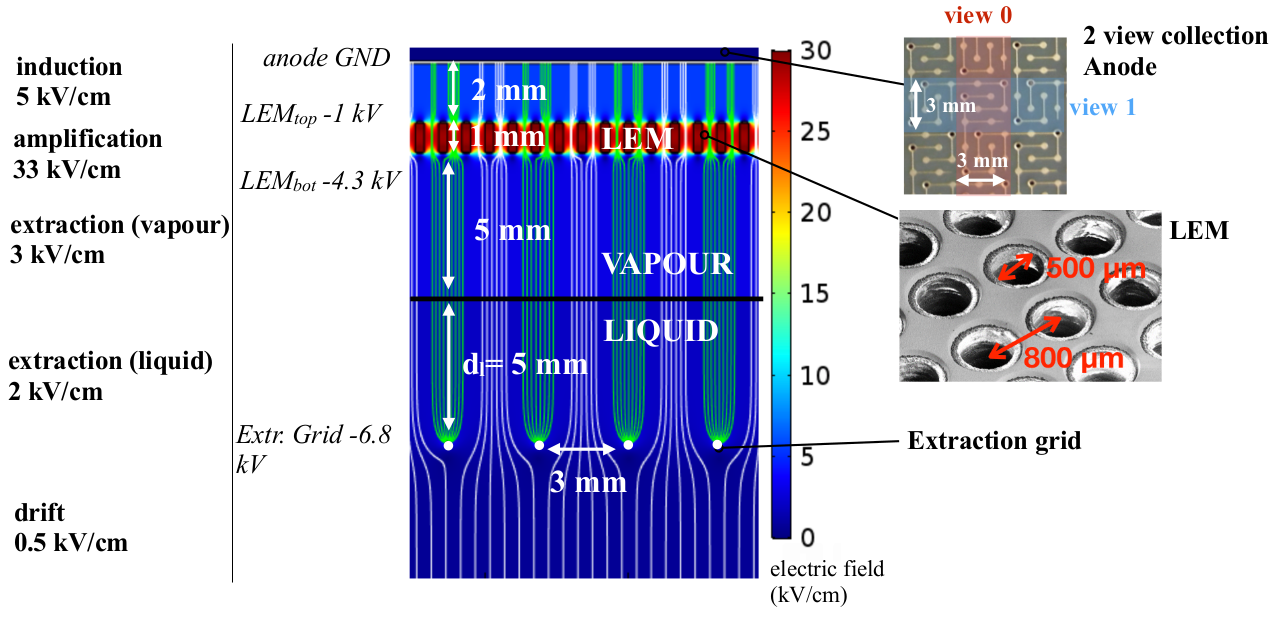
\includegraphics[width=\textwidth,keepaspectratio]{crp_fields.png}\end{center}
%                \caption[Champs électriques d'un  \gls{crp}.]{Illustration des trois principales zones d'un \gls{crp} de \gls{dlartpc}. Les champs et potentiels électriques indiqués correspondent à l'exploitation réussie d'une \gls{dlartpc} ayant atteint des gains effectifs de l'ordre de 20 \cite{Aimard2018,Cantini2014}.}
%                \label{fig::crp_fields}
%            \end{figure}
%            \begin{figure}[htbp]
%                \begin{subfigure}[b]{\textwidth}
%          \begin{center}\includegraphics[width=\textwidth,keepaspectratio]{crp_\TOO{}.png}\end{center}
%          \caption[\gls{crp} du prototype \TOO{}]{Schéma explosé du \gls{crp} du prototype \TOO{}. Les flèches rouges représentent les câbles de suspensions \cite{Aimard2018}.}
%          \label{fig::crp_\TOO{}}
%                \end{subfigure}
%                \begin{subfigure}[b]{\textwidth}
%          \begin{center}\includegraphics[width=\textwidth,keepaspectratio]{crp_\SSS{}_complete.png}\end{center}
%          \caption[\glspl{crp} du démonstrateur \SSS{}]{Schéma des \glspl{crp} du démonstrateur \SSS{}. L'un d'eux est représenté plus bas pour illustrer le fait qu'il y a 4 \glspl{crp}. Chacun mesure $3\times\SI{3}{\meter\squared}$. Les trais gris verticaux représentent les câbles de suspensions. La grille d'extraction n'est pas représentée sur ce schéma. \cite{CRPdesign}}
%          \label{fig::crp_\SSS{}}
%                \end{subfigure}
%                \caption{Schéma des \glspl{crp} de \protodp{}}
%            \end{figure}
%        
%            Le \gls{crp} a pour rôle:
%            \begin{enumerate}
%                \item L'extraction depuis l'argon liquide vers l'argon gazeux des électrons de dérives
%                \item L'amplification de ces électrons
%                \item La collecte du signal ainsi créé
%            \end{enumerate}
%            Toutes ces étapes sont réalisées grâce à trois champs électriques différents:
%            \begin{enumerate}
%                \item Le champ d'extraction, créé par une différence de potentielle entre la grille d'extraction et le bas du dispositif d'amplification. Sa mission est d'extraire un maximum d'électron du liquide vers le gaz en un temps aussi court que possible.
%                \item Le champ d'amplification, créé par une différence de potentielle à travers le dispositif d'amplification
%                \item Le champ d'induction, créé par un différence de potentiel entre le haut du dispositif d'amplification et les anodes de lecture
%            \end{enumerate}
%            La \autoref{fig::crp_fields} résume les points suivants : la grille d'extraction se situe $\SI{5}{\milli\meter}$ sous le niveau d'argon liquide, le bas du dispositif d'amplification se situe $\SI{5}{\milli\meter}$ au dessus du liquide. La tension appliquée entre les deux de $\SI{2.5}{\kilo\volt}$ correspondant à un champ électrique dans le liquide de $\SI{2}{\kilo\volt\per\centi\meter}$ ($\SI{3}{\kilo\volt\per\centi\meter}$ dans le gaz). Une étude \cite{guschin} a montré qu'à ces tensions, la totalité des électrons peut être extraite du liquide vers le gaz.
            
%            Le dispositif d'amplification est un ensemble de plusieurs \glspl{lem}, décrits en détails en \autoref{sec::LEM}, d'une épaisseur de $\SI{1}{\milli\meter}$ à travers laquelle est appliquée une tension de $\SI{3.5}{\kilo\volt}$, correspondant à un champ électrique d'environ $\SI{35}{\kilo\volt\per\centi\meter}$. De précédentes expériences \cite{Badertscher2011,Cantini2014} ont montré qu'un gain de l'ordre de 20 est atteignable à cette tension.
            
%            Les anodes, décrites en \autoref{sec::anode}, sont situées $\SI{2}{\milli\meter}$ au dessus des \glspl{lem}. Une tension de $\SI{1}{\kilo\volt}$ entre les anodes et le haut des \glspl{lem} créé un champ d'induction de $\SI{5}{\kilo\volt\per\centi\meter}$, qui doit alors correspondre à un probabilité de collection de charge optimale (voir \autoref{sec::efficacites}).
            
%            Les \glspl{lem} et anodes sont fixés sous des supports en fibre de verre G10, eux même fixés sous un squelette en acier inoxydable pour le prototype \TOO{} ou en Invar pour le démonstrateur \SSS{} (voir \autoref{sec::crp_structure}). La grille d'extraction est constituée de fils d'acier inoxydable, chacun tendu à $\SI{1.5}{\newton}$ à température ambiante sur des \glspl{pcb}, eux même fixés sur les bords des supports en G10. Le \gls{crp} est désolidarisé du reste du cryostat, il est donc possible de l'assembler et de le tester à part. Un système de câbles et poulies permet d'ajuster la position du \gls{crp} au dessus du liquide. La \autoref{fig::crp_\TOO{}} et la \autoref{fig::crp_\SSS{}} montrent respectivement le \gls{crp} du prototype \TOO{} et un \gls{crp} du démonstrateur \SSS{}. Le prototype \TOO{} n'a qu'un \gls{crp} recouvrant toute sa surface, mais le démonstrateur \SSS{} a quatre \gls{crp} de $3\times\SI{3}{\meter\squared}$, indépendants entre eux. Due à des retards de production, seuls deux de ces \gls{crp} sont instrumentés. Sur les deux autres, les \glspl{lem} et anodes ont été remplacés par des \glspl{pcb} mis à la masse.
%            
%            Le \gls{crp} est munie de plusieurs capteurs de pression, de température ainsi que de niveau d'argon liquide afin de suivre en direct les conditions à l'intérieur du détecteur et de pouvoir ajuster le niveau du \gls{crp} par rapport au liquide.
        
%    \subsection{Les contraintes techniques et la structure}\label{sec::crp_structure}
%            
%            Le \gls{crp} doit respecter plusieurs contraintes techniques \cite{CRPdesign} pour permettre une lecture efficace et fidèle de la charge:
%            
%            \begin{itemize}
%                \item Il doit être le plus plat possible, afin que l'interface liquide-gaz si situe bien au milieu de la distance grille--\gls{lem} pour tout le \gls{crp}. La tolérance fixée pour le démonstrateur \SSS{} est de \SI{0.5}{\milli\meter}, celle atteinte dans le prototype \TOO{} est de \SI{1}{\milli\meter} \cite{Aimard2018}.
%                \item Il doit supporter des variations de température importante sans se déformer de manière significative : le \gls{crp} est assemblé à température ambiante et descend ensuite à mois de \SI{90}{\kelvin}
%                \item Il doit être possible d'ajuster la position du \gls{crp} par rapport au niveau d'argon liquide à \SI{0.05}{\milli\meter} près.
%                \item Le démonstrateur \SSS{} est constitué de 4 \gls{crp}. La distance entre eux doit être de \SI{10}{\milli\meter} maximum
%                \item Comme le \gls{crp} est assemblé à part du reste du détecteur, il doit être transportable
%                \item Le \gls{crp} du démonstrateur \SSS{} doit être un élément utilisable dans la future expérience \gls{dune}, dont un module de détection sera constitué d'une trentaine de ces \gls{crp}
%            \end{itemize}
%            
%            Afin de satisfaire ces contraintes, la structure principale des \glspl{crp} du démonstrateur \SSS{} est faite en Invar, un alliage de fer et de nickel dont le coefficient de dilatation thermique est particulièrement faible (\SI{1.5e-6}{\per\kelvin} entre \SI{22}{\celsius} et \SI{-186}{\celsius}). La structure du \gls{crp} du prototype \TOO{} est elle faite en acier inoxydable.
%            
%            Les \glspl{lem} et anodes sont montés sur des cadres en G10 (neuf dans le \SSS{} et trois dans le \TOO{}), de la fibre de verre feuilletée solide et électriquement isolante. Des mesures de contraction thermique réalisées en 2015 ont donné pour le G10 utilisé dans \protodp{} des coefficients de l'ordre de \SI{e-5}{\per\kelvin}, proches du ceux des \glspl{las}. Le G10 et les \glspl{las} réagissent donc de la même manière aux différents changements de température. Sur les trois mètres du \gls{crp} du démonstrateur \SSS{}, la contraction maximum mesurée est d'environ \SI{6}{\milli\meter}. L'Invar se contractant beaucoup moins, les cadres en G10 sont fixés sur la structure en Invar avec des éléments permettant au G10 de se contracter librement.
%            
%            Le positionnement vertical et horizontal des \glspl{crp} se fait grâce à un système de suspension. Un \gls{crp} (dans le \SSS{} comme dans le \TOO{}) est suspendu par trois câbles motorisés, passant par des conduites isolantes traversant le couvercle du détecteur pour atteindre le \gls{crp}. Ils permettent une amplitude verticale de \SI{98}{\milli\meter} dans le démonstrateur \SSS{} (\SI{40}{\milli\meter} dans le prototype \TOO{}) avec une précision de \SI{100}{\micro\meter} et une amplitude horizontale de \SI{26}{\milli\meter} dans le démonstrateur \SSS{}. Le \TOO{} n'est pas pourvu d'un système de positionnement horizontal.
%            
%            Les \glspl{las} sont assemblés et fixés sur le cadre en G10 par des entretoises en PEEK (polyétheréthercétone) assurant l'espacement de \SI{2}{\milli\meter} entre les \glspl{lem} et les anodes. Les extrémités de ces entretoises sont filetées, un côté est vissé directement dans le G10.
            
%    \subsection{Électronique : signaux, alimentation}
%            
%            Les signaux sont apportés vers l'extérieur par des conduites similaires à celles des câbles de suspension, remplies d'azote \cite{Acciarri2016a} traversant le couvercle du détecteur. Elles sont faites de manière à ce que l'électronique Frontend soit accessible pour d'éventuelles réparations sans contaminer l'argon. Les cartes Frontend (des circuits CMOS ASIC) sont située en bas des conduites et refroidie à \SI{110}{\kelvin}. L'électronique numérique et le \gls{daq} sont situés en dehors du cryostat.
%            
%            L'alimentation haute tension passe elle aussi par des conduites isolante, et est distribuée aux \gls{lem}, aux anodes et à la grille d'extraction par des câbles coaxiaux courant le long de la structure du \gls{crp}. Dans le prototype \TOO{}, chaque face de chaque \gls{lem} ainsi que chaque anode a sa propre alimentation. Dans le démonstrateur \SSS{}, les faces hautes des \glspl{lem} sont alimentées par groupe de neuf.
%            
%            Les anodes sont reliées entre elles via des nappes et des connecteurs KEL formant des canaux de trois mètres de long dans le \SSS{} et trois ou un mètre dans le \TOO{}.
%            
    \subsection{Les anodes}\label{sec::anode}
        
%            \begin{figure}[htbp]
%                \begin{center}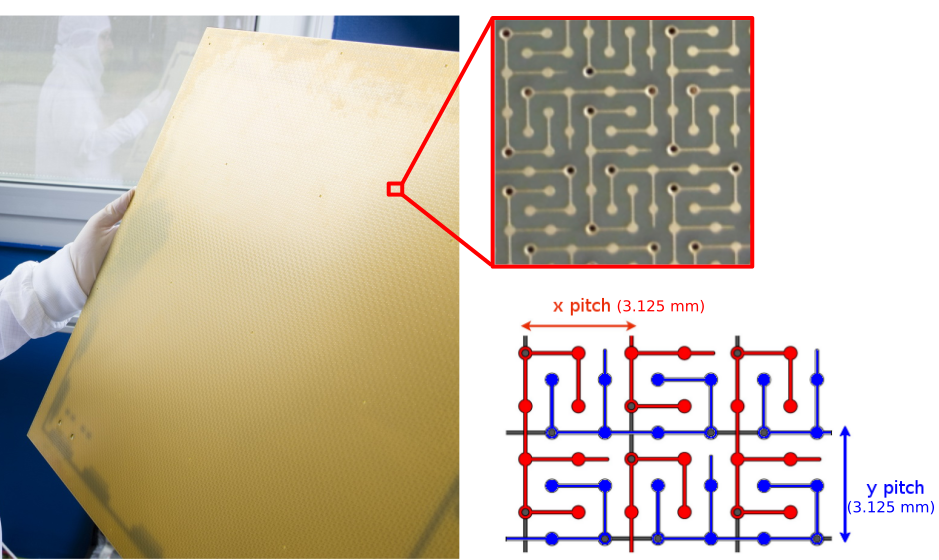
\includegraphics[width=\textwidth,keepaspectratio]{anode.png}\end{center}
%                \caption[Agrandissement d'une anode de lecture.]{Agrandissement d'une anode de lecture. L'orthogonalité des canaux de lecture des vues $x$ et $y$ facilite la reconstruction des événements, la dispositions en plusieurs couches assure une capacitance de $\SI{160}{\pico\farad\per\meter}$ \cite{Cantini2013}.}
%                \label{fig::anode}
%            \end{figure}
%            \begin{figure}[htbp]
%                \begin{center}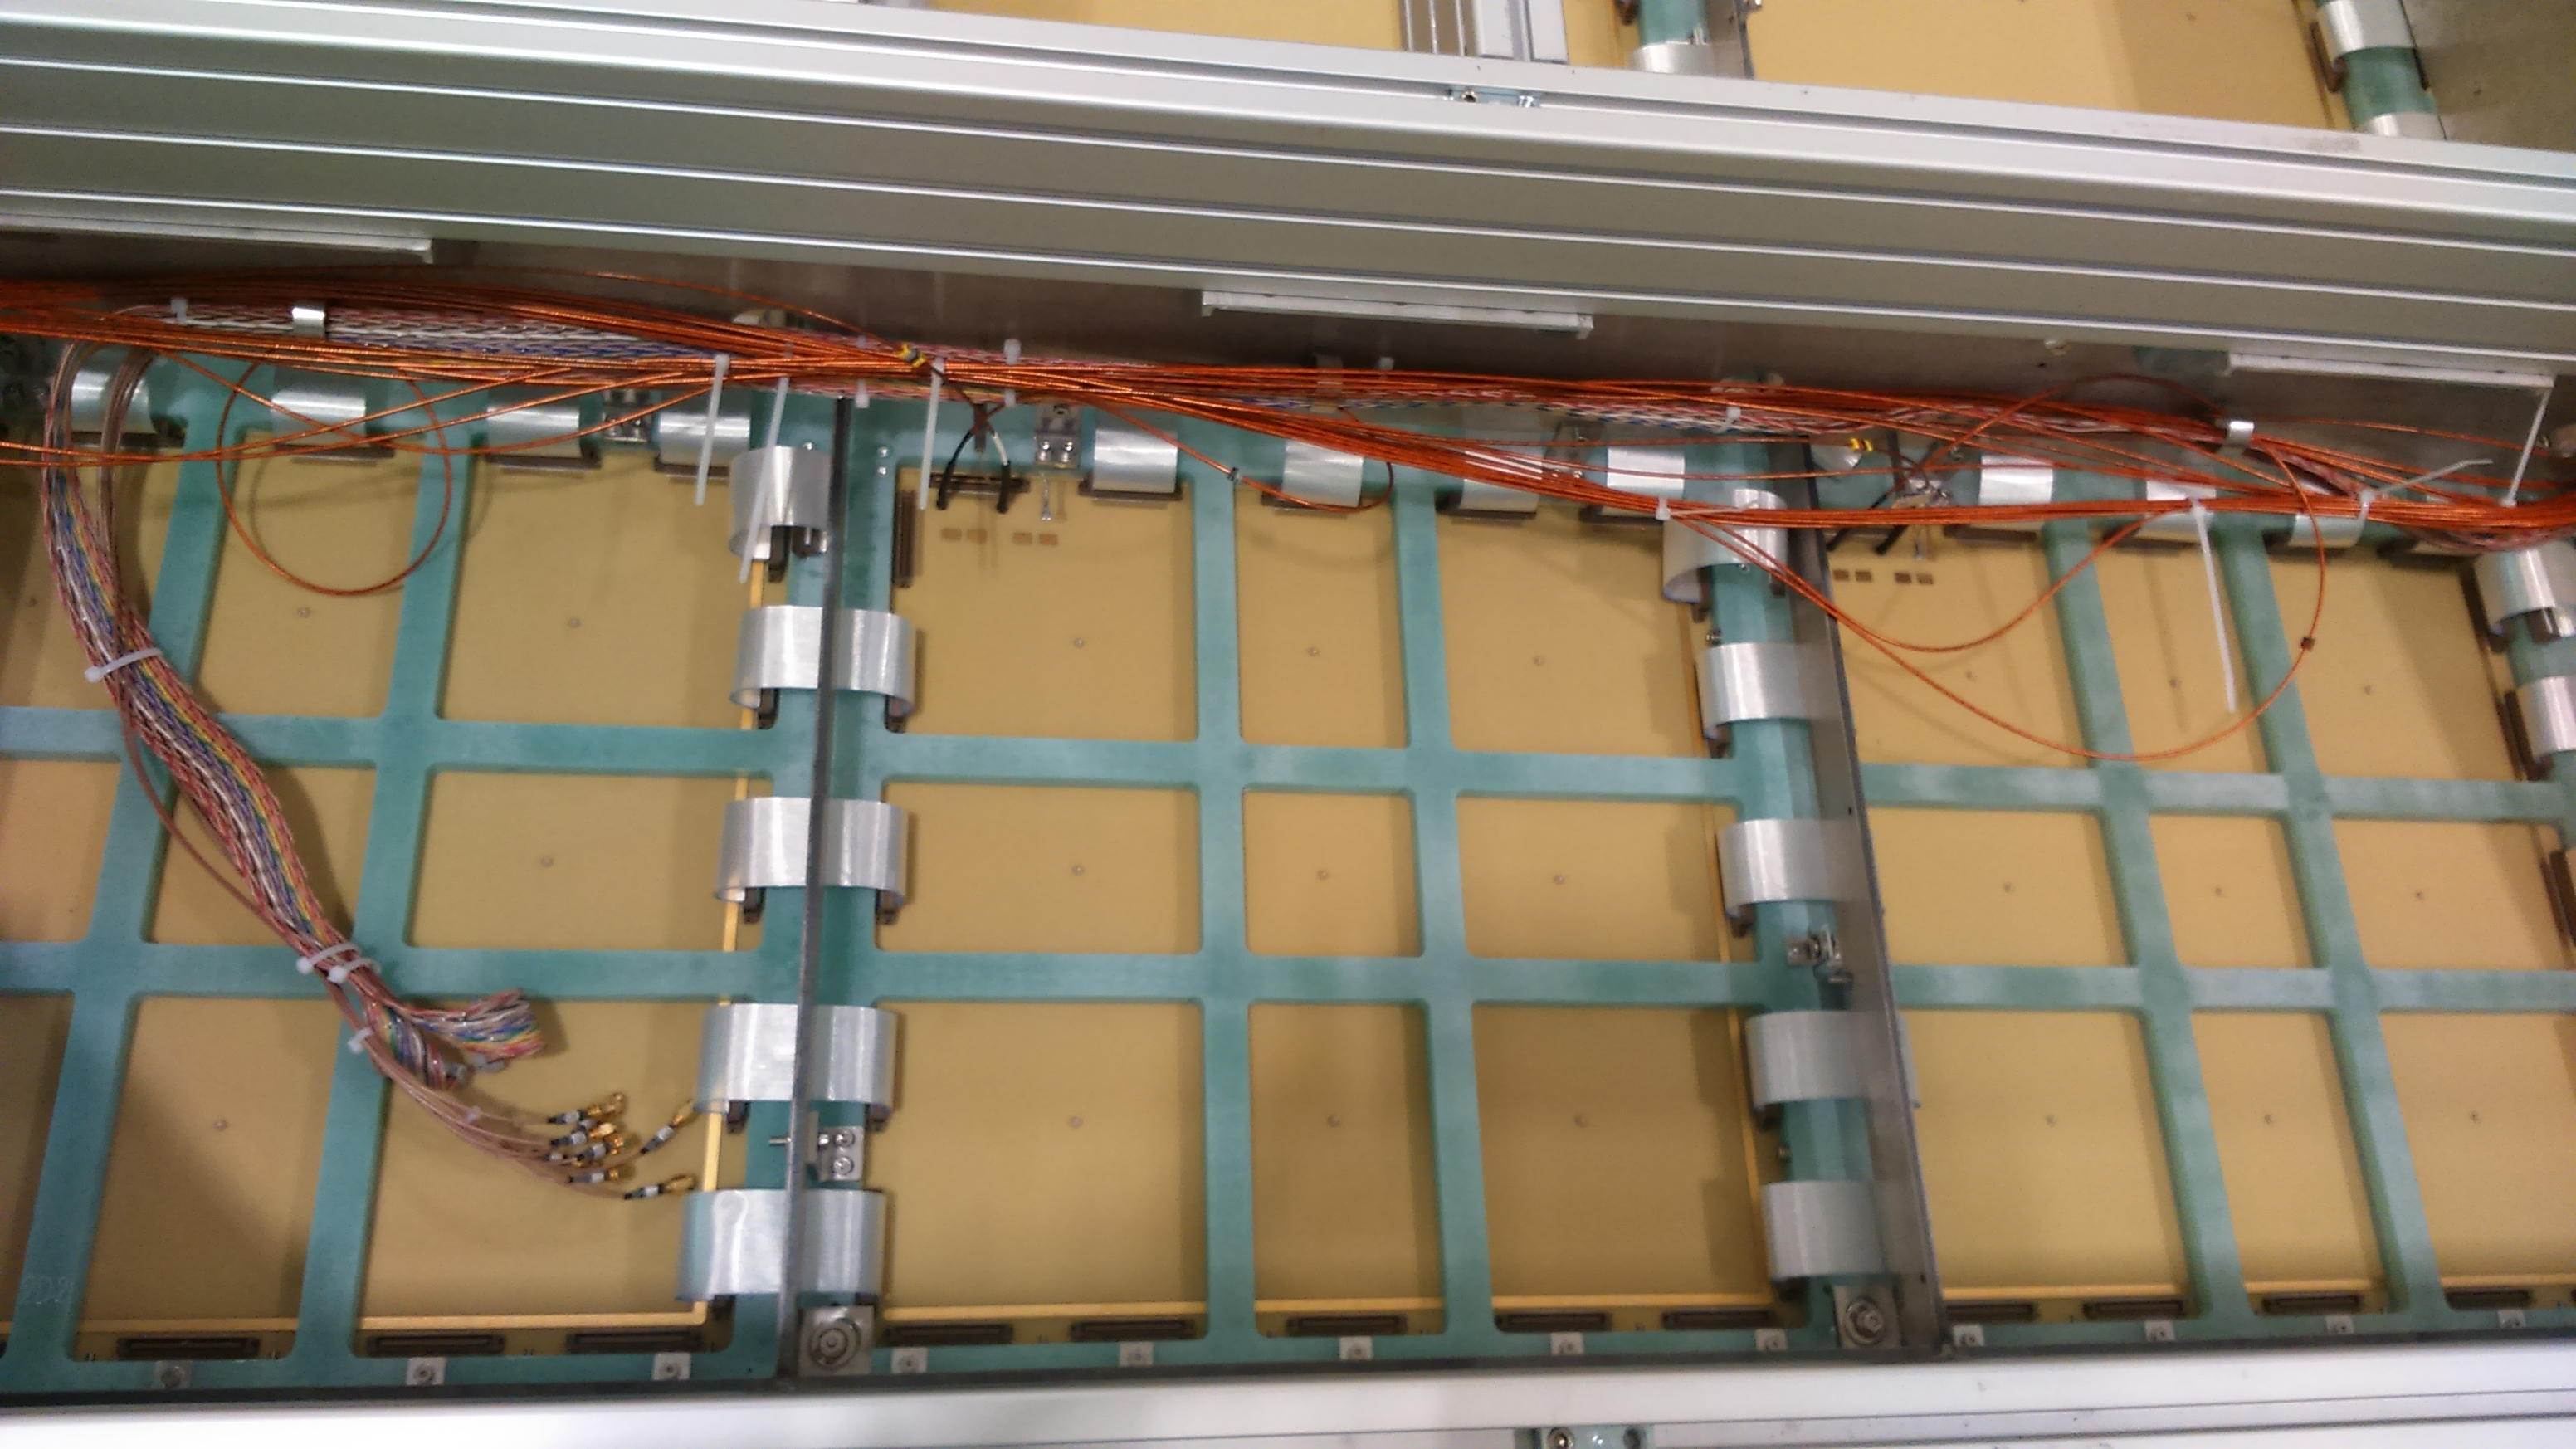
\includegraphics[width=\textwidth,keepaspectratio]{connecteurs2.JPG}\end{center}
%                \caption[Vue du dessus d'un \gls{crp} du démonstrateur \SSS{}.]{Vue du dessus d'un \gls{crp} du démonstrateur \SSS{}. On peut y voir les câbles d'alimentation haute tension des \glspl{lem} le long de la structure en Invar ainsi que les nappes reliant les connecteurs KEL entre les anodes, formant des canaux de \SI{3}{\meter}.}
%                \label{fig::connecteurs}
%            \end{figure}
            
      Le modèle des anodes (voir \autoref{fig::anode}), fabriquées par la compagnie ELTOS\footnote{\url{http://www.eltos.com/en/}} en Italie, est le résultat de tests réalisés au CERN par l'\gls{ethz} dans le prototype de \gls{dlartpc} de \threeL{}\cite{Cantini2013} en vue de réduire au maximum la capacitance, et donc le bruit, tout en ayant un partage égale de charge entre deux vues perpendiculaires, facilitant la reconstruction des événements et leur analyse.
            
      Chaque anode est un \gls{pcb} de quatre couches, avec une surface de  $50\times\SI{50}{\centi\meter\squared}$ et comporte deux jeux de canaux perpendiculaires, \numprint{160} pour la vue $x$ et \numprint{160} pour la vue $y$. La largeur d'un canal est de $\SI{3.125}{\milli\meter}$ et correspond à deux lignes inter-connectées, de cuivre recouvertes d'or. Les canaux sont ramenés par groupes de 32 vers l'autre surface de l'anode jusqu'à des connecteurs KEL de 68 pins, dont les 36 pins restant sont mis à la masse. Dans le prototype de \TOO{} comme dans le démonstrateur de \SSS{}, ces connecteurs sont reliés entre eux d'une anode à l'autre afin de former des canaux continus de $\SI{1}{\meter}$, $\SI{3}{\meter}$ ou $\SI{6}{\meter}$. La capacitance linéique est alors de $\SI{160}{\pico\farad\per\meter}$, correspondant à un bruit de fond inférieur à \numprint{2000} électrons\cite{Aimard2018} pour les longs canaux de $\SI{3}{\meter}$ du prototype de \TOO{}.
            
      Les anodes ont été inspectées visuellement par le fabricant avant envoi, et la continuité de leurs canaux a été testée par Saclay (plus de détails en \autoref{sec::test_anode}).
        
    \subsection{Les Larges Multiplicateurs d'Électrons (LEM)}\label{sec::LEM}

      \begin{figure}[htbp]
        \begin{subfigure}[t]{0.48\textwidth}
          \centering
          \captionsetup{width=.95\linewidth}
          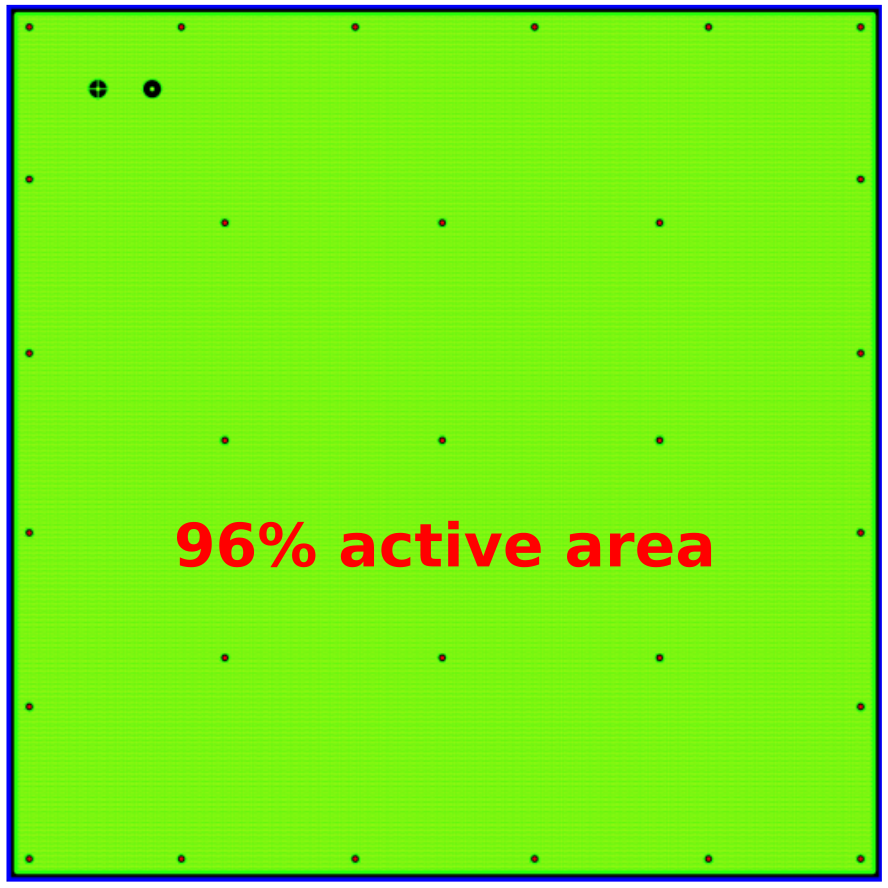
\includegraphics[width=0.8\textwidth,keepaspectratio]{CFR-34.png}
          \caption{\label{fig::cfr34}Modèle de LEM CFR-34 utilisé dans le prototype de \TOO{}. Les zones dépourvues de trous d'amplifications aux bords et autour des trous des vis et des connecteurs haute tension sont plus petites que celles du modèle CFR-35, la surface active totale étant de 96\,\%.}
        \end{subfigure}
        \hfill
        \begin{subfigure}[t]{0.48\textwidth}
          \centering
          \captionsetup{width=.95\linewidth}
          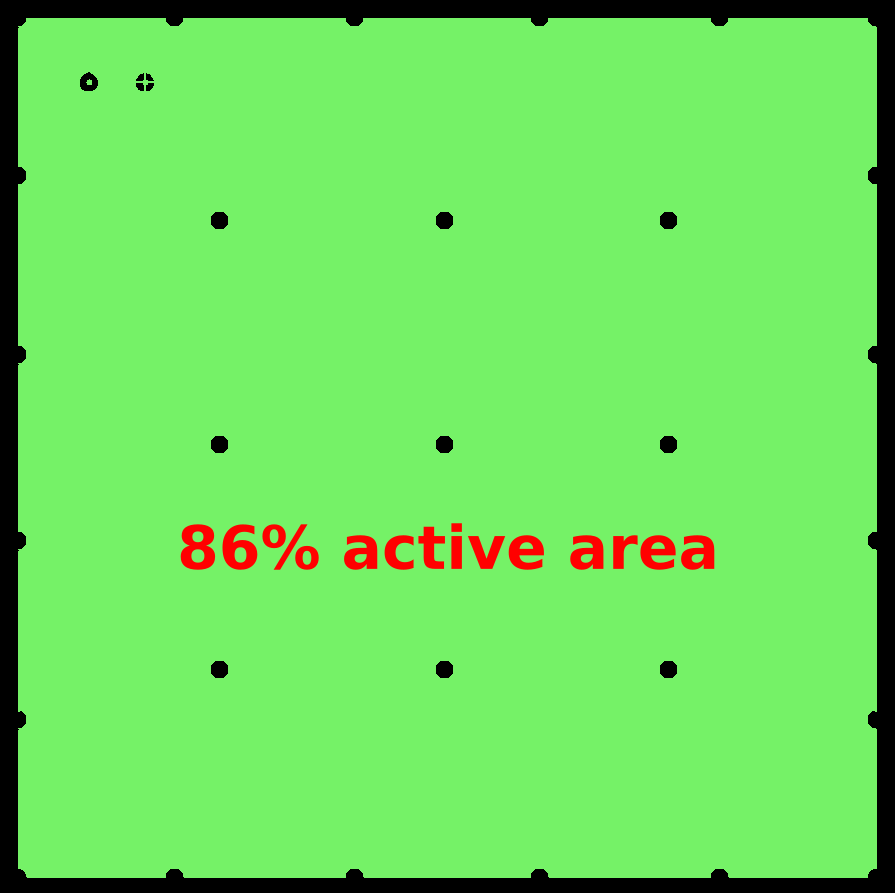
\includegraphics[width=0.8\textwidth,keepaspectratio]{CFR-35.png}
          \caption{\label{fig::cfr35}Modèle de \gls{lem} CFR-35 utilisé dans le démonstrateur de \SSS{}. Les zones dépourvues de trous d'amplifications ont été agrandies par rapport au modèle CFR-34 qui montrait des difficultés à tenir des tensions de l'ordre de \SI{3}{\kilo\volt}, ce qui ne permet pas d'atteindre un gain de 20. Ce nouveau modèle est stable à \SI{3.1}{\kilo\volt}, mais sa surface active totale est réduite à 86\,\%.}
        \end{subfigure}
        \caption[Modèle de LEM CFR-34 et CFR-35]{Fichier Gerber des modèles de \gls{lem} CFR-34 et CFR-35.}
        \label{fig::cfrs}
      \end{figure}

%      Les \glspl{lem} sont l'élément central d'une \gls{dlartpc}. Ce sont eux qui vont permettre l'amplification du signal dans la phase gazeuse. Produits de plusieurs dizaines d'années de recherche et développement, ils ont prouvé être mieux adaptés aux amplifications dans les gaz nobles que les techniques utilisant des chambres à fils, des GEM ou des micro-mégas (\cite{Buzulutskov2000,Breskin2008}). Ce sont des \glspl{pcb} constitués d'une plaque de résine époxy PANASONIC R-1566W (\gls{fr4}) recouverte de chaque côté par une fine couche de cuivre. Des trous sont percés à travers cette plaque, au travers desquelles les électrons primaires, issues de l'interaction d'une particule avec l'argon liquide plus bas, sont accélérés par une forte différence de potentielle appliquée entre les deux couches de cuivre, créant un champ électrique de l'ordre de $\SI{30}{\kilo\volt\per\centi\meter}$. Ceci permet alors de déclencher une avalanche de Townsend (voir \autoref{sec::townsend_avalanche}) et donc d'amplifier le signal.
            
%            Un effet à prendre en compte dans les détecteurs utilisant des amplificateurs comme les \glspl{lem} est le chargement de ces derniers. En effet, les lignes de champs à travers les \glspl{lem} sont tels que des électrons vont pouvoir terminer leur course sur le \gls{fr4} au lieu de traverser le dispositif. Une accumulation de ces électrons diminuera alors le champ d'amplification, entraînant une baisse de gain. Ce phénomène, étudié dans cet article \cite{Cantini2014}, peut être décrit par une décroissance exponentielle du gain à laquelle est associée un temps caractéristique (que l'on appellera temps de charge) qu'il convient de mesurer. Comme une exploitation des résultats n'a vraiment de sens qu'à gain constant, il est préférable de diminuer ce temps de charge afin d'atteindre au plus vite un régime permanent.
            
%            Un autre problème potentielle est que des tensions trop importantes peuvent entraîner des décharges soudaines, entre la grille de un ou plusieurs \gls{lem}, au travers d'un ou plusieurs \gls{lem} ou entre un ou plusieurs \gls{lem} et les anodes. Ces décharges ont, par exemple, grandement limité la prise de données avec le prototype \TOO{} qui n'a pas réussi à atteindre les tensions souhaitées en \autoref{sec::crp_intro}.
            
%      Les \glspl{lem} de \protodp{} ont une surface de $50\times\SI{50}{\centi\meter\squared}$ permettant de couvrir les $\SI{36}{\meter\squared}$ du démonstrateur \SSS{} avec 144 \glspl{lem}, et une épaisseur de $\SI{1}{\milli\meter}$. Ils sont percés de \numprint{400000} trous de $\SI{500}{\micro\meter}$ de diamètre, répartis selon un motif hexagonale sur la surface du \gls{lem} (voir \autoref{fig::lem}). Chaque trou est entouré d'un anneau dépourvu de cuivre d'une épaisseur de $\SI{40}{\micro\meter}$ appelé rim, servant à assurer la stabilité en tension du \gls{lem}\cite{Breskin2008}. L'épaisseur de cuivre est de $\SI{60}{\micro\meter}$. Les \glspl{lem} sont percés de \numprint{29} trous de fixation au travers desquelles passent les entretoise et deux trous pour passer les connecteurs haute tension. Les spécifications précises sont décrites dans le \autoref{tab::lem_commun}.
            
      Les \glspl{lem} utilisés dans le prototype de \TOO{} ont un bord dépourvu de cuivre de $\SI{2}{\milli\meter}$, suivi d'un bord de $\SI{2}{\milli\meter}$ de cuivre dépourvu de trous d'amplification. Des zones similaires sont présentes également autour des trous de fixation et des connecteurs haute tension. Les effets de ces zones sur la collection de charge et la résolution en énergie est présentée en \autoref{sec::dead_zones}. Des tests de tenue en haute tension effectués à Saclay (voir \autoref{sec::test_HT}) sur les \glspl{lem} destinés au démonstrateur de \SSS{} ont permis de montrer que ce modèle (appelé CFR-34) ne permettait pas d'atteindre la tension de \SI{3.1}{\kilo\volt} qui correspond à un gain effectif attendu de 20 (\autoref{fig::3L_gain}). Un nouveau modèle (appelé CFR-35) a alors été proposé, avec des bords plus larges. Ces derniers sont constitués d'une zone de $\SI{1}{cm}$ dépourvue de cuivre suivi d'une zone de $\SI{5}{mm}$ de cuivre sans trous d'amplification  (voir \autoref{fig::cfrs}). C'est ce modèle qui a été choisi pour le démonstrateur \SSS{}. Les spécifications précises des deux modèles sont décrites dans le \autoref{tab::lem_diff}.
            
      \begin{table}
        \centering
        \begin{tabular}{|l|c|c|}
          \hline
           & valeur & tolérance \\
          \hline
          Épaisseur d'époxy & \SI{1}{\milli\meter} & \\
          Épaisseur de cuivre & \SI{60}{\micro\meter} & \\
          Couche de finition & \SI{5}{\micro\meter} Ni$+\SI{0.1}{\micro\meter}$ Au & \\
          Épaisseur totale & \SI{1.065}{\milli\meter} &  $-60/+\SI{20}{\micro\meter}$ \\
          \begin{tabular}{@{}l@{}}Uniformité de \\ l'épaisseur\end{tabular} & $\pm \SI{40}{\micro\meter}$ & \\
          Largeur du RIM & \SI{40}{\micro\meter} & $\pm\SI{4}{\micro\meter}$ \\
          Surface totale &  $499.5\times\SI{499.5}{\milli\meter\squared}$ & $+0/-\SI{0.2}{\milli\meter}$ \\
          Nombre de trous & $\sim400000$ & \\
          Diamètre des trous & $\SI{0.5}{\milli\meter}$ & $-0/+\SI{10}{\micro\meter}$ \\
          \begin{tabular}{@{}l@{}}Distance centre à \\ centre entre \\ deux trous\end{tabular}  & $\SI{0.8}{\milli\meter}$ & \\
          \hline
        \end{tabular}
        \caption[Caractéristiques des LEMs communes aux deux modèles utilisés dans WA105]{\label{tab::lem_commun}Caractéristiques des \glspl{lem} communes aux deux modèles utilisés dans \gls{wa105}.}
      \end{table}
            
      \begin{table}
        \centering
        \begin{tabular}{|l|c|c|}
          \hline
           & CFR-34 & CFR-35\\
          \hline
          Bord -- zone sans cuivre & \SI{2}{\milli\meter} & \SI{10}{\milli\meter}\\
          Bord -- zone avec cuivre sans trous & \SI{2}{\milli\meter} & \SI{5}{\milli\meter}\\
          Trous de vis -- diamètre sans cuivre & \SI{4.2}{\milli\meter} & \SI{10}{\milli\meter} \\
          Trous de vis -- anneau sans trous &  \SI{1.1}{\milli\meter} & \SI{5}{\milli\meter} \\
          Trous de connecteur -- diamètre sans cuivre & \SI{10}{\milli\meter} & \SI{10}{\milli\meter} \\
          Trous de connecteur -- anneau sans trous & \SI{1}{\milli\meter} & \SI{5}{\milli\meter} \\
          \hline
        \end{tabular}
        \caption[Caractéristiques spécifiques aux modèles de LEM utilisés dans \protodp{}]{\label{tab::lem_diff}Caractéristiques spécifiques aux modèles de \gls{lem} utilisés dans \protodp{}.}
      \end{table}

  \section{Préparation, caractérisation et test à l'IRFU et au CERN}
    
    Le \gls{cea} Saclay était en charge de la production et les tests des des \glspl{lem} des deux \glspl{crp} instrumentés démonstrateur de \SSS{}, ainsi que les tests des anodes de ces même \glspl{crp}. Un appel d'offre pour les modèles a été lancé en février 2017 et l'entreprise ELTOS a été retenue. Il a été demandé à l'entreprise d'effectuer plusieurs mesures sur les \glspl{lem} produits : l'épaisseur de la plaque d'époxy et des couches de cuivre, l'épaisseur des RIMs, la taille des trous d'amplification ainsi que les caractéristiques diélectriques. Le \gls{cea} a par la suite effectué des mesures complémentaires de l'épaisseur totale, ce paramètre ayant un impact particulièrement important sur le gain (voir \autoref{sec::townsend}). Des tests de tenus en haute tension ainsi que des mesures de gain avec une source radioactive dans de l'argon gazeux à densité équivalente à celle de la phase gazeuse d'une \gls{dlartpc} ont été réalisés dans une enceinte haute pression construite dans ce but. Enfin, des tests de continuité des canaux de lecture des anodes ont également été réalisés.
        
    \subsection{Production et préparation des LEM}
        
      La réalisation d'un \gls{lem} par ELTOS commence par un perçage des plaques d'époxy préalablement couvertes de cuivre, avec changement fréquent des forets. S'en suit un nettoyage des résidus d'époxy et de métal dans les trous, puis un polissage pour arrondir les bords des trous. Les RIMs sont obtenus par micro-etching. Un traitement de surface nickel/or est appliqué. Le \gls{lem} est détouré à ses dimensions finales  et les zones mortes sur les bords sont réalisées par gravure chimique. Enfin, le \gls{lem} est nettoyé, rincé et étuvé.
          
      Sont ensuite effectuées les mesures décrites en \autoref{sec::thickness_comparison_eltos} pour s'assurer de la conformité au cahier des charges.
      
      Entre juillet 2017 et septembre 2018, le \gls{cea} a reçu et testé les 72 \glspl{lem} du démonstrateur \SSS{}. Une fois les \glspl{lem} arrivés à l'\gls{irfu}, ils sont inspectés visuellement et les imperfections sont relevées. Ils sont ensuite envoyés à la métrologie afin que leurs épaisseurs soient mesurées (voir \autoref{sec::epaisseur}).
      
      L'étape suivante est alors la soudure de connecteurs haute tension et le collage des entretoises en MACOR, qui permettront d'assurer une distance entre le \gls{lem} et l'anode de \SI{2}{\milli\meter}.
      
      \SI{24}{\hour} après le collage, les \glspl{lem} sont nettoyés pendant \numprint{3} minutes dans un bain à ultrasons d'eau désionisée et de lessive, à \SI{65}{\celsius} puis rincés d'abord à l'eau claire puis au Karcher avec de l'eau désionisée. Ils sont ensuite séchés une première fois avec un jet l'azote avant d'être séchés une seconde fois au four à \SI{80}{\celsius} pendant \numprint{3} heures. Ils sont ensuite polymérisés au four à \SI{160}{\celsius} pendant \numprint{3} heures.

      Ils sont ensuite placés dans une enceinte haute pression. Cette enceinte est dans un premier temps remplie d'air sec, ou une tension de \SI{4500}{\volt} est appliquée à travers le \gls{lem} afin de détruire les micro-poussières restantes. L'air sec est ensuite remplacé par de l'argon gazeux à \SI{3.3}{\bar}, recréant ainsi la densité de la phase gazeuse d'une \gls{dlartpc}. Sont alors effectués des tests de tenus en tension et des mesures de gain (voir \autoref{sec::test_HT}).
        
    \subsection{Les mesures d’épaisseur des LEM}\label{sec::epaisseur}
        
      \subsubsection{Motivation : impact sur le gain}
            
        \begin{figure}[htbp]
          \centering
          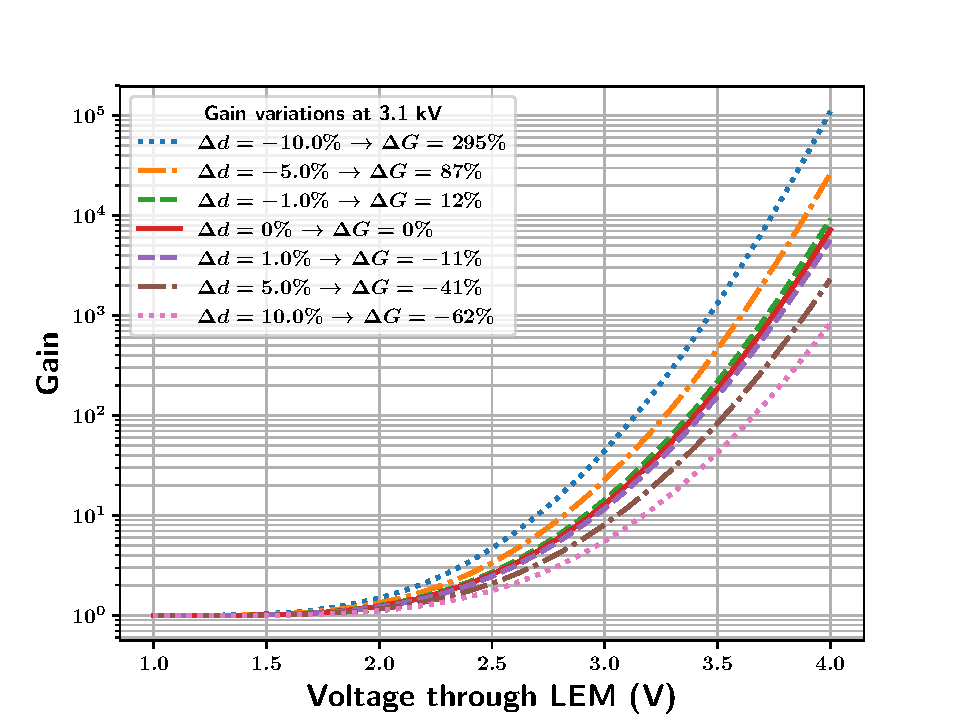
\includegraphics[width=0.8\textwidth,keepaspectratio]{influence_dx_gain.pdf}
          \caption[Influence de l'épaisseur d'un LEM sur le gain]{Influence attendue de l'épaisseur d'un \gls{lem} sur le gain, d'après le formule \eqref{eq::townsend_avalanche_2} ajustée aux données présentées dans \cite{Cantini2014}. On constate qu'à \SI{3.1}{\kilo\volt}, une variation de l'épaisseur de 1\,\% entraîne une variation du gain de l'ordre de 10\,\%.}
          \label{fig::thickness_influence_on_gain}
        \end{figure}
            
        La formule du gain à travers un dispositif amplificateur est rappelée ici (voir \autoref{sec::townsend} pour plus de détails) :
        \begin{equation}\label{eq::townsend_avalanche_2}
          G = e^{A\rho d e^{-B\rho /E}}
        \end{equation}
        Avec $\rho$ la densité de l'argon gazeux, $E$ le champ d'amplification dans le \gls{lem}, $A$ et $B$ des constantes dépendant du gaz et $d$ la longueur de la zone d'amplification. Cette longueur $d$ correspond dans le cas d'un \gls{lem} à son épaisseur. Ce paramètre apparaît deux fois, dans la première et dans la seconde exponentielle à travers le champ $E = V/d$, ses variations ont donc un impact significatif sur le gain (voir \autoref{fig::thickness_influence_on_gain}). Il est nécessaire de pouvoir quantifier ses variations pour les \glspl{lem} utilisés, nous avons donc mis en place un dispositif permettant de mesurer l'épaisseur des \glspl{lem} produits pour les deux \gls{crp} du \SSS{}. Les résultats ainsi obtenus sont comparés aux mesures obtenues par le fabricant, ELTOS, dans le \autoref{tab::mesures_eltos}.
                
        \subsubsection{Méthode expérimentale}
                %documentation dans hardware/lem_plaques/marbre_472
          La technique d'\acrfull{cci} (voir \autoref{fig::CCI}), est employée pour mesurer l'épaisseur des \glspl{lem}. L'image $S'$ d'une source polychromatique ponctuelle $S$ est créée à la surface de l'objet à mesurer grâce à une lentille convergente. Les rayons réfléchis en $S'$ retraversent la lentille et sont déviés grâce à un miroir vers un trou d'épingle $S''$, placé devant un spectromètre. La distance focale de la lentille dépend de la longueur d'onde, aussi seul un spectre très restreint de la lumière initiale atteindra le trou d'épingle. En faisant correspondre la longueur d'onde détectée à une distance à la lentille, il est ainsi possible de mesurer la distance entre la lentille et l'objet. Le crayon optique servant de source est monté sur un rail grâce à un chariot à coussin d'air, lui permettant de se déplacer sans frottement sur un axe $x$, dont la coordonnée est enregistrée au micron près. Le logiciel de mesure utilisé permet de visualiser en direct les variations de hauteurs au cours de la mesure. La forme des trous micrométriques des \glspl{lem} est visible sur la \autoref{fig::soft_measure_LEM}, issue de ce logiciel. %A noter que due à l'absence de motorisation du chariot sur coussin d'air, ce dernier était poussé à la main, ce qui ne garantissait pas une vitesse constante.
          
          \begin{figure}[htpb]
            \begin{subfigure}{0.48\textwidth}
              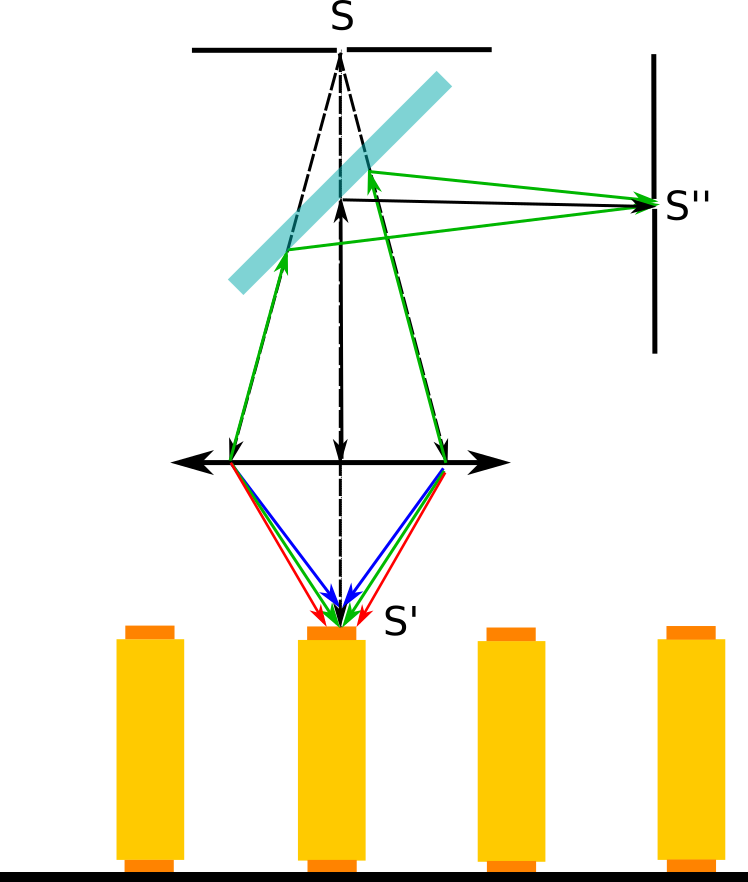
\includegraphics[width=0.8\textwidth,keepaspectratio]{CCI.png}
              \caption{\label{fig::CCI}Schéma de la méthode de mesure \gls{cci} servant à mesurer l'épaisseur des \glspl{lem}. Les blocs oranges et jaunes représentent une vue en coupe, à l'échelle, d'un \gls{lem} posé sur le marbre avec ses trous d'amplification.}
            \end{subfigure}
            \hfill
            \begin{subfigure}{0.48\textwidth}
              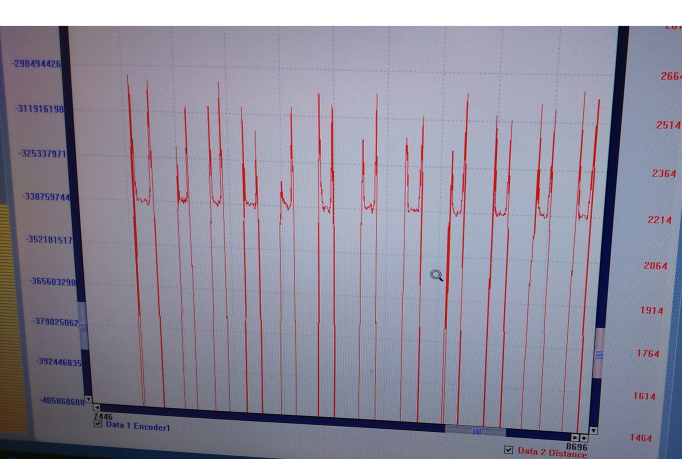
\includegraphics[width=\textwidth,keepaspectratio]{soft_measure_LEM.png}
              \caption{\label{fig::soft_measure_LEM}Représentation brute des données de mesure d'un \gls{lem} avec la technique \gls{cci}. Les grands pics sont coupés à l'analyse.}
            \end{subfigure}
            \caption[Schéma de principe et exemple de mesure de la surface d'un LEM avec la technique CCI]{Schéma de principe et exemple de mesure de la surface d'un \gls{lem} avec la technique \gls{cci}.}
          \end{figure}
          
           Le dispositif mesure la distance entre la surface et le crayon optique. Il faut donc disposer d'une surface plate uniforme sur laquelle poser l'objet à mesurer, qui servira de zéro, et aplatir l'objet. Dans notre cas, le zéro est donné  par un marbre micrométrique. Un exemple de mesure de variations de hauteur de ce marbre est présentée en \autoref{fig::marbre}. On constate que le marbre présente une légère pente, qui peut facilement être prise en compte dans les mesures du \gls{lem}. Le \gls{lem} est aplati par une plaque en acier inox percée de 25 trous à travers lesquels les mesures étaient effectuées, ainsi que des briques de plomb placées le long du chemin de mesure (voir \autoref{fig::plate_and_bricks}). Malgré cela, le trou de mesure situé le plus au centre du \gls{lem} présentait encore des variations de $10$ à $\SI{15}{\micro\meter}$ quand une pression supplémentaire était appliquée sur la plaque d'acier. Il a donc était décidé d'ignorer ce trou de mesure.

          \begin{figure}[htpb]
            \begin{subfigure}[t]{0.5\textwidth}
              \centering
              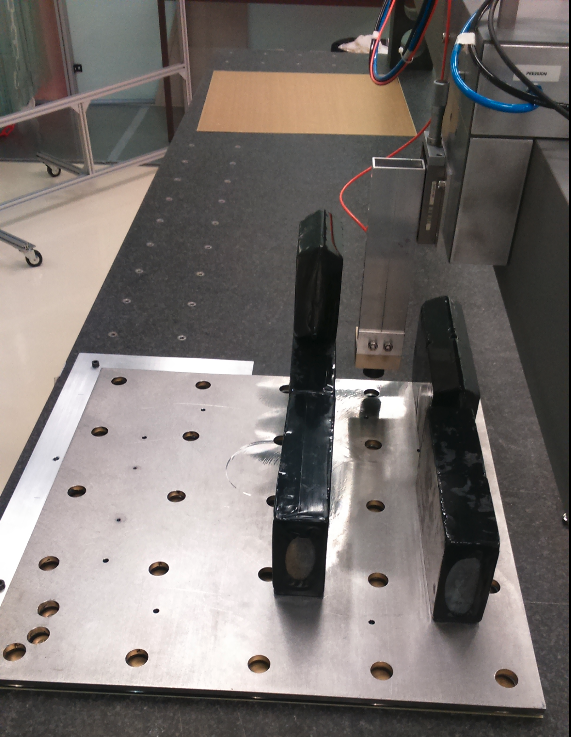
\includegraphics[width=\textwidth,keepaspectratio]{plate_and_bricks.png}
              \caption{\label{fig::plate_and_bricks}Système servant à aplanir le \gls{lem} sur le marbre. Le \gls{lem} est sous une plaque d'acier sur laquelle sont posées des briques de plomb le l'axe de mesure.}
            \end{subfigure}
            \hfill
            \begin{subfigure}[t]{0.395\textwidth}
              \centering
              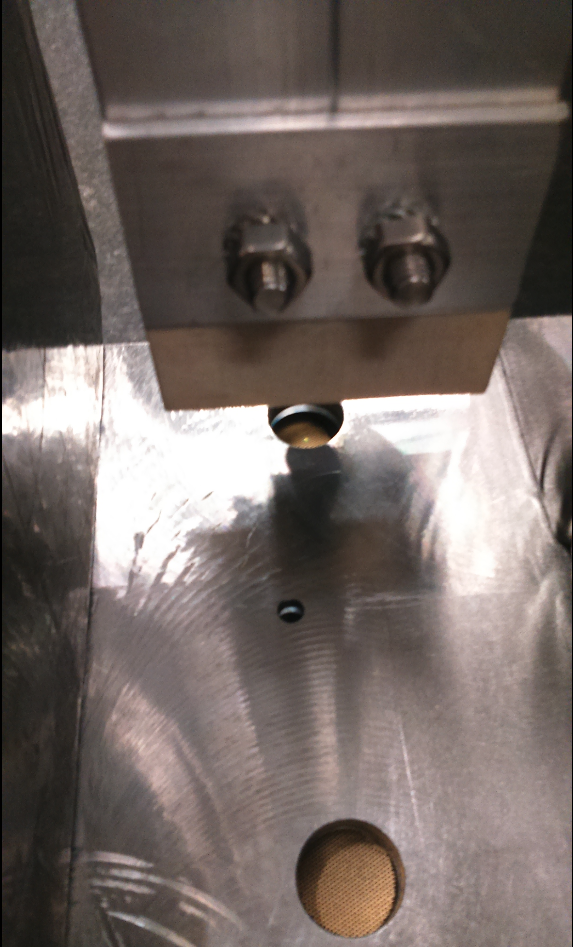
\includegraphics[width=\textwidth,keepaspectratio]{LEM_through_plate.png}
              \caption{\label{fig::LEM_through_plate}Vue du \gls{lem} mesuré à travers un trou de la plaque en acier. Le point vert correspond à la lumière du crayon optique.}
            \end{subfigure}
            \caption[Photographies du dispositif expérimental utilisé pour les mesures d'épaisseur des LEM]{\label{fig::dispositif_experimental}Photographies du dispositif expérimental utilisé pour les mesures d'épaisseur des \glspl{lem}.}
          \end{figure}

          \begin{figure}[htpb]
            \centering
            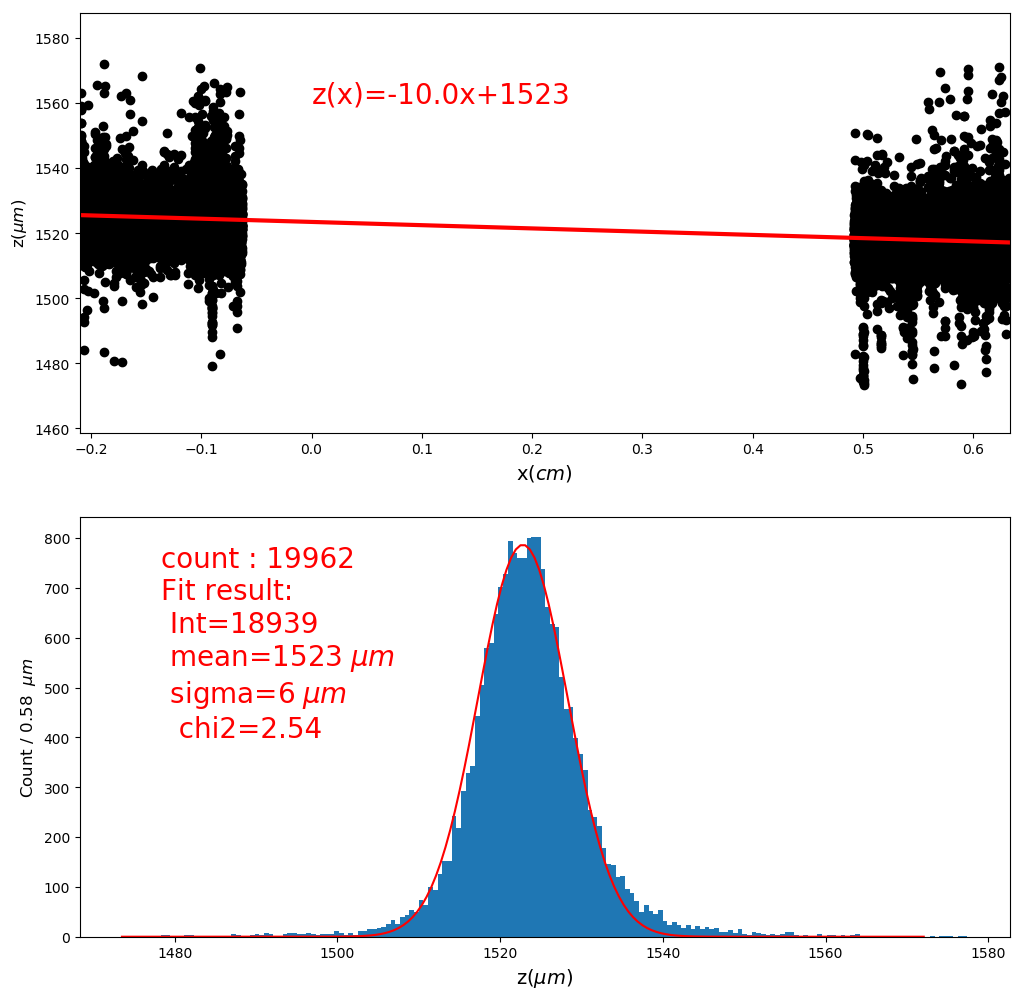
\includegraphics[width=0.8\textwidth,keepaspectratio]{marble.png}
            \caption[Calibration du système de mesure CCI]{\label{fig::marbre}Calibration de la planéité du marbre. Le graphe du haut montre la pente du marbre le long de l'axe de mesure $x$, le graphe du bas montre la dispersion de l'épaisseur du marbre après correction de la pente autour de $x=0$.}
%            \begin{minipage}{0.56\textwidth}
%              \begin{subfigure}[t]{\textwidth}
%                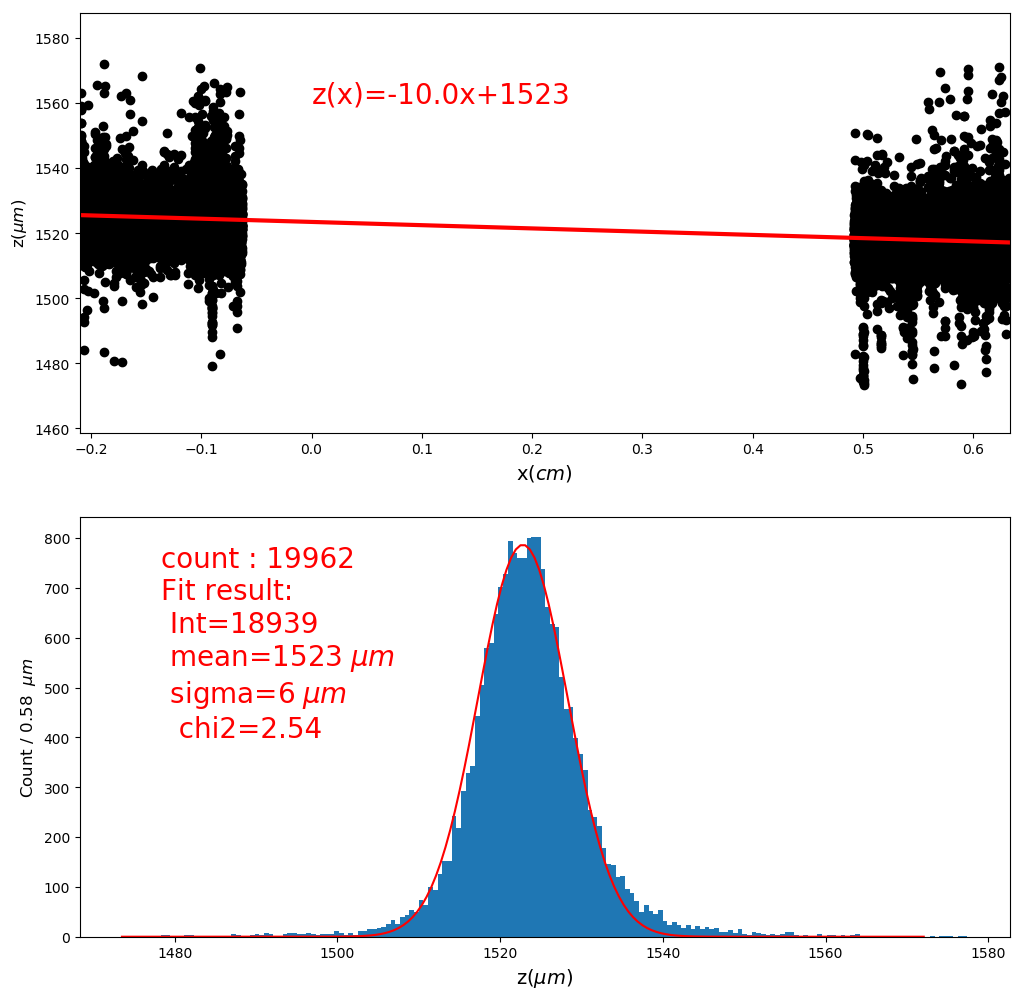
\includegraphics[width=\textwidth,keepaspectratio]{marble.png}
%                \caption{\label{fig::marbre}Calibration du marbre. Le graph du haut montre la pente du marbre le long de l'axe de mesure $x$, le graph du bas montre la dispersion de l'épaisseur du marbre après correction de la pente autour de $x=0$. \textcolor{red}{Je referai ces plots en plus lisible}}
%              \end{subfigure}
%            \end{minipage}
%            \hfill
%            \begin{minipage}{0.38\textwidth}
%              \begin{subfigure}[t]{\textwidth}
%                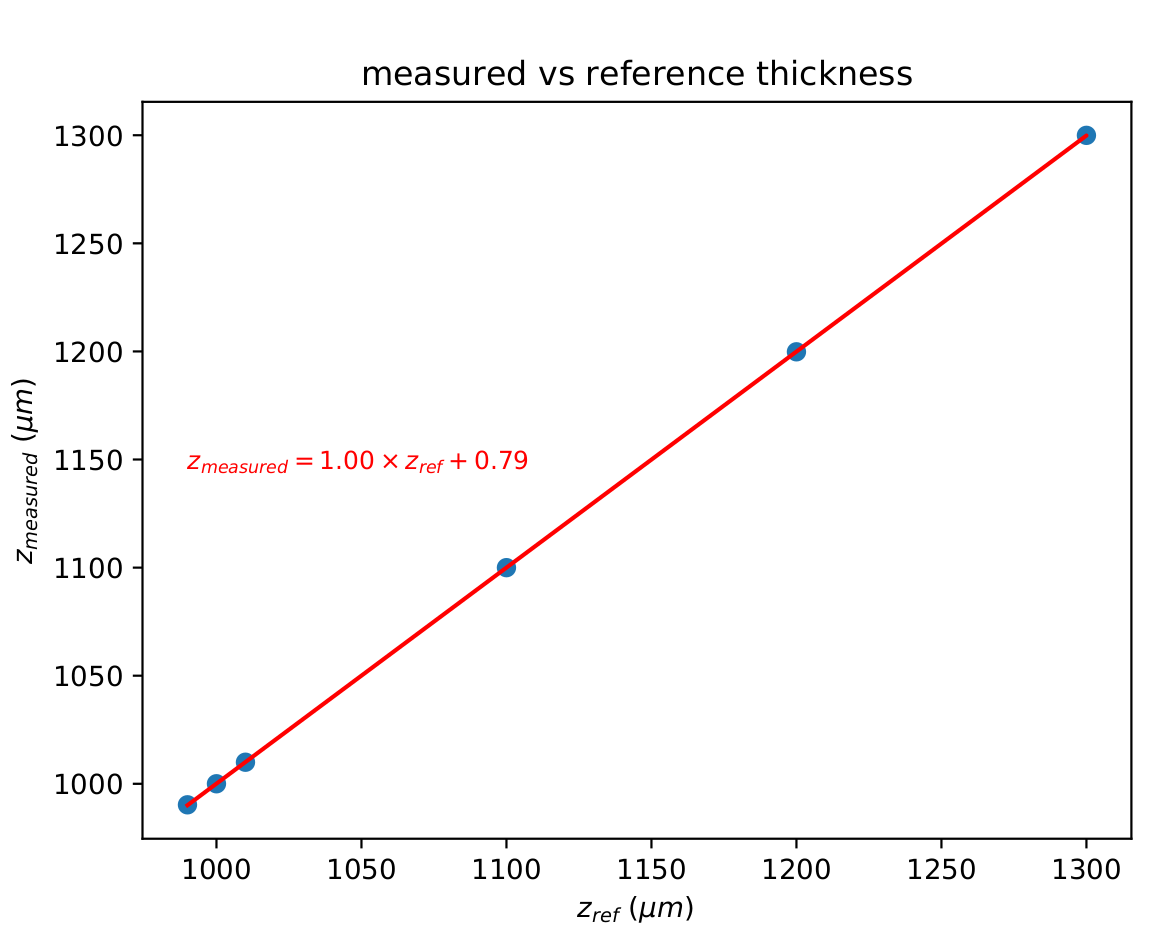
\includegraphics[width=\textwidth,keepaspectratio]{optic_response.png}
%                \caption{\label{fig::optic_response}Calibration de la réponse du crayon optique avec six cales de différentes épaisseurs.}
%              \end{subfigure}
%              \begin{subfigure}[t]{\textwidth}
%                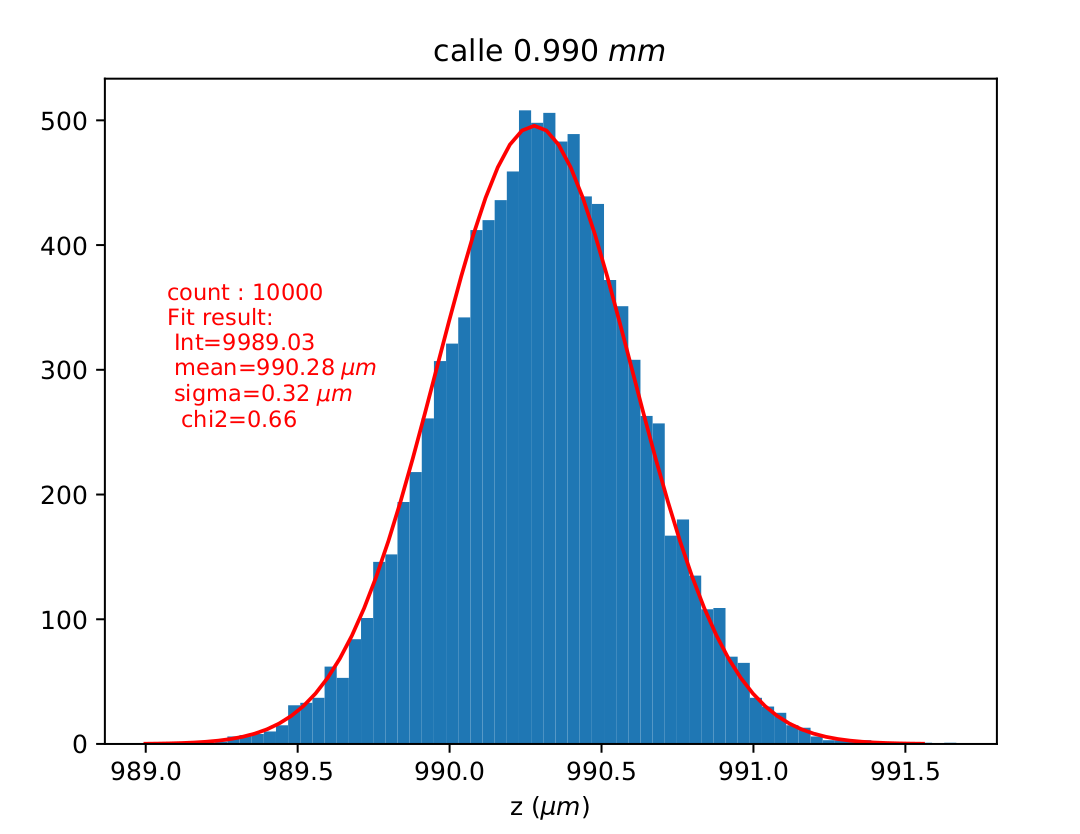
\includegraphics[width=\textwidth,keepaspectratio]{calle.png}
%                \caption{\label{fig::calle}Dispersion de l'épaisseur mesurée d'une cale de \SI{0.99}{\milli\meter}.}
%              \end{subfigure}
%            \end{minipage}
%            \caption[Calibration du système de mesure \gls{cci}.]{\label{fig::calibration}Calibration du système de mesure \gls{cci}.}
          \end{figure}
          Le mouvement selon l'axe $y$ ne peut se faire qu'en déplaçant manuellement la poutre, aussi les mesures ont été prises ligne par ligne. Les mesures sont corrigées pour l'inclinaison du marbre, mesurée à chaque ligne. Celui-ci présentait une pente autour de $\SI{10}{\micro\meter\per\meter}$ (\autoref{fig::marbre}). La moyenne de la distribution des hauteurs du marbre corrigée pour la pente servait de zéro pour les mesures des épaisseurs du \gls{lem} lui même. La réponse du dispositif optique à la hauteur à mesurer a également été calibrée avec des cales d'épaisseur allant de $\SI{900}{\micro\meter}$ à $\SI{1300}{\micro\meter}$.
% en ajustant une droite d'équation $z_{mesure} = \alpha \cdot z_{cale} + \beta$ à la hauteur $z_{mesure}$ mesurée contre la hauteur $z_{cale}$ indiquée sur la cale. Le coefficient $\alpha$ est de $1.00$ et le coefficient $\beta$ de $\SI{0.72}{\micro\meter}$.
          
      \subsubsection{Résultats}\label{sec::thickness_result}
         
        \begin{figure}[htpb]
          \centering
          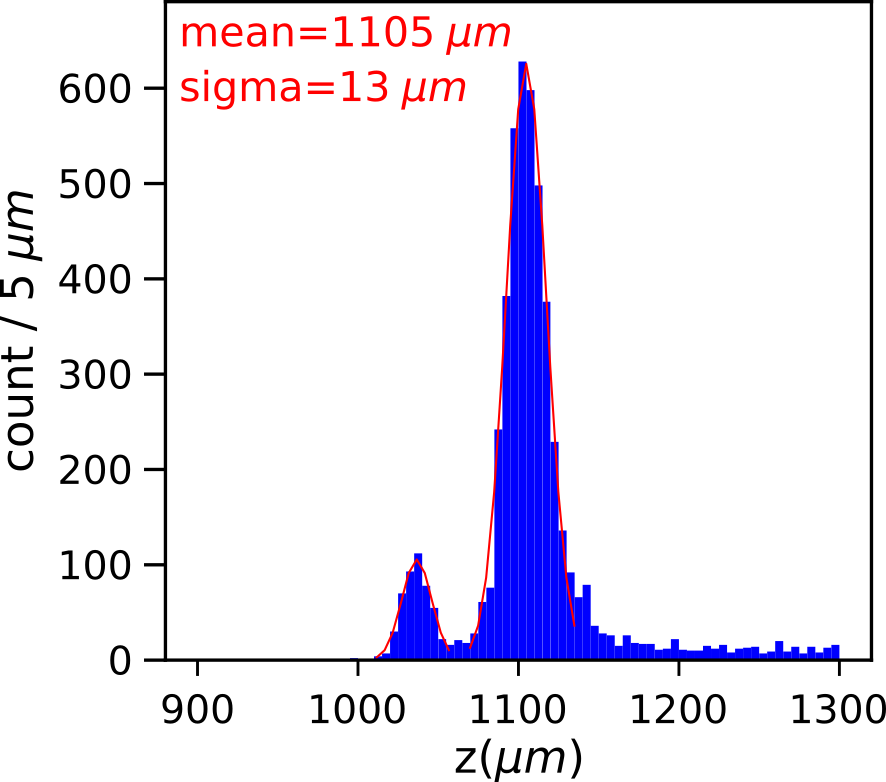
\includegraphics[width=0.7\textwidth,keepaspectratio]{distri_1_trou_lem.png}
          \caption[Exemple de mesure de l'épaisseur d'un LEM]{\label{fig::distri_1_trou_lem}Exemple de mesure de l'épaisseur d'un \gls{lem} à travers un trou de la plaque en acier. Le petit pic de gauche correspond à la lumière réfléchie par le \gls{fr4} du RIM, le pic de droite correspond à la lumière réfléchie par le cuivre.}
        \end{figure}
        \begin{figure}[htpb]
          \centering
          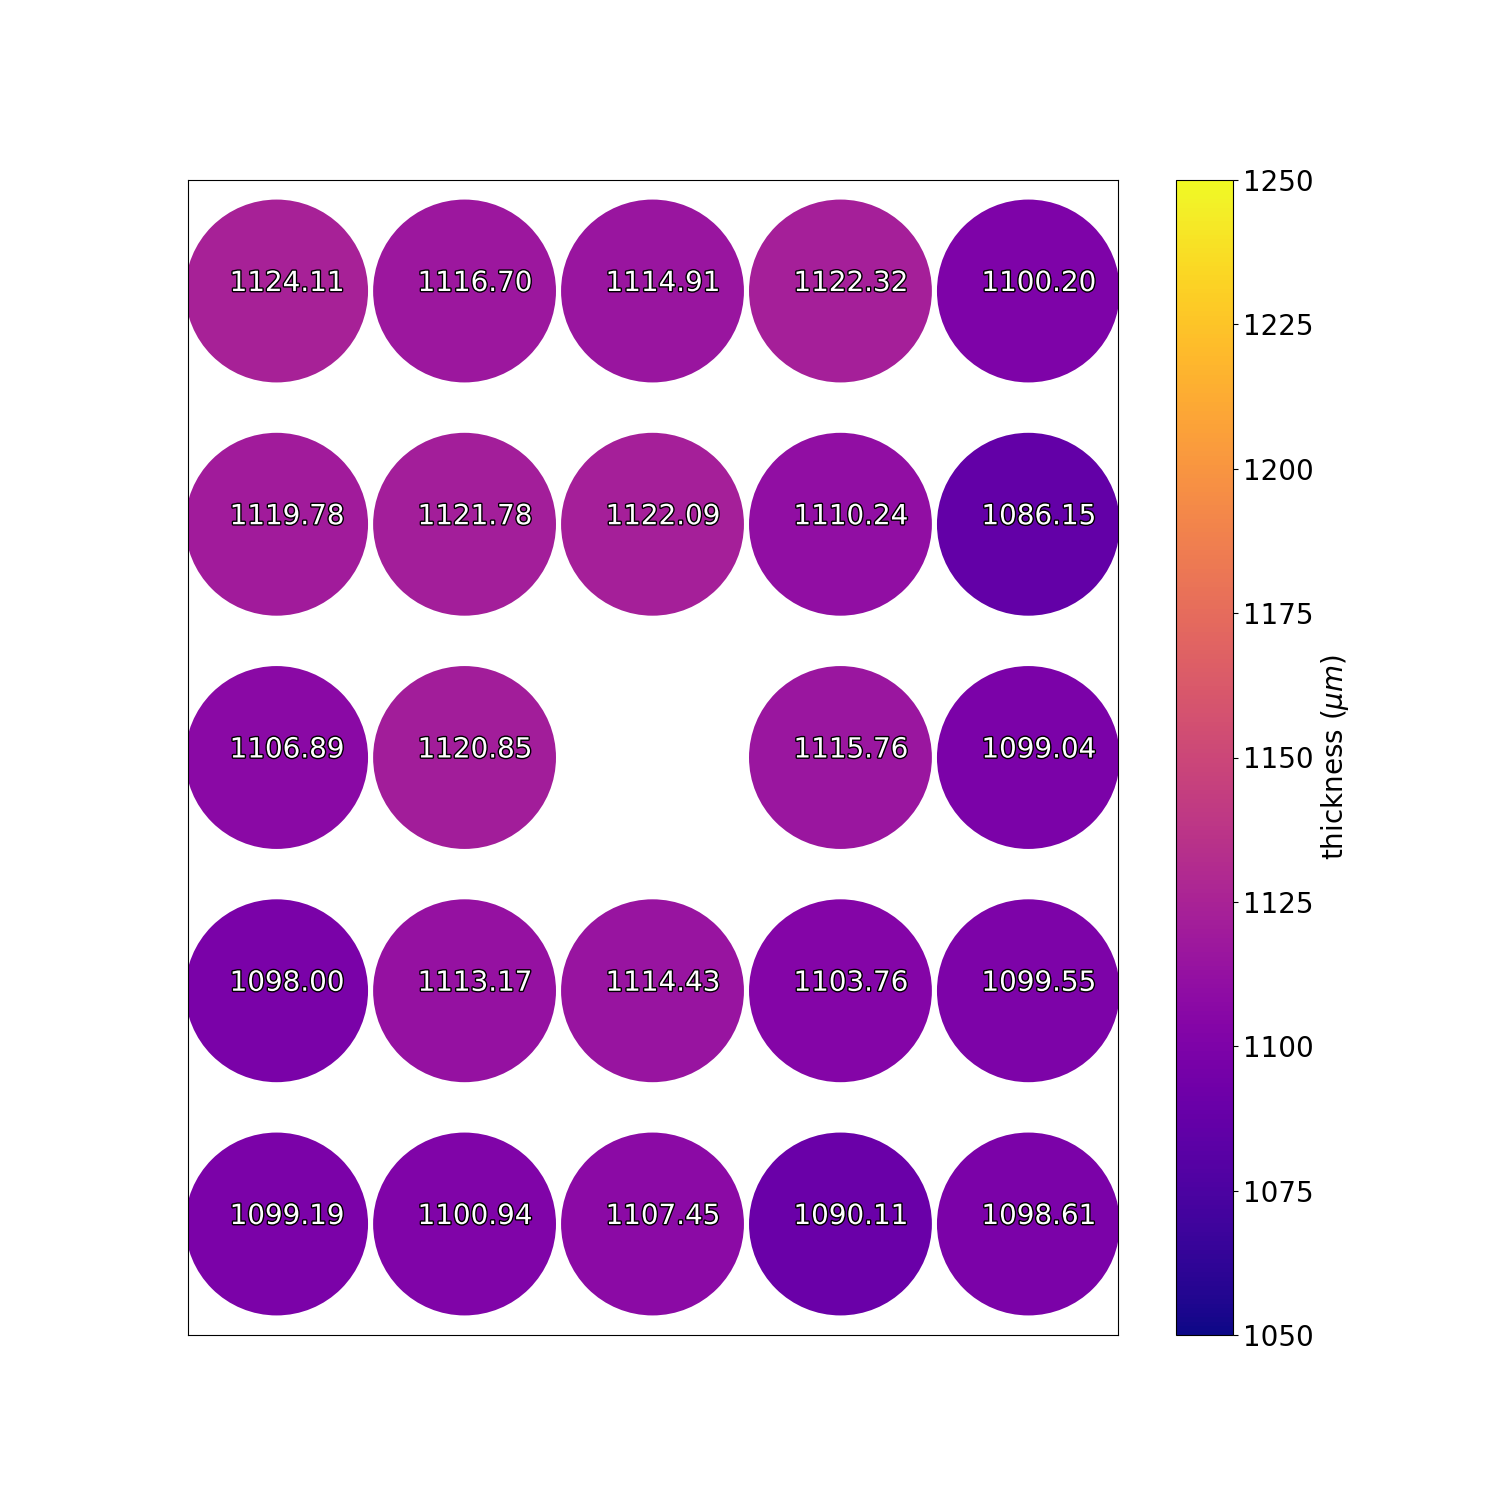
\includegraphics[width=0.5\textwidth,keepaspectratio]{2D_LEM_thickness_distri.png}
          \caption[Uniformité de l'épaisseur d'un LEM]{\label{fig::distri_24_trou_lem_2D}Uniformité de l'épaisseur d'un \gls{lem} mesurée à travers les 24 trous de la plaque d'acier.}
        \end{figure}
          
        \begin{figure}[htpb]
%          \hfill
%          \begin{subfigure}[t]{0.48\textwidth}
%            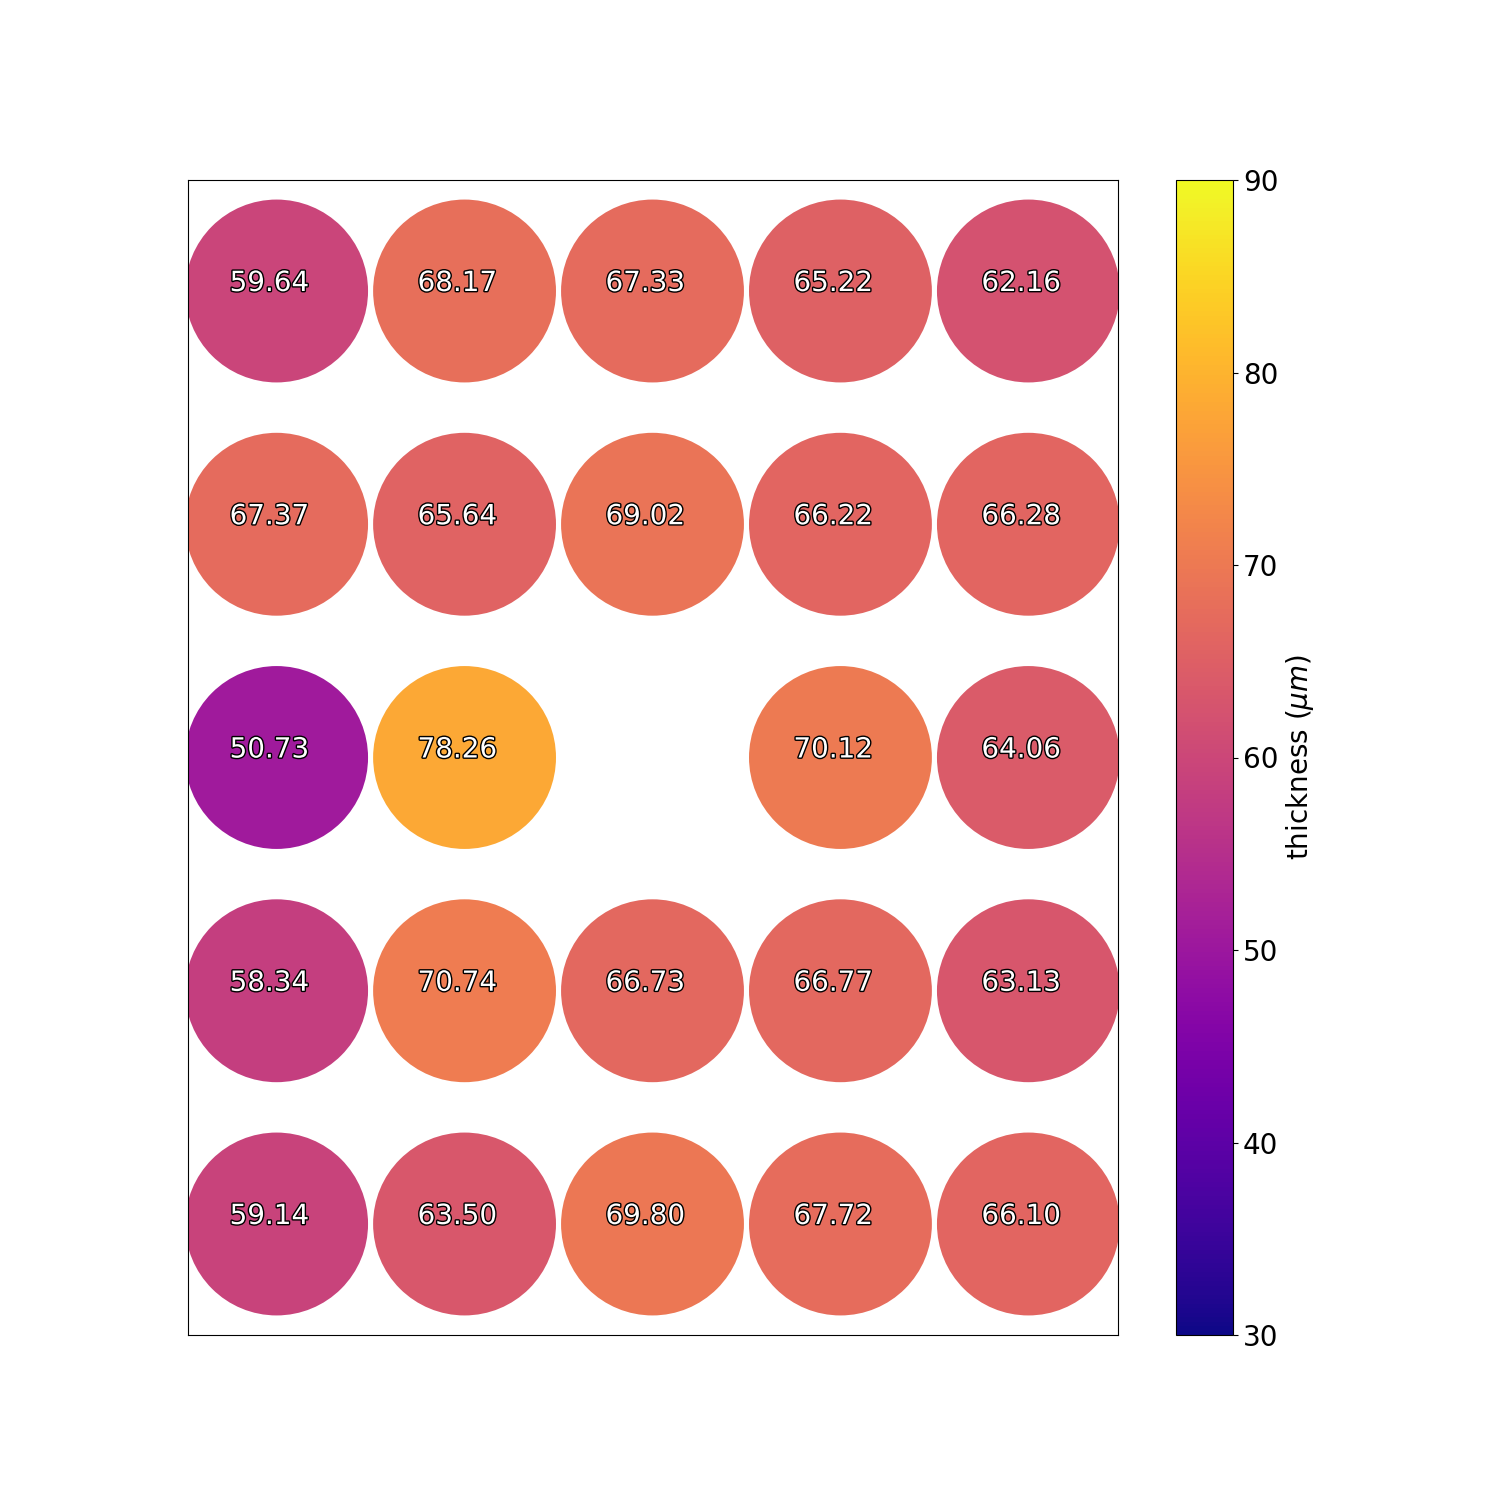
\includegraphics[width=\textwidth,keepaspectratio]{2D_copper_thickness_distri.png}
%            \caption{\label{fig::distri_24_trou_cuivre_2D}Visualisation de la variation d'épaisseur de cuivre d'un \gls{lem} mesurée à travers les 24 trous de la plaque d'acier.}
%          \end{subfigure}\\
          \begin{subfigure}[b]{0.48\textwidth}
            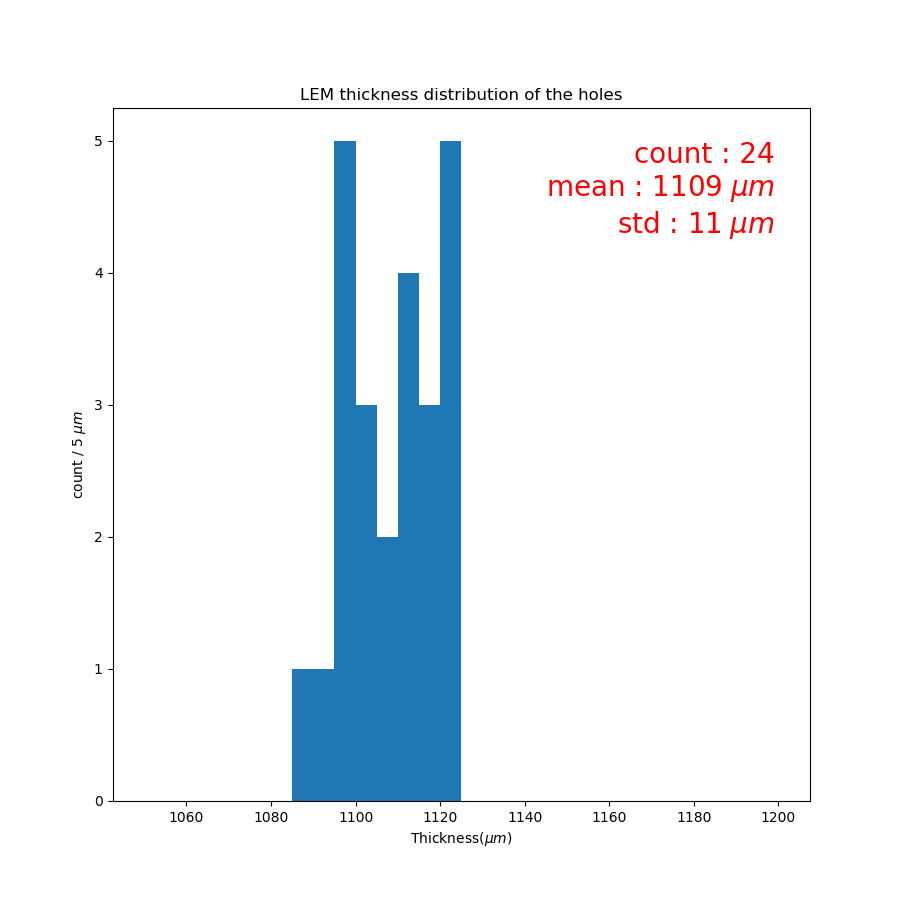
\includegraphics[width=\textwidth,keepaspectratio]{LEM.png}
            \caption{\label{fig::distri_24_trou_lem_1D}Distribution de l'épaisseur totale d'un \gls{lem} mesurée à travers les 24 trous de la plaque d'acier.}
          \end{subfigure}
          \hfill
          \begin{subfigure}[b]{0.48\textwidth}
            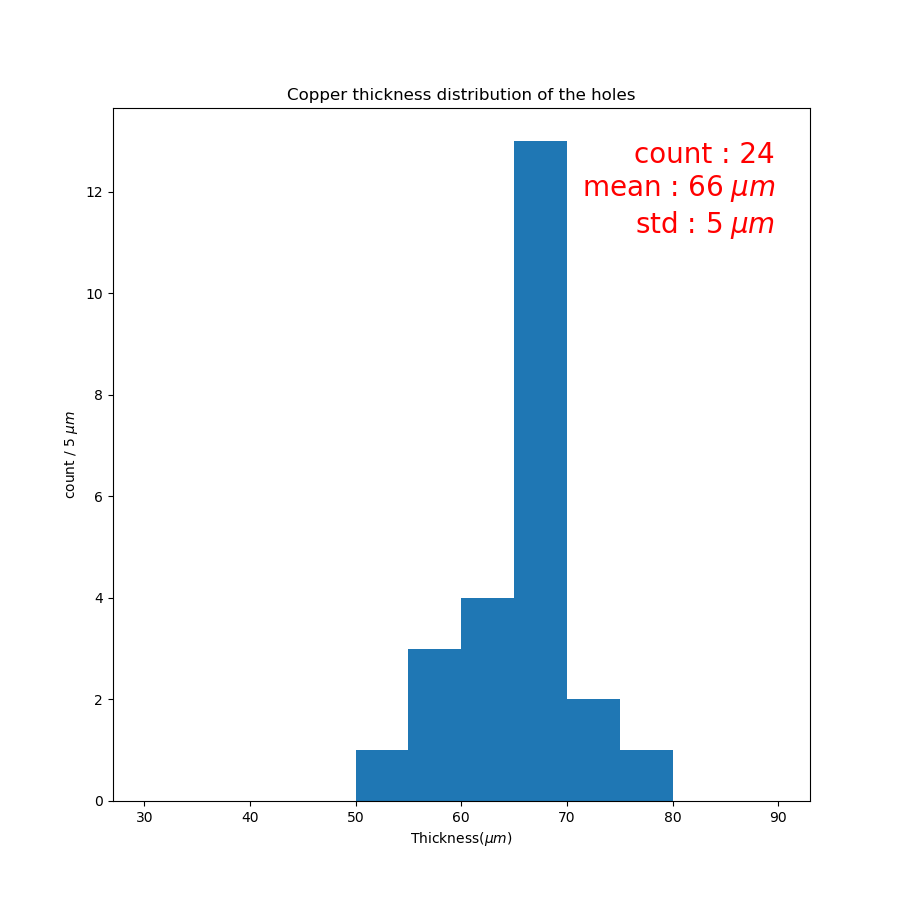
\includegraphics[width=\textwidth,keepaspectratio]{Copper.png}
            \caption{\label{fig::distri_24_trou_cuivre_1D}Distribution de l'épaisseur de cuivre d'un \gls{lem} mesurée à travers les 24 trous de la plaque d'acier.}
          \end{subfigure}
          \caption[Résultats des mesures d'épaisseur pour un LEM]{\label{fig::distri_epaisseur_1_lem}Résultats des mesures d'épaisseur pour un \gls{lem}.}
        \end{figure}
                
        \begin{figure}[htpb]
          \begin{subfigure}[t]{0.48\textwidth}
            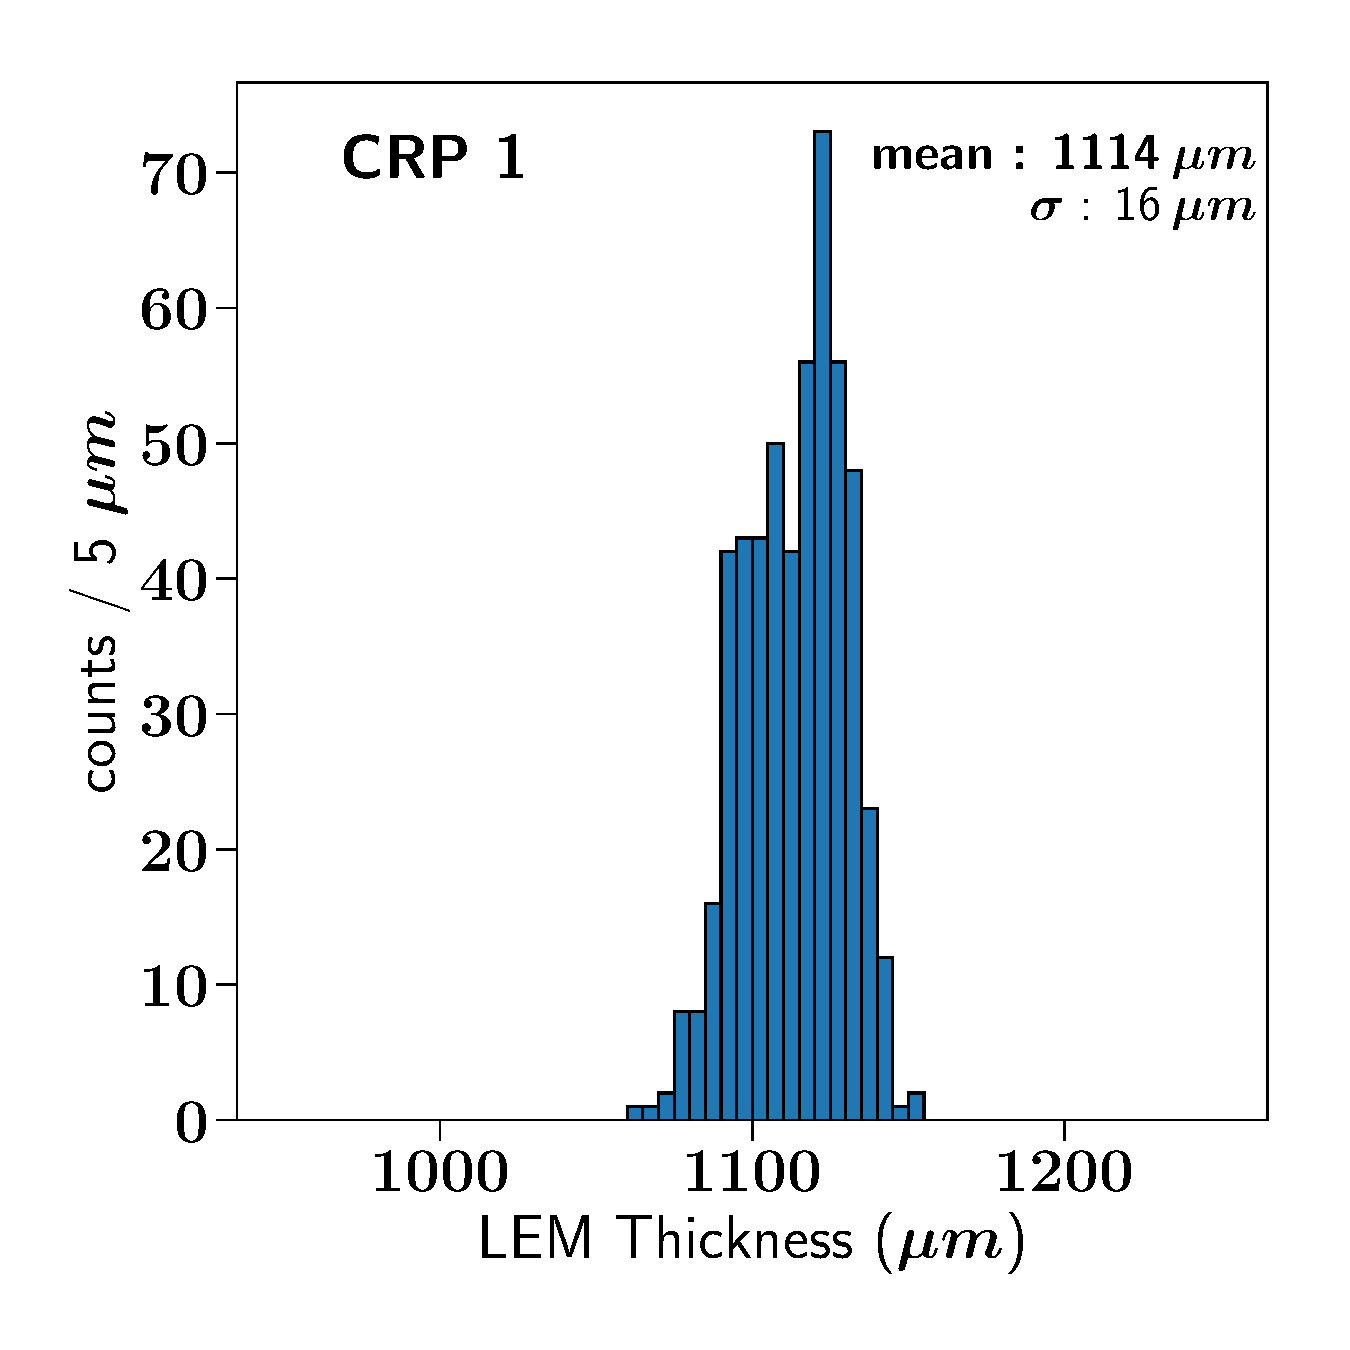
\includegraphics[width=\textwidth,keepaspectratio]{LEM_sum_all_histo_Saclay.pdf}
            \caption{\label{fig::distri_lem_saclay}Distribution de l'épaisseur totale de tous les \glspl{lem} du \gls{crp} 1 du démonstrateur \SSS{} mesurée à travers les 24 trous de la plaque d'acier.}
          \end{subfigure}
          \hfill
          \begin{subfigure}[t]{0.48\textwidth}
            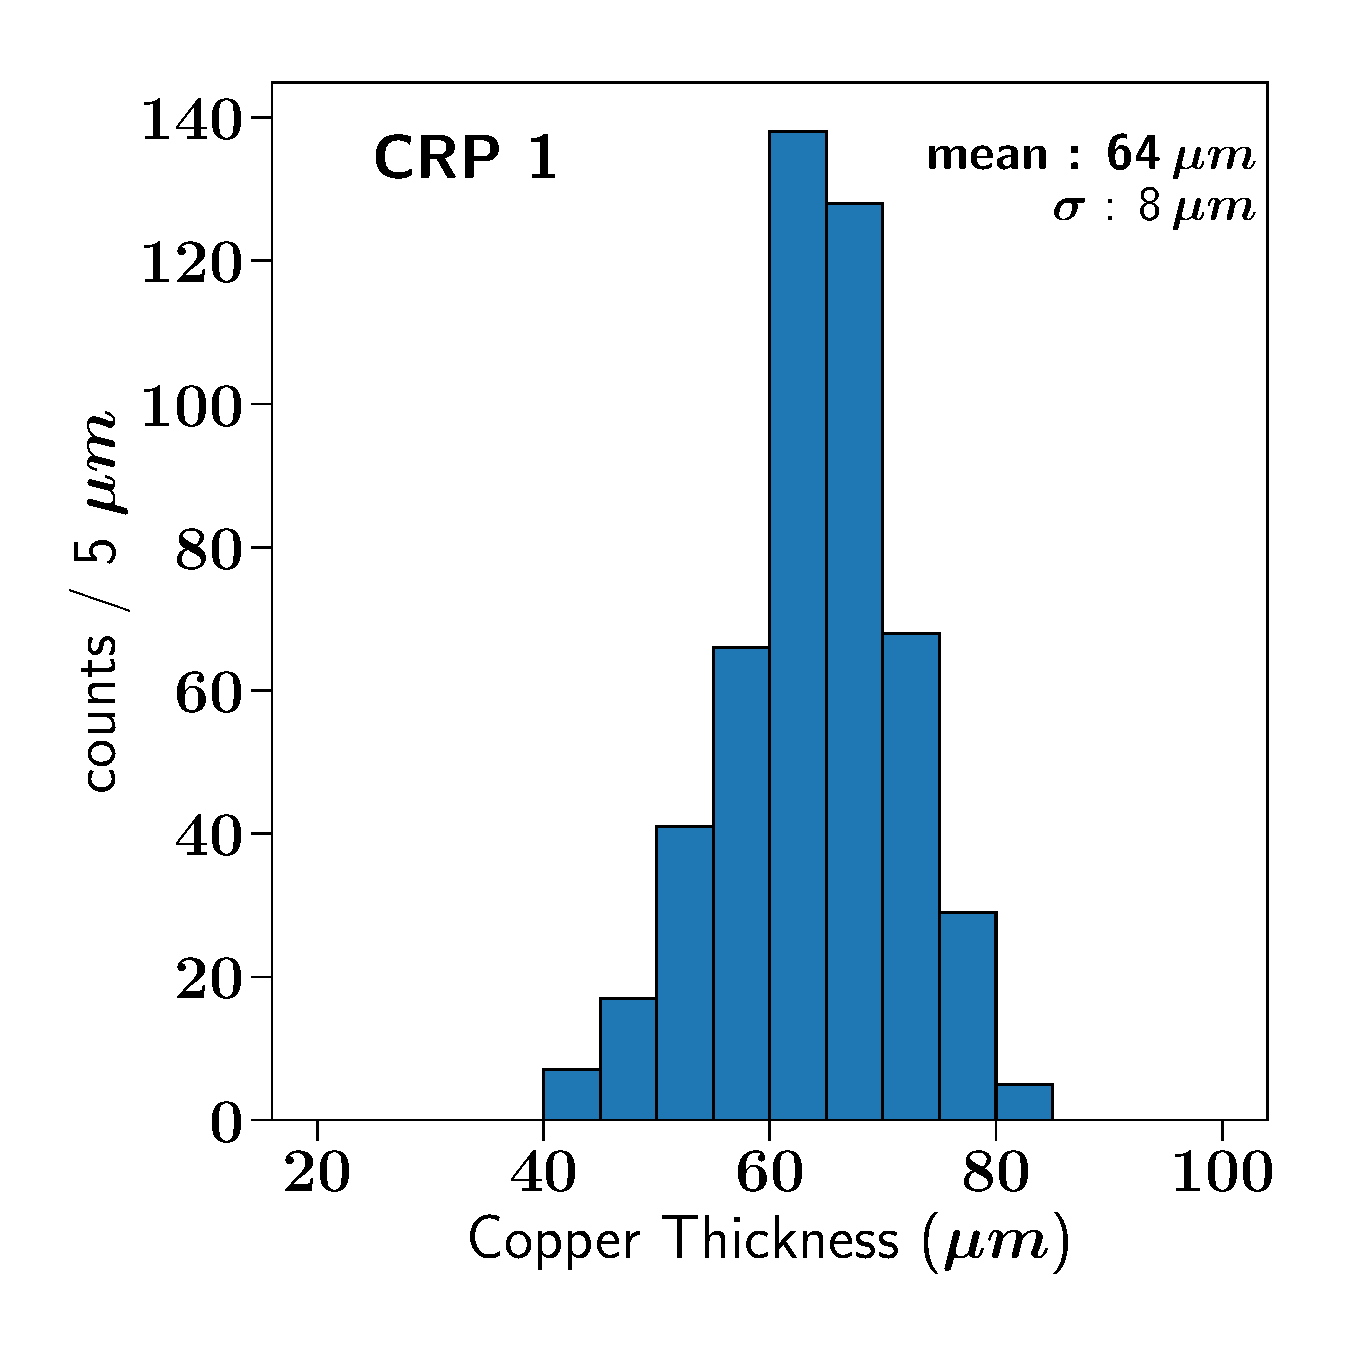
\includegraphics[width=\textwidth,keepaspectratio]{Copper_sum_all_histo_Saclay.pdf}
            \caption{\label{fig::distri_cuivre_saclay}Distribution de l'épaisseur de cuivre de tous les \glspl{lem} du \gls{crp} 1 du démonstrateur \SSS{} mesurée à travers les 24 trous de la plaque d'acier.}
          \end{subfigure}\\
          \begin{subfigure}[b]{0.48\textwidth}
            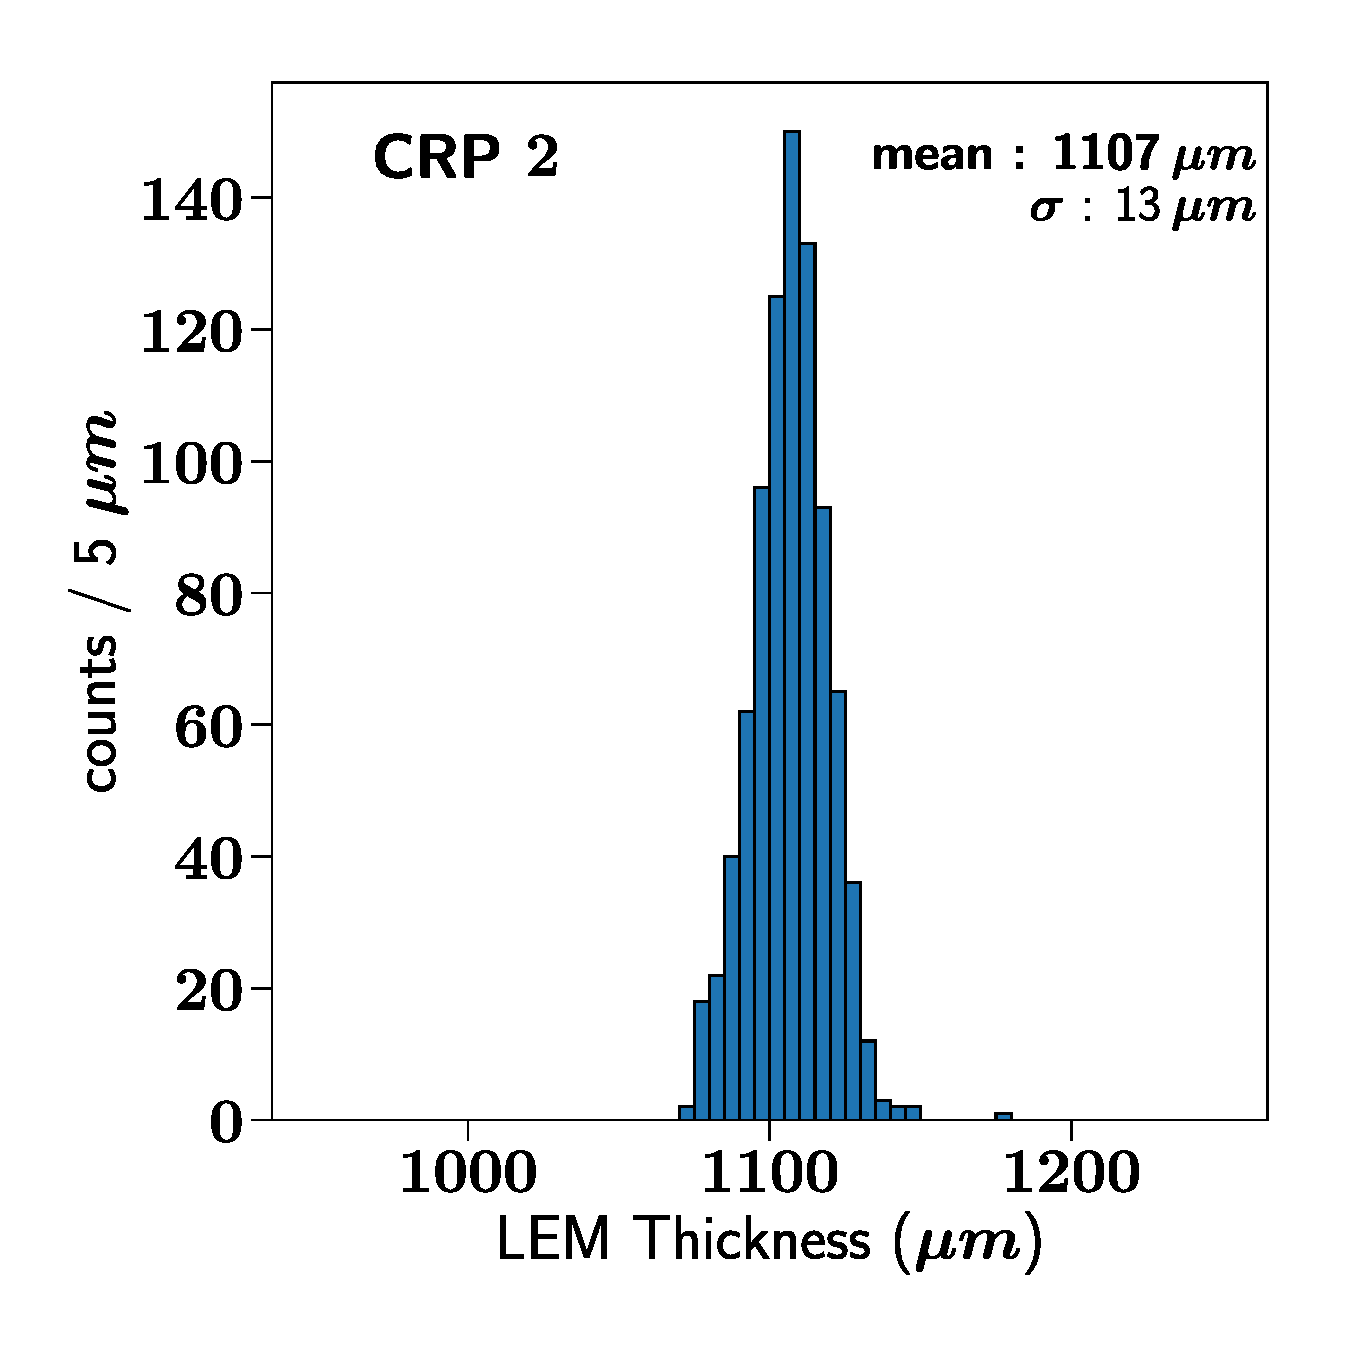
\includegraphics[width=\textwidth,keepaspectratio]{LEM_sum_all_histo_CERN.pdf}
            \caption{\label{fig::distri_lem_cern}Distribution de l'épaisseur totale de tous les \glspl{lem} du \gls{crp} 2 du démonstrateur \SSS{} mesurée à travers les 24 trous de la plaque d'acier.}
          \end{subfigure}
          \hfill
          \begin{subfigure}[b]{0.48\textwidth}
            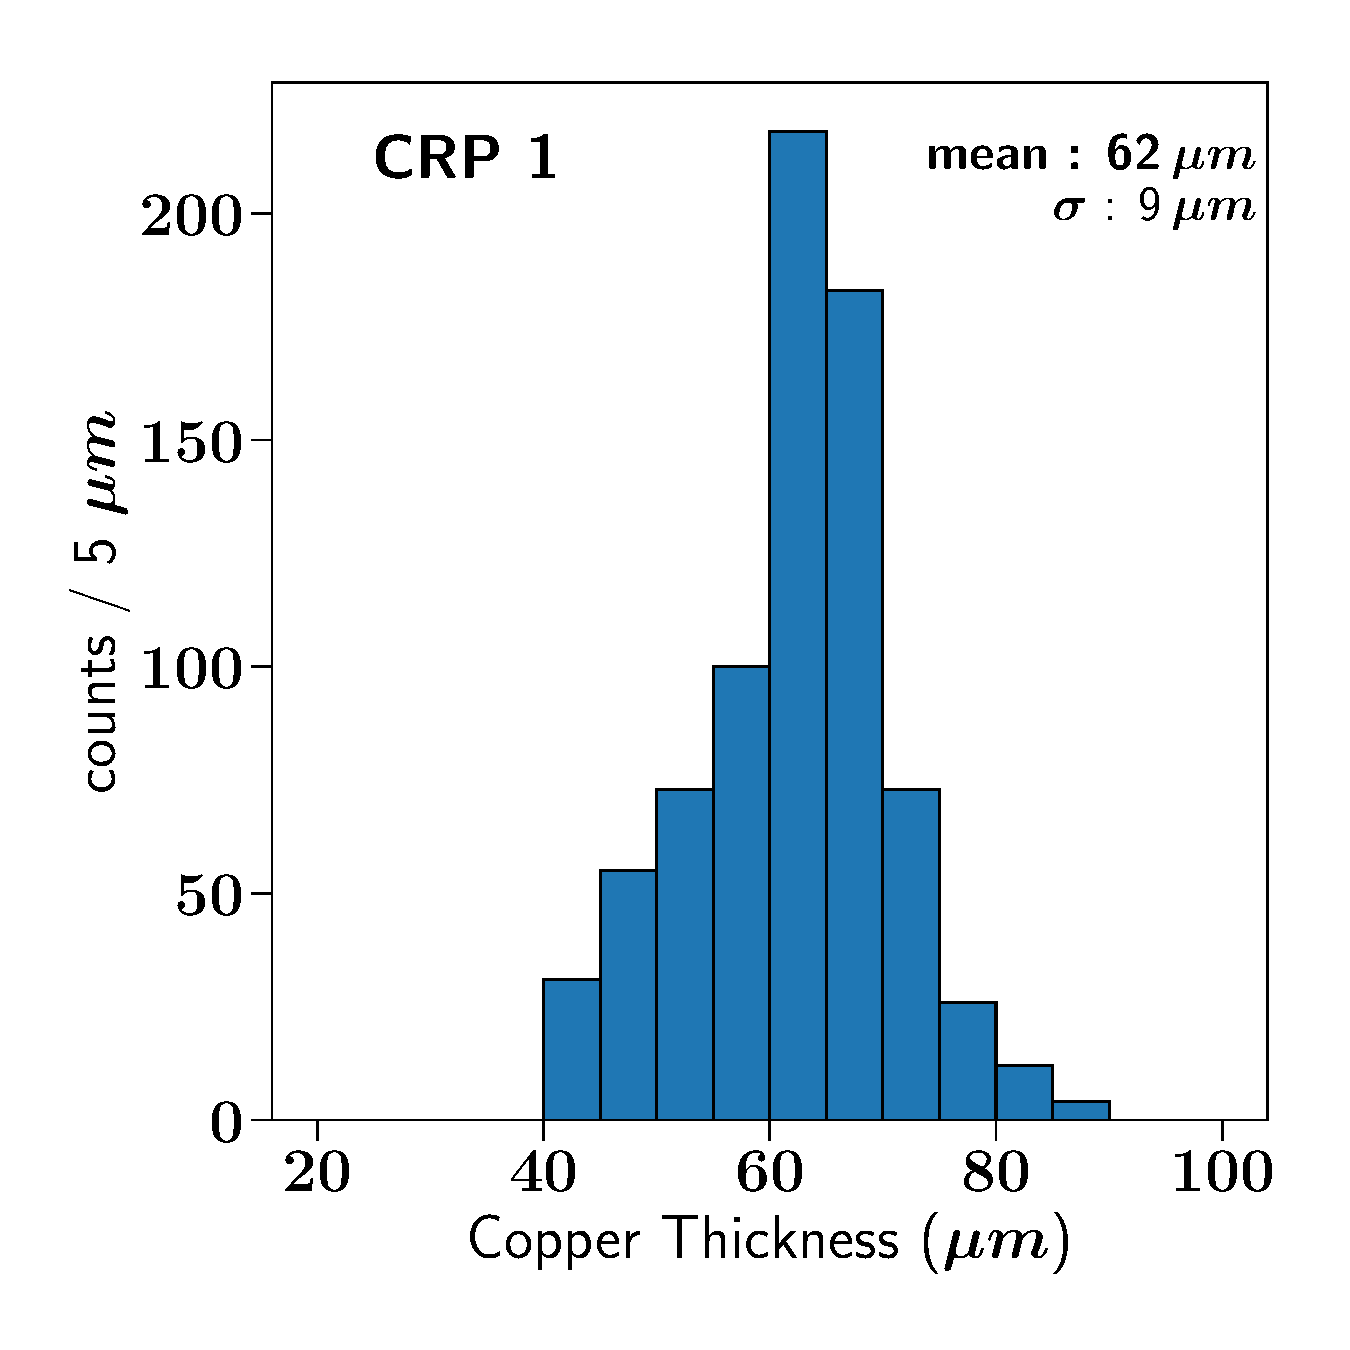
\includegraphics[width=\textwidth,keepaspectratio]{Copper_sum_all_histo_CERN.pdf}
            \caption{\label{fig::distri_cuivre_cern}Distribution de l'épaisseur de cuivre de tous les \glspl{lem} du \gls{crp} 2 du démonstrateur \SSS{} mesurée à travers les 24 trous de la plaque d'acier.}
          \end{subfigure}
          \caption[Résultats des mesures d'épaisseur pour tous les LEM]{\label{fig::epaisseur_tous_lem}Résultats des mesures d'épaisseur pour tous les \glspl{lem}. La première ligne correspond aux \glspl{lem} du \gls{crp} 1 du démonstrateur \SSS{}, la seconde ligne correspond aux \glspl{lem} du \gls{crp} 2 du démonstrateur \SSS{}.}
        \end{figure}
                
%        \begin{figure}[htpb]
%          \begin{subfigure}[t]{0.48\textwidth}
%            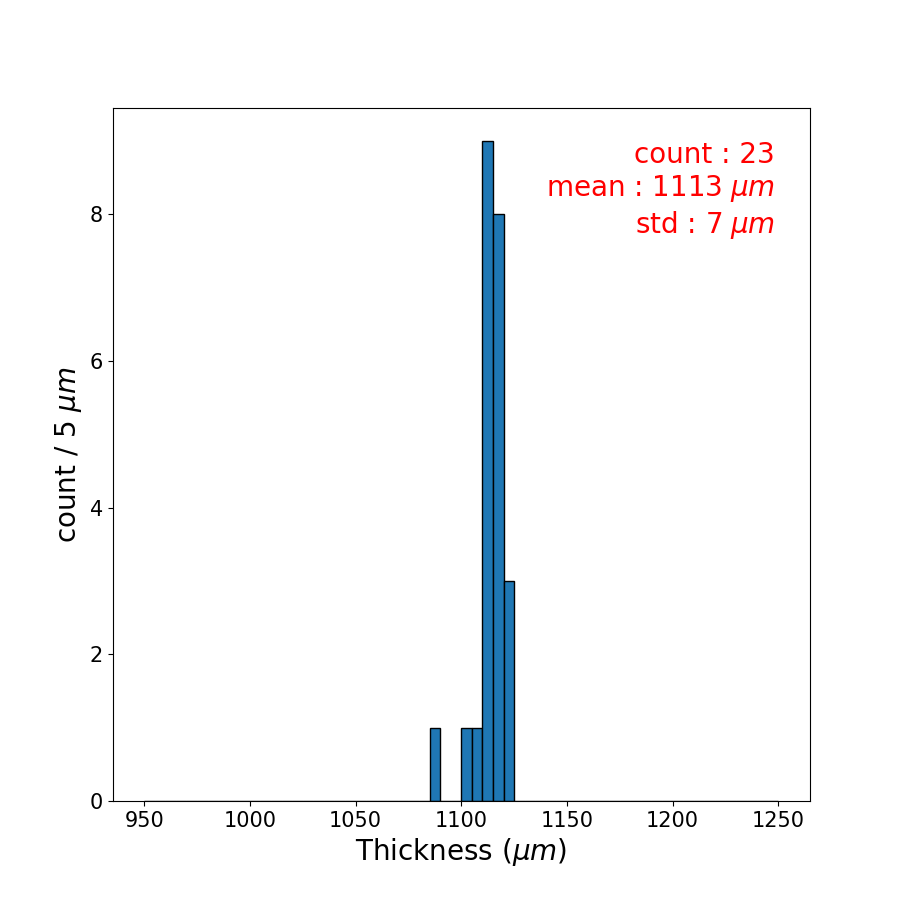
\includegraphics[width=\textwidth,keepaspectratio]{LEM_means_sum_all_histo_saclay.png}
%            \caption{\label{fig::distri_moyenne_lem_saclay}Distribution de l'épaisseur de totale moyennée sur les 24 trous de mesure d'un \gls{lem} pour tous les \glspl{lem} du \gls{crp} 1 du démonstrateur \SSS{}. Seuls \numprint{22} des \numprint{36} \glspl{lem} ont été mesurés.}
%          \end{subfigure}
%          \hfill
%          \begin{subfigure}[t]{0.48\textwidth}
%            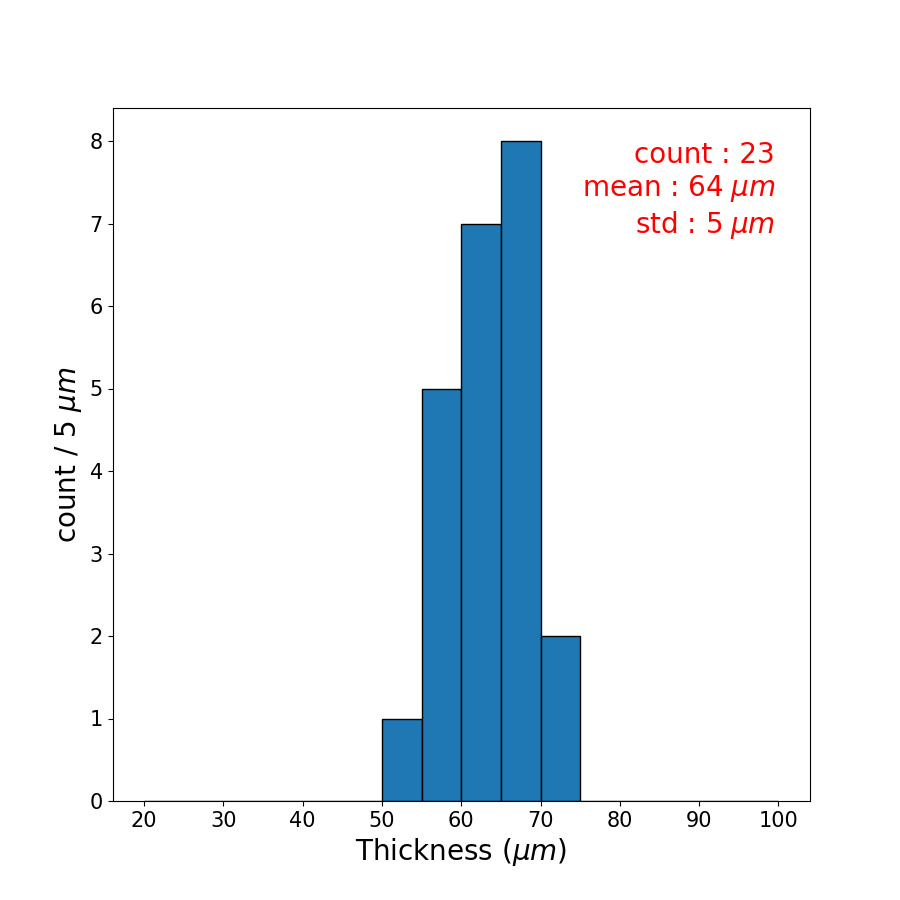
\includegraphics[width=\textwidth,keepaspectratio]{Copper_means_sum_all_histo_saclay.png}
%            \caption{\label{fig::distri_moyenne_cuivre_saclay}Distribution de l'épaisseur de cuivre moyennée sur les 24 trous de mesure d'un \gls{lem} pour tous les \glspl{lem} du \gls{crp} 1 du démonstrateur \SSS{}. Seuls \numprint{22} des \numprint{36} \glspl{lem} ont été mesurés}
%          \end{subfigure}\\
%          \begin{subfigure}[b]{0.48\textwidth}
%            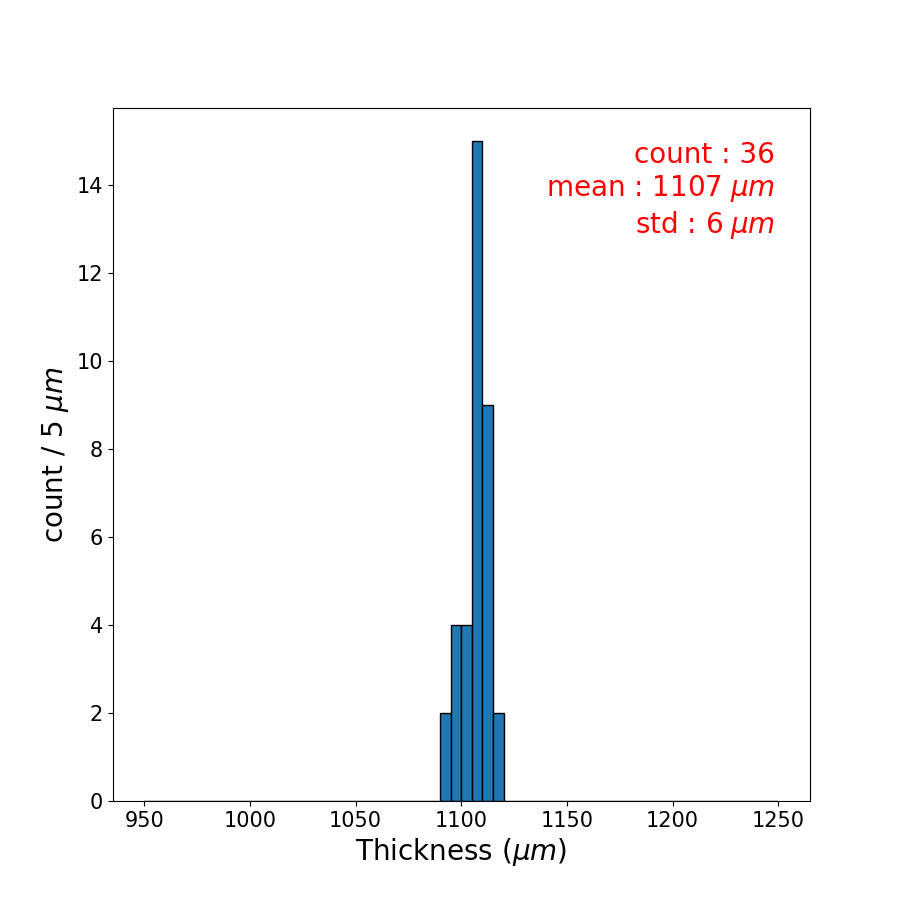
\includegraphics[width=\textwidth,keepaspectratio]{LEM_means_sum_all_histo_cern.png}
%            \caption{\label{fig::distri_moyenne_lem_cern}Distribution de l'épaisseur de totale moyennée sur les 24 trous de mesure d'un \gls{lem} pour tous les \glspl{lem} du \gls{crp} 2 du démonstrateur \SSS{}.}
%          \end{subfigure}
%          \hfill
%          \begin{subfigure}[b]{0.48\textwidth}
%            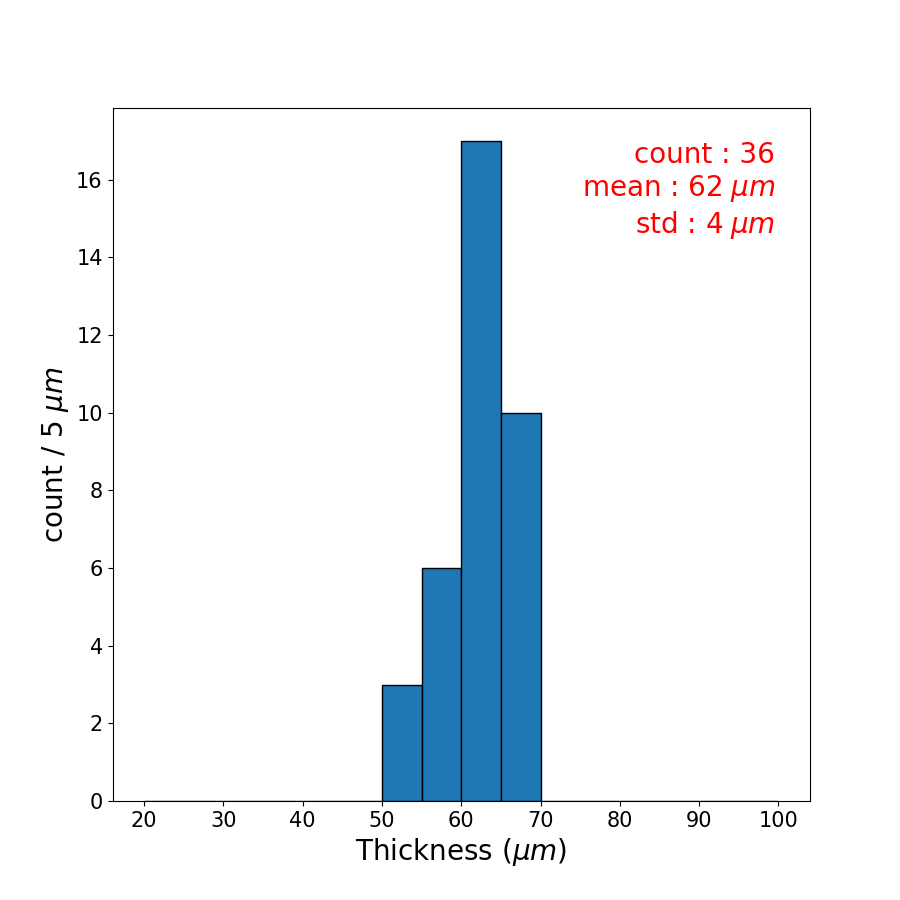
\includegraphics[width=\textwidth,keepaspectratio]{Copper_means_sum_all_histo_cern.png}
%            \caption{\label{fig::distri_moyenne_cuivre_cern}Distribution de l'épaisseur de cuivre moyennée sur les 24 trous de mesure d'un \gls{lem} pour tous les \glspl{lem} du \gls{crp} 2 du démonstrateur \SSS{}.}
%          \end{subfigure}
%          \caption[Résultats des mesures d'épaisseurs moyennées sur les 24 trous de mesure pour tous les \glspl{lem}.]{\label{fig::epaisseur_moyenne_tous_lem}Résultats des mesures d'épaisseur moyennée sur les 24 trous de mesure pour tous les \glspl{lem}. La première ligne correspond aux \glspl{lem} du \gls{crp} 1 du démonstrateur \SSS{}, la seconde ligne correspond aux \glspl{lem} du \gls{crp} 2 du démonstrateur \SSS{}.}
%        \end{figure}
            
        \begin{figure}[htbp]
          \centering
          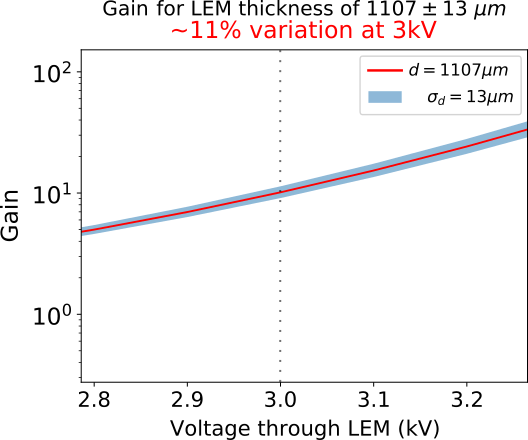
\includegraphics[width=0.8\textwidth,keepaspectratio]{measured_gain_fluctuations}
          \caption[Variation attendues du gain pour l'épaisseur moyennes des \glspl{lem} mesurés]{\label{fig::exp_gain_range}Variation attendue du gain pour une épaisseur de \gls{lem} de $\SI{1107}{\micro\meter}\pm\SI{13}{\micro\meter}$, d'après la formule \eqref{eq::townsend_avalanche_2} ajustée aux données du prototype de \threeL{}\cite{Cantini2014}.}
        \end{figure}
                
        Les distributions des hauteurs dans les 24 trous de mesure d'un \gls{lem} sont tracées avec correction pour la pente du marbre dans la \autoref{fig::distri_1_trou_lem}. Les pics sur les côtés des trous d'amplification étaient attendus, et sont dues une limitation de la technique \gls{cci} : certains rayons lumineux du crayon optique, qui ne sont pas focalisés sur la surface du \gls{fr4} et qui donc ne devraient pas être détectés, sont tout de même réfléchis par la paroi verticale en cuivre et sont détectés par le dispositif, faussant ainsi la distance mesurée. Ces pics, éliminés dans l'analyse, n'affectent pas la mesure de l'épaisseur totale. Les épaisseur de cuivre et de \gls{fr4} en revanche sont estimés à partir des quelques points de mesures pris sur la surface de \gls{fr4} des RIMs. La statistique étant faible sur cette surface il est possible que la mesure de l'épaisseur soit surestimée à cause de l'effet décrit plus haut. Les comparaisons aux mesures d'ELTOS semblent confirmer cette hypothèse, la technique \gls{cci} donnant un résultat plus grand d'environ \SI{10}{\micro\meter}. Cependant, ELTOS ne mesurant ces épaisseurs que sur les bords des \glspl{lem}, il est également possible que l'épaisseur de cuivre ne soit pas identique au milieux et au bord.
                
        Une double gaussienne est ajustée sur la distribution montrée en \autoref{fig::distri_1_trou_lem} afin de déterminer l'épaisseur totale $E_T$ du \gls{lem} ainsi que l'épaisseur $E_C$ du cuivre. La moyenne de la gaussienne la plus à droite sur la \autoref{fig::distri_1_trou_lem} correspond à l'épaisseur totale $E_T$ du \gls{lem}, tandis que la moyenne de la gaussienne la plus à gauche correspond à $E_T - E_C$, en supposant que l'épaisseur du cuivre est la même sur chaque face. $E_C$ est alors calculable facilement, de même que l'épaisseur de \gls{fr4} $E_F$ car nous avons la relation $E_T = E_F + 2E_C$.
                
        A noter que les mesures ne permettaient pas toujours de d'ajuster deux gaussiennes. Dans certains cas, seul l'épaisseur totale était accessible, il y a donc moins de statistiques dans les histogrammes des épaisseurs de cuivre et de \gls{fr4}.
                
        La \autoref{fig::distri_epaisseur_1_lem} montre les distributions de l'épaisseur totale et de l'épaisseur de cuivre pour les 24 trous de mesure d'un \gls{lem}. La \autoref{fig::distri_24_trou_lem_2D} montre l'uniformité de l'épaisseur totale d'un \gls{lem}. La comparaison de cette uniformité entre plusieurs \glspl{lem} permet de voir si des zones semblent toujours être plus hautes ou plus basses. De tels zones n'ont pas été observées.
                
        Afin d'estimer les variations attendues du gain sur les deux \glspl{crp} du démonstrateur \SSS{}, la distribution des épaisseurs dans chaque trou de mesure des \glspl{lem} de chaque \gls{crp} est montrée en \autoref{fig::epaisseur_tous_lem}. La \autoref{fig::exp_gain_range} montre les variations attendues du gain pour une épaisseur de \gls{lem} de $\SI{1107}{\micro\meter}\pm\SI{13}{\micro\meter}$, correspondant 36 \glspl{lem} produits par le \gls{cern} (\gls{crp} 2). À \SI{3.1}{\kilo\volt}, la variation est de l'ordre de $15\%$. On peut de plus remarquer qu'en utilisant les ajustements aux données du prototype de \threeL{}, le gain à \SI{3.1}{\kilo\volt} est inférieur à 20. Ceci est due au fait que l'épaisseur totale des \glspl{lem} est autour de \SI{1107}{\micro\meter}, au lieu des \SI{1080}{\micro\meter} des \glspl{lem} du \threeL{}. À même tension, le champ d'amplification est donc plus faible. Les mesures du \SSS{} vérifieront cette valeur de gain, qui est très sensible au valeurs obtenues pour les coefficients $A$ et $B$ de la formule \eqref{eq::townsend_avalanche_2}.
                
%        La \autoref{fig::epaisseur_moyenne_tous_lem} montre la distributions des épaisseurs totales et des épaisseurs de cuivre moyennées sur les 24 trous de chaque \gls{lem} pour les deux \gls{crp}. Elle permet de comparer nos mesures à celles d'ELTOS, qui ne réalisait que 2 mesures par \gls{lem} pour l'épaisseur de cuivre et 4 pour l'épaisseur totale. 
                
      \subsubsection{Comparaison aux mesures faites par ELTOS}\label{sec::thickness_comparison_eltos}
            
        \begin{figure}[htpb]
          \begin{subfigure}[t]{0.68\textwidth}
            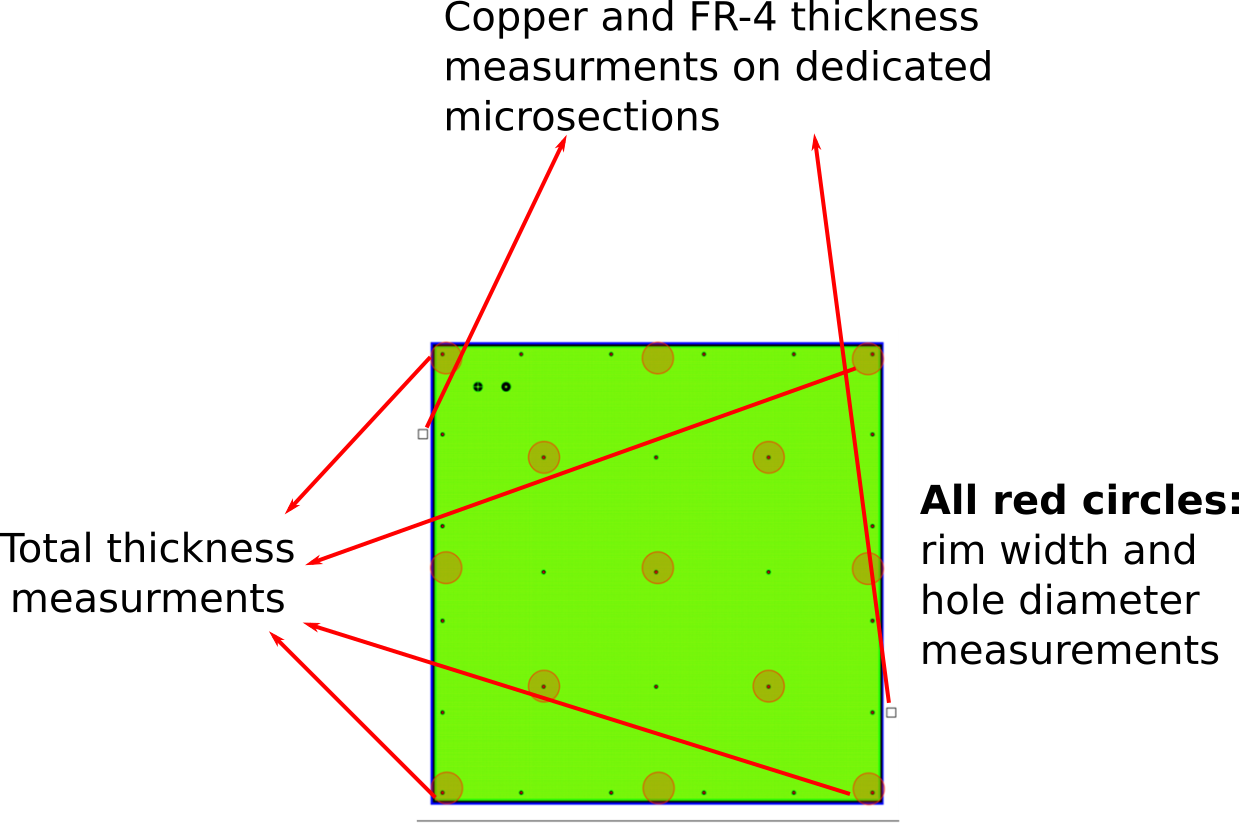
\includegraphics[width=\textwidth]{eltos_measurement.png}
            \caption{Gerber d'un \gls{lem} avec indiquées en rouge les zones de mesure des caractéristiques géométriques pour vérification de la concordance au cahier des charges présenté en \autoref{sec::LEM}. Deux échantillons de surface de \gls{lem} étaient prévues dans le gerber pour y effectuer des mesures d'épaisseur.}
          \end{subfigure}
          \hfill
          \begin{subfigure}[t]{0.3\textwidth}
            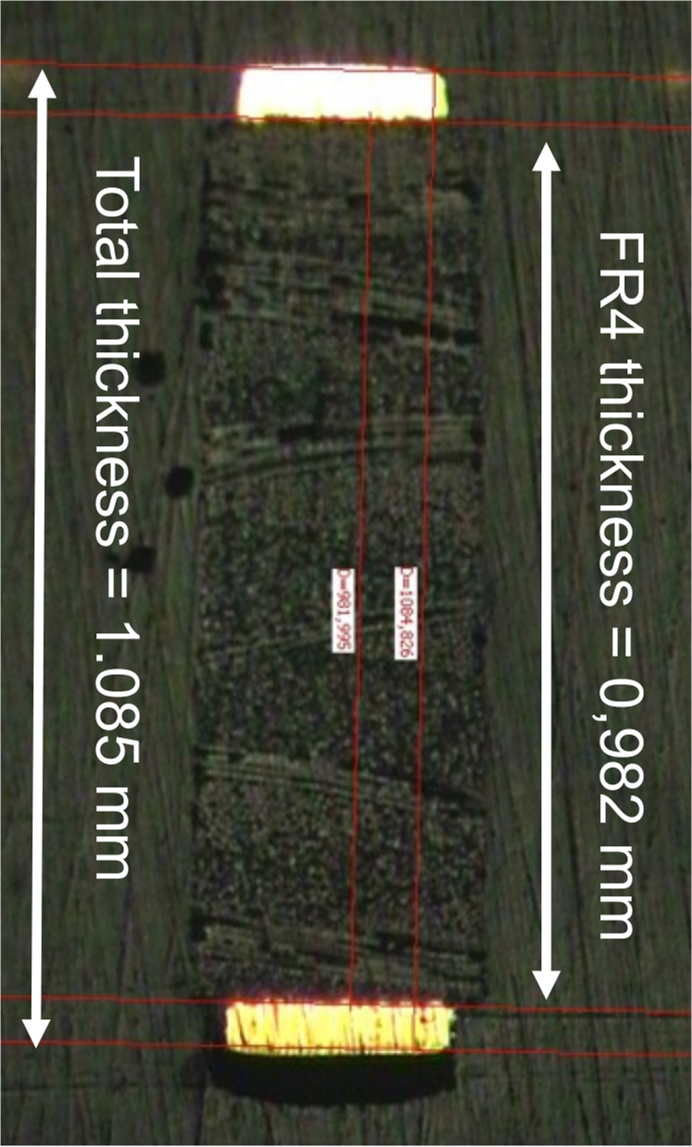
\includegraphics[width=\textwidth]{microsection_thickness.png}
            \caption{\label{fig::microsection}Vue d'un échantillon de surface au microscope où l'on peut voir les mesures d'épaisseur de \gls{fr4} et de cuivre.}
          \end{subfigure}
          \caption[Zones de mesuredes caractéristiques géométriques d'un LEM par ELTOS]{\label{fig::mesures_eltos}zones de mesure des caractéristiques géométriques d'un \gls{lem} par ELTOS}
        \end{figure}
            
        La \autoref{fig::mesures_eltos} montre les zones du \gls{lem} où ELTOS a mesuré les différentes caractéristiques géométriques : la taille totale, l'épaisseur totale, l'épaisseur de cuivre, l'épaisseur de \gls{fr4}, l'épaisseur des RIMs et le diamètre des trous. Les épaisseurs de cuivre et de \gls{fr4} étaient mesurées au microscope sur un des deux échantillons de surface de \gls{lem} prévus dans le gerber à cet effet, donnant une statistique de 72 pour les moyennes et écarts type de chaque \gls{crp} du démonstrateur \SSS{}. L'épaisseur totale était mesurée à 10 microns près avec un micromètre digital, aux quatre coins, donnant une statistique de 144 pour chaque \gls{crp}. L'épaisseur du RIM et le diamètre des trous était mesurés en treize points, donnant une statistique de 468 chacun pour chaque \gls{crp}.
                
%        Due à la faible statistique des épaisseurs de cuivre et des épaisseurs totales, la comparaison aux mesures faites à Saclay est faite avec les distributions des moyennes sur tout le \gls{lem} des mêmes épaisseurs. Le \autoref{tab::mesures_eltos} résume ces résultats et indique ceux obtenus à Saclay.
                
        \begin{table}
          \centering
          \begin{tabular}{l|l|l||l|l|}
            \cline{2-5}
             & \multicolumn{2}{c||}{ELTOS} & \multicolumn{2}{c|}{CCI} \\ \hline
            \multicolumn{1}{|l|}{CRP 1} & \multicolumn{1}{c|}{Moyenne} & \multicolumn{1}{c||}{Écart type} & \multicolumn{1}{c|}{Moyenne} & \multicolumn{1}{c|}{Écart type} \\ \hline
            \multicolumn{1}{|l|}{Épaisseur d'époxy (\gls{fr4})} & \SI{0.97}{\milli\meter} & \SI{10}{\micro\meter} & \SI{1.01}{\milli\meter} & \SI{18}{\micro\meter} \\
            \multicolumn{1}{|l|}{Épaisseur de cuivre} & \SI{45.4}{\micro\meter} & \SI{4.3}{\micro\meter} & \SI{64}{\micro\meter} & \SI{8}{\micro\meter} \\
            \multicolumn{1}{|l|}{Épaisseur Totale} & \SI{1.12}{\milli\meter} & \SI{5}{\micro\meter} & \SI{1.14}{\milli\meter} & \SI{16}{\micro\meter} \\
            \multicolumn{1}{|l|}{Largeur du RIM (haut)} & \SI{41}{\micro\meter} & \SI{1.6}{\micro\meter} &  &  \\
            \multicolumn{1}{|l|}{Largeur du RIM (bas)} & \SI{41}{\micro\meter} & \SI{1.6}{\micro\meter} &  &  \\
            \multicolumn{1}{|l|}{Surface Totale} & \numprint{499.43}$\times$\SI{499.43}{\milli\meter\squared} & \SI{30}{\micro\meter} &  &  \\
            \multicolumn{1}{|l|}{Diamètre des trous} & \SI{500}{\micro\meter} & \SI{1}{\micro\meter} &  &  \\ \hline \hline
            \multicolumn{1}{|l|}{CRP 2} & \multicolumn{1}{c|}{Moyenne} & \multicolumn{1}{c||}{Écart type} & \multicolumn{1}{c|}{Moyenne} & \multicolumn{1}{c|}{Écart type} \\ \hline 
            \multicolumn{1}{|l|}{Épaisseur d'époxy (\gls{fr4})} & \SI{0.97}{\milli\meter} & \SI{10}{\micro\meter} & \SI{0.98}{\milli\meter} & \SI{16}{\micro\meter} \\
            \multicolumn{1}{|l|}{Épaisseur de cuivre} & \SI{46.5}{\micro\meter} & \SI{4.9}{\micro\meter} & \SI{62}{\micro\meter} & \SI{9}{\micro\meter} \\
            \multicolumn{1}{|l|}{Épaisseur Totale} & \SI{1.12}{\milli\meter} & \SI{5}{\micro\meter} & \SI{1.107}{\milli\meter} & \SI{13}{\micro\meter} \\
            \multicolumn{1}{|l|}{Largeur du RIM (haut)} & \SI{41}{\micro\meter} & \SI{1.6}{\micro\meter} &  &  \\
            \multicolumn{1}{|l|}{Largeur du RIM (bas)} & \SI{41}{\micro\meter} & \SI{1.6}{\micro\meter} &  &  \\
            \multicolumn{1}{|l|}{Surface Totale} & \numprint{499.43}$\times$\SI{499.43}{\milli\meter\squared} & \SI{30}{\micro\meter} &  &  \\
            \multicolumn{1}{|l|}{Diamètre des trous} & \SI{500}{\micro\meter} & \SI{1}{\micro\meter} &  &  \\ \hline
            \end{tabular}
          \caption[Mesures des différentes caractéristiques géométriques des LEM]{\label{tab::mesures_eltos}Mesures des différentes caractéristiques géométriques des \glspl{lem} faites par ELTOS les deux \gls{crp} du démonstrateur \SSS{}, et comparaison aux mesures faites à Saclay avec la technique \gls{cci}.}
        \end{table}
            
        Les mesures réalisées par ELTOS et les mesures réalisées par le \gls{cea} sont compatibles pour les épaisseurs totales, mais il y a une différence notable concernant les mesures des moyennes des épaisseurs de cuivre et de \gls{fr4}, bien que les écarts type soient compatibles. En regardant attentivement la \autoref{fig::microsection}, on se rend compte que la mesure du cuivre faite par ELTOS est sous-estimée d'environ $10-$\SI{12}{\micro\meter}. La même observation a été faite sur d'autres échantillons, ce qui ramène les valeurs d'épaisseur de cuivre d'ELTOS indiquées dans le \autoref{tab::mesures_eltos} à des valeurs entre \SI{55}{\micro\meter} et \SI{57}{\micro\meter}. La différence restante avec les mesures faites avec la technique \gls{cci} peut être due à la limitation expliquée en \autoref{sec::thickness_result}.
            
        La technique \gls{cci} se montre efficace pour mesurer l'épaisseur totale des \glspl{lem}. Bien que le dispositif utilisé ici soit lent (minimum trente minutes pour mesurer un \gls{lem}), il pourra être motorisé et automatisé pour une future production à l'échelle de \gls{dune}. Avec une motorisation et une vitesse de déplacement du crayon optique constante et très lente, il pourra être possible de mesurer les RIMs et les diamètres des trous.
        
    \subsection{Tests haute tension dans une enceinte haute pression}\label{sec::test_HT}
        
      \begin{figure}[htpb]
        \begin{subfigure}[t]{0.48\textwidth}
          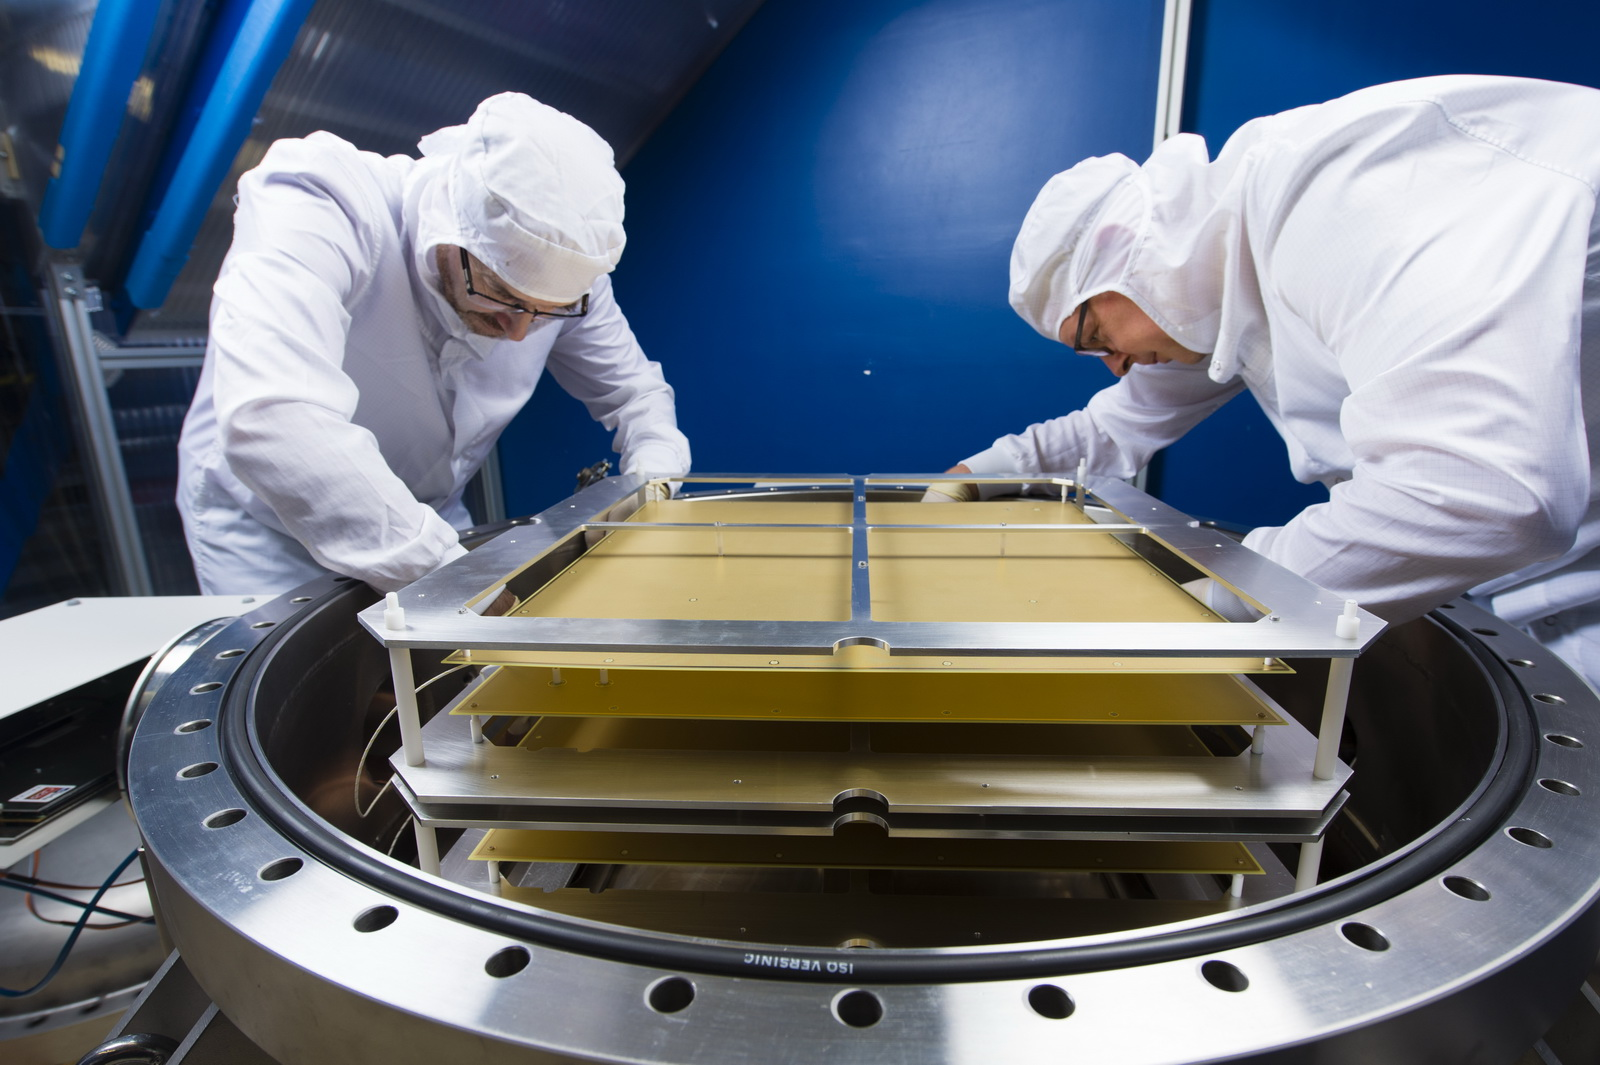
\includegraphics[width=\textwidth,keepaspectratio]{6lems_gamelle.jpg}
          \caption{\label{fig::6lems_gamelle}Enceinte haute pression avec neuf \glspl{lem} en train d'être préparés pour un test de tenue en tension.}
        \end{subfigure}
        \hfill
        \begin{subfigure}[t]{0.48\textwidth}
          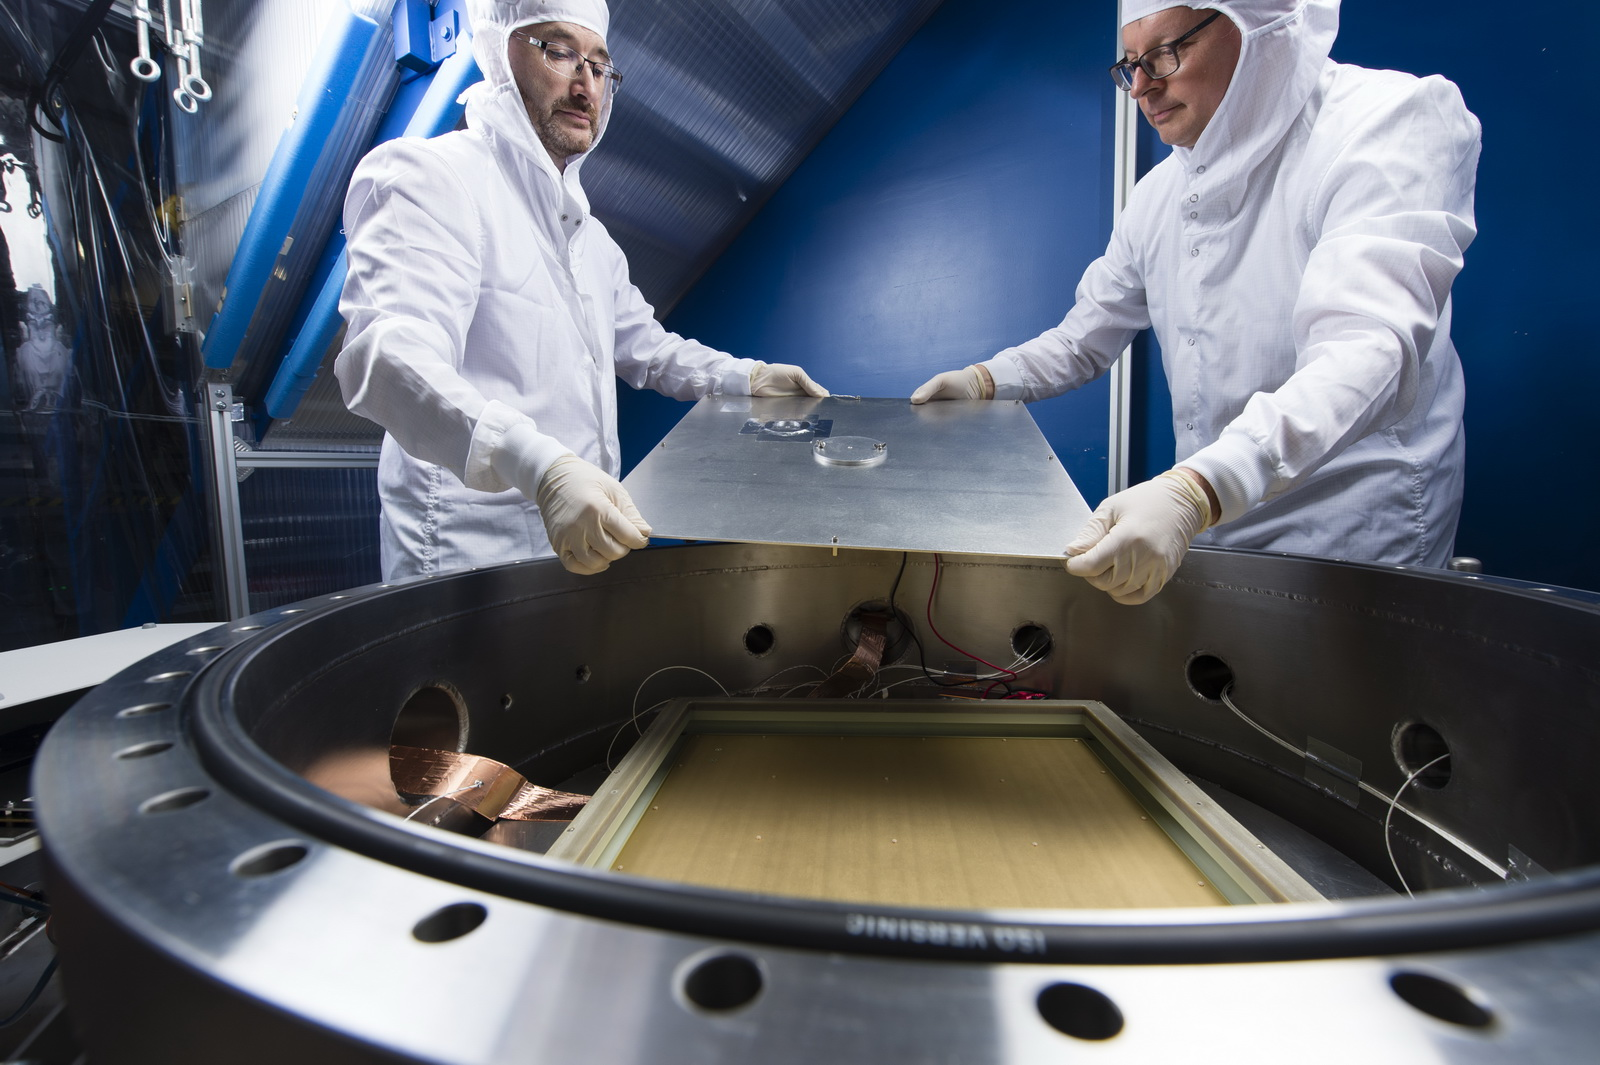
\includegraphics[width=\textwidth,keepaspectratio]{gamelle_source.jpg}
          \caption{\label{fig::gamelle_source}Enceinte haute pression avec une source d'américium, un \gls{lem} et une anode en train d'être préparés pour une mesure de gain.}
        \end{subfigure}
        \caption[Enceinte haute pression]{\label{fig::gamelle}Enceinte haute pression utilisée à Saclay pour les tests de tenue en tension et les mesures de gain des \glspl{lem} destinés au démonstrateur \SSS{}.}
      \end{figure}

      \begin{figure}[htpb]
        \begin{subfigure}[t]{0.48\textwidth}
          \centering
          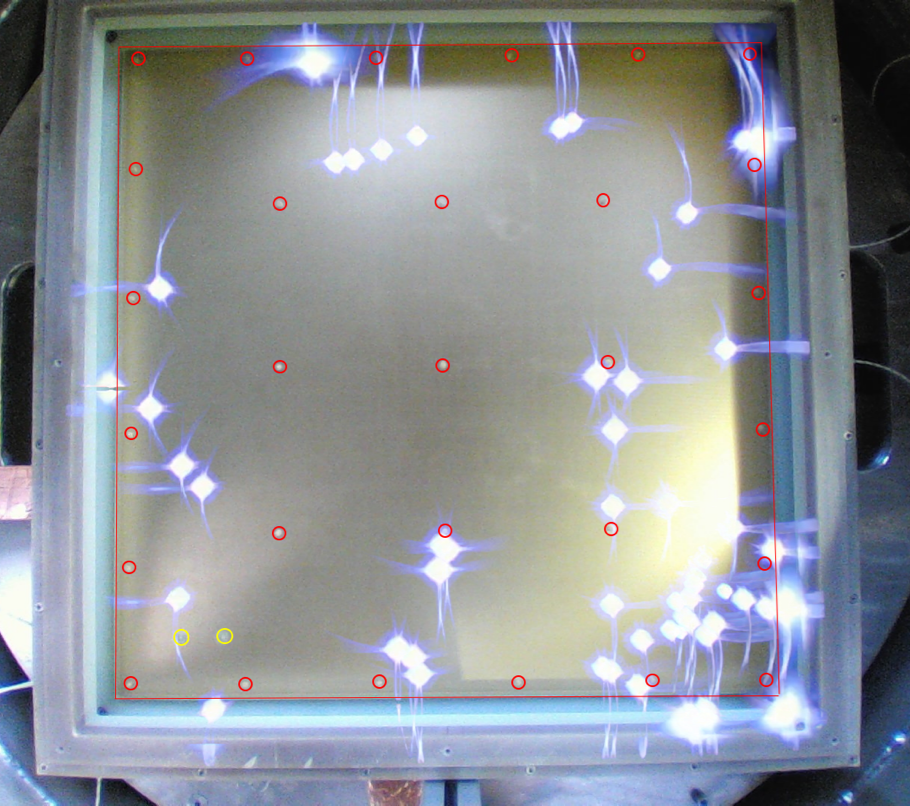
\includegraphics[width=0.8\textwidth,keepaspectratio]{sparks_34.png}
          \caption{\label{fig::sparks_34}Visualisation des décharges sur un \gls{lem} du modèle CFR-34 entre \SI{3.3}{\kilo\volt} et \SI{3.5}{\kilo\volt}. Le taux de décharge est d'environ \SI{20}{\per\hour}.}
        \end{subfigure}
        \hfill
        \begin{subfigure}[t]{0.48\textwidth}
          \centering
          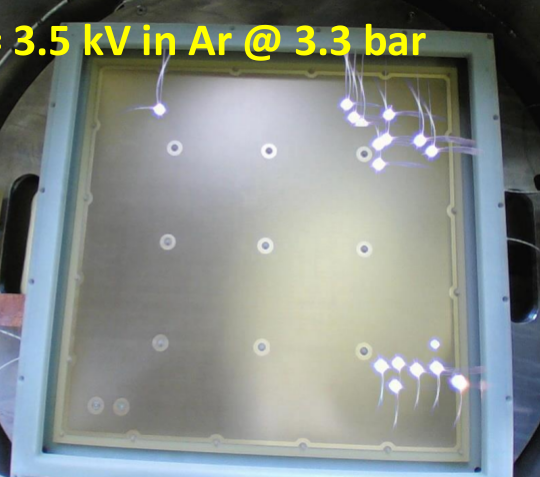
\includegraphics[width=0.8\textwidth,keepaspectratio]{sparks_35.png}
          \caption{\label{fig::sparks_35}Visualisation des décharges sur un \gls{lem} du modèle CFR-35 à \SI{3.5}{\kilo\volt}. Le taux de décharge est d'environ \SI{3}{\per\hour}.}
        \end{subfigure}
        \caption[Visualisation des décharges sur les deux modèles de LEM]{\label{fig::sparks}Visualisation des décharges sur les deux modèles de \gls{lem}.}
      \end{figure}

      Une enceinte haute pression a été construite afin d'y recréer la densité de l'argon gazeux des \glspl{dlartpc} de \gls{wa105}. Tous les \glspl{lem} du démonstrateur \SSS{} y ont été soumis à de hautes tensions afin de déterminer leur tension de claquage, et ce dans de l'air sec ainsi que dans l'argon. A également été mesuré le gain de quelques \glspl{lem} du \SSS{} grâce à une source d'américium placée dans l'enceinte.
            
      Pour les tests haute tension, neuf \glspl{lem} pouvaient être testés en même temps dans l'enceinte. La \autoref{fig::6lems_gamelle} montre  ce dispositif. Pour les mesures de gains, un seul \gls{lem} était placé, ainsi qu'une anode de lecture et la source. L'espacement entre l'anode et le \gls{lem} est le même que sur le \gls{crp}, $\SI{2}{\milli\meter}$. La cathode avec la source est située $\SI{5}{\centi\meter}$ au dessus du \gls{lem}. La \autoref{fig::gamelle_source} montre ce dispositif. Ces tests ont permis de mettre en évidence une limitation des \glspl{lem} du modèle CFR-34, utilisé dans le prototype de \TOO{}. Ces derniers présentaient un taux de claquage bien trop grand (autour de 20 par heure) au delà de \SI{3.3}{\kilo\volt}. La tension voulue étant de \SI{3.1}{\kilo\volt}, cela laissait trop peu de marge d'erreur. Comme les décharges semblaient avoir lieu essentiellement sur les bords (voir \autoref{fig::sparks}), un modèle avec des zones mortes plus grandes a été mis au point, le CFR-35, décrit en \autoref{sec::LEM}. Ce modèle présente alors un taux de claquage autour de 3 par heure à \SI{3.5}{\kilo\volt} et a été retenu pour le \SSS{}. Une étude visant à déterminer la dimension optimale des bords afin de limiter les claquages tout en conservant une zone active raisonnable est en cours avec le logiciel COMSOL Multiphysics.

    \subsection{Mesures de gain dans une enceinte haute pression}\label{sec::test_gain}

      \begin{figure}[htpb]
        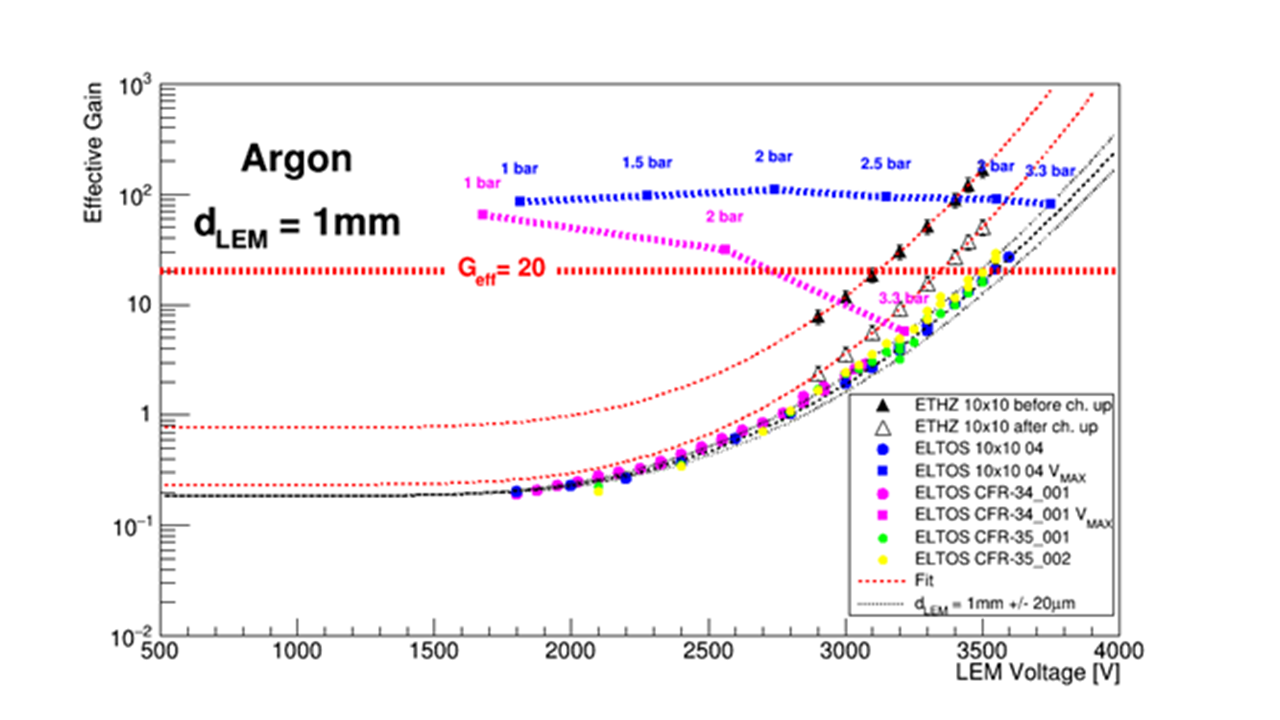
\includegraphics[width=\textwidth,keepaspectratio]{gain_2.png}
        \caption[Mesure du gain dans l'enceinte haute pression]{\label{fig::gain_gamelle}Mesure du gain dans l'enceinte haute pression pour plusieurs modèles de \glspl{lem} (ronds et carrés). Les triangles pleins sont les mesures avant charging up faites par le prototype de \threeL{}\cite{Cantini2014}, les triangles vides sont les gains attendus du \threeL{} après charging up (voir texte).}
      \end{figure}

      Des mesures de gain ont été faites dans l'enceinte haute pression pour plusieurs \glspl{lem} : des prototypes de $10\times\SI{10}{\centi\meter}$, semblables à ceux utilisés dans le prototype de \threeL{}, ainsi que des \glspl{lem} de $50\times\SI{50}{\centi\meter}$ CFR-34 et CFR-35. Plusieurs pressions ont été utilisées, allant de 1 à \SI{3.3}{\bar}, équivalent à la densité de l'argon gazeux des \glspl{dlartpc} de \gls{wa105}. Toutes ces mesures sont faites après charging up complet du \gls{lem}.

      La \autoref{fig::gain_gamelle} montre le résultat de ces mesures. Tous les \glspl{lem} testés dans l'enceinte ont un comportement identiques. Sur cette même figure sont également représentées les données du prototype de \threeL{} issues de \cite{Cantini2014} avant charging up. Un facteur de \numprint{2.7} a été utilisé pour estimer le gain après charging up de ces mêmes données, correspondant au ratio avant/après charging up mesuré dans le \threeL{} à \SI{3.4}{\kilo\volt}. On peut constater que les mesures réalisées dans l'enceinte haute pression sont inférieure au gain attendu après charging up d'après le \threeL{}. Cette différence n'est pas encore bien comprises, et une calibration précise du gain va être réalisée en effectuant des mesures avec et sans \gls{lem}. 

      Sur la même figure sont également représentés les gains maximums attendus dans l'enceinte à différentes pressions. Ces valeurs sont obtenue en mesurant la tension maximale supportée par les \glspl{lem} à ces pressions. Le gain maximum est ensuite estimé à partir de l'ajustement de l'équation \eqref{eq::gain_eff} aux gains mesurés à ces même pressions à des tensions plus basses. On constate que les \glspl{lem} de $50\times\SI{50}{\centi\meter}$  CFR-34 atteignent des tensions plus faibles que ceux de $10\times\SI{10}{\centi\meter}$.
        
    \subsection{Test de continuité des canaux de lecture des anodes}\label{sec::test_anode}

      \begin{figure}
        \begin{subfigure}[t]{0.48\textwidth}
          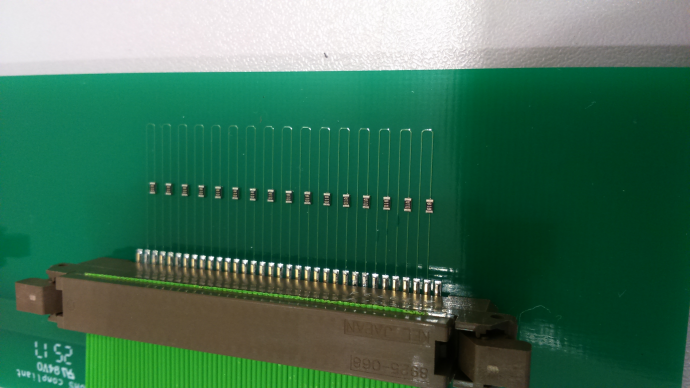
\includegraphics[width=\textwidth,keepaspectratio]{anode_card_zoom.png}
          \caption{\label{fig::anode_card_zoom}Agrandissement d'une carte de mesure. On y voit les résistances de \SI{100}{\ohm} placées entre les canaux de l'anode.}
        \end{subfigure}
        \hfill
        \begin{subfigure}[t]{0.48\textwidth}
          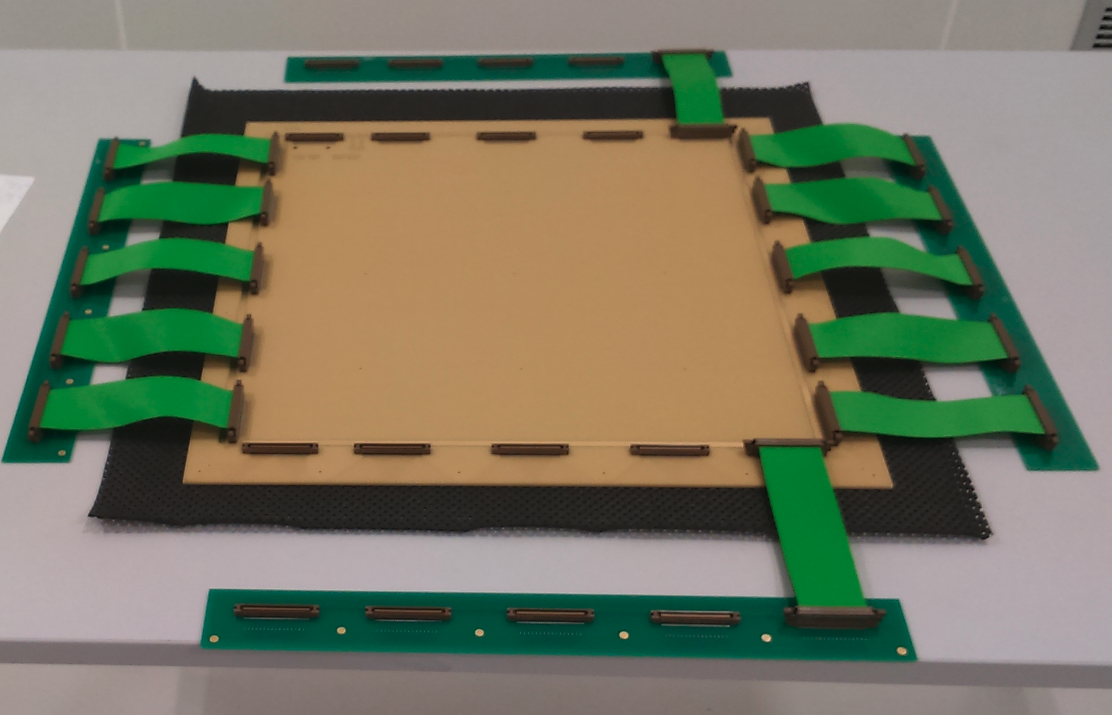
\includegraphics[width=\textwidth,keepaspectratio]{anode_carde.png}
          \caption{\label{fig::anode_card}Photo du dispositif de mesure. Les cartes de chaque côtés permettent aux \numprint{160} canaux de l'anode de n'en former plus qu'un, si aucun n'est cassé. Les cartes au dessus et en dessous servent à vérifier qu'il n'y a pas de court circuit entre les deux vues de l'anode.}
        \end{subfigure}
        \caption[Dispositif de mesure de la continuité des canaux de lecture des anodes]{\label{fig::test_anode}Dispositif de mesure de la continuité des canaux des lecture des anodes.}
      \end{figure}
      La continuité des canaux de lecture des anodes ainsi que leur isolation les uns par rapport aux autres ont été testées grâce à des \glspl{pcb} créés à cet effet. Deux jeux de deux cartes de test ont été produits et ont permis de valider les 72 anodes du démonstrateur \SSS{} et les 6 anodes de rechange.
      
      Ces cartes sont munies des mêmes connecteurs que les anodes. Elles sont faites de manière à ce qu'en branchant une carte de chaque côté de l'anode, les 160 canaux d'une vue de l'anode forment un circuit continue. Des zones de cuivres sont prévus entre chaque groupe de 32 canaux afin d'y mesurer la résistance du groupe. La \autoref{fig::test_anode} montre le dispositif de mesure.

      Entre chaque canal est insérée une résistance de $\SI{100}{\ohm}$. Ainsi, une résistance de l'ordre de $\SI{3200}{\ohm}$ est attendue pour un groupe de 32 canaux. Une résistance significativement plus faible indiquera alors que deux canaux ou plus communiquent entre eux. Une résistance infinie indique un canal coupé. En plaçant un jeux de carte sur chaque vue, il est possible de vérifier que les deux vues ne communiquent pas entre elles. Dans les trois cas il s'agit alors de mesurer la résistance entre chaque canal du groupe posant problème afin d'identifier sur quel canal se situe le problème exactement, puis d'inspecter à l'oeil les canaux de lecture incriminés. La \autoref{fig::anode_test_probleme} montre un exemple de tels canaux.

      Au final, sur toutes les anodes ainsi testées, 10 ont posé problème. Parmi ces 10 anodes, 6 avaient des problèmes sur des canaux au bord de l'anode, où l'on ne s'attend pas à collecter de charge à cause des zones mortes des \glspl{lem} (voir \autoref{sec::dead_zones}) et ont donc été gardées. Les quatre autres ont été remplacées.

      \begin{figure}
%        \begin{minipage}{0.4\textwidth}
%          \begin{subfigure}{0.1\textwidth}
%            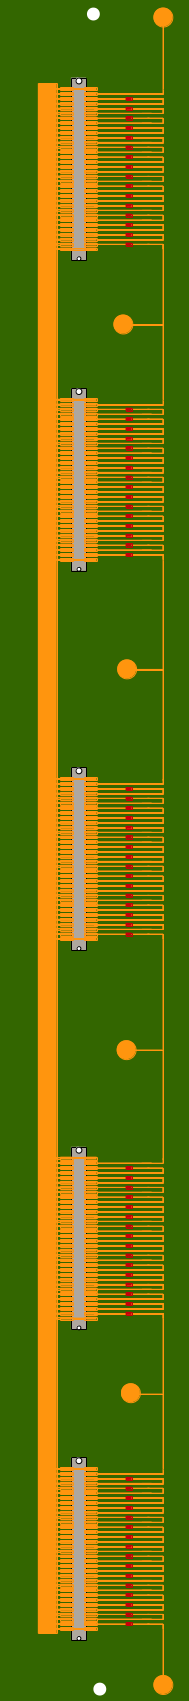
\includegraphics[width=\textwidth, keepaspectratio]{Anode_Card_left.png}
%          \end{subfigure}
%          \hfill
%          \begin{subfigure}{0.1\textwidth}
%            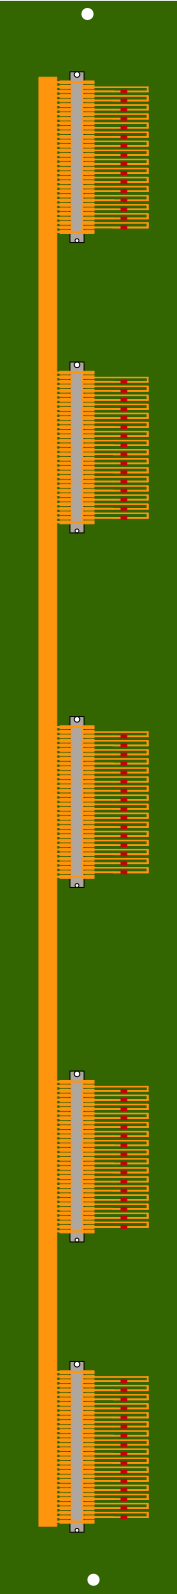
\includegraphics[width=\textwidth, keepaspectratio]{Anode_Card_right.png}
%          \end{subfigure}
%          \caption{\label{fig::anode_card_both}Schéma d'un jeu de cartes de mesure utilisé pour les tests de continuité des anodes.}
%        \end{minipage}
%        \hfill
%        \begin{minipage}{0.4\textwidth}
%          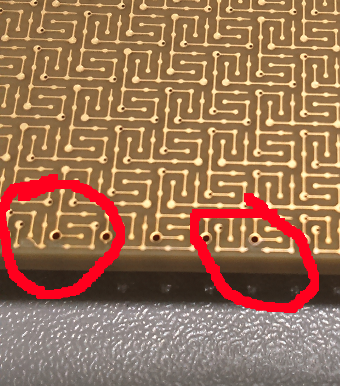
\includegraphics[width=\textwidth,keepaspectratio]{anode_problem_zoom.png}
%          \caption{\label{fig::anode_test_probleme}Photo de canaux défaillant sur le bord d'une anode.}
%        \end{minipage}
        \centering
        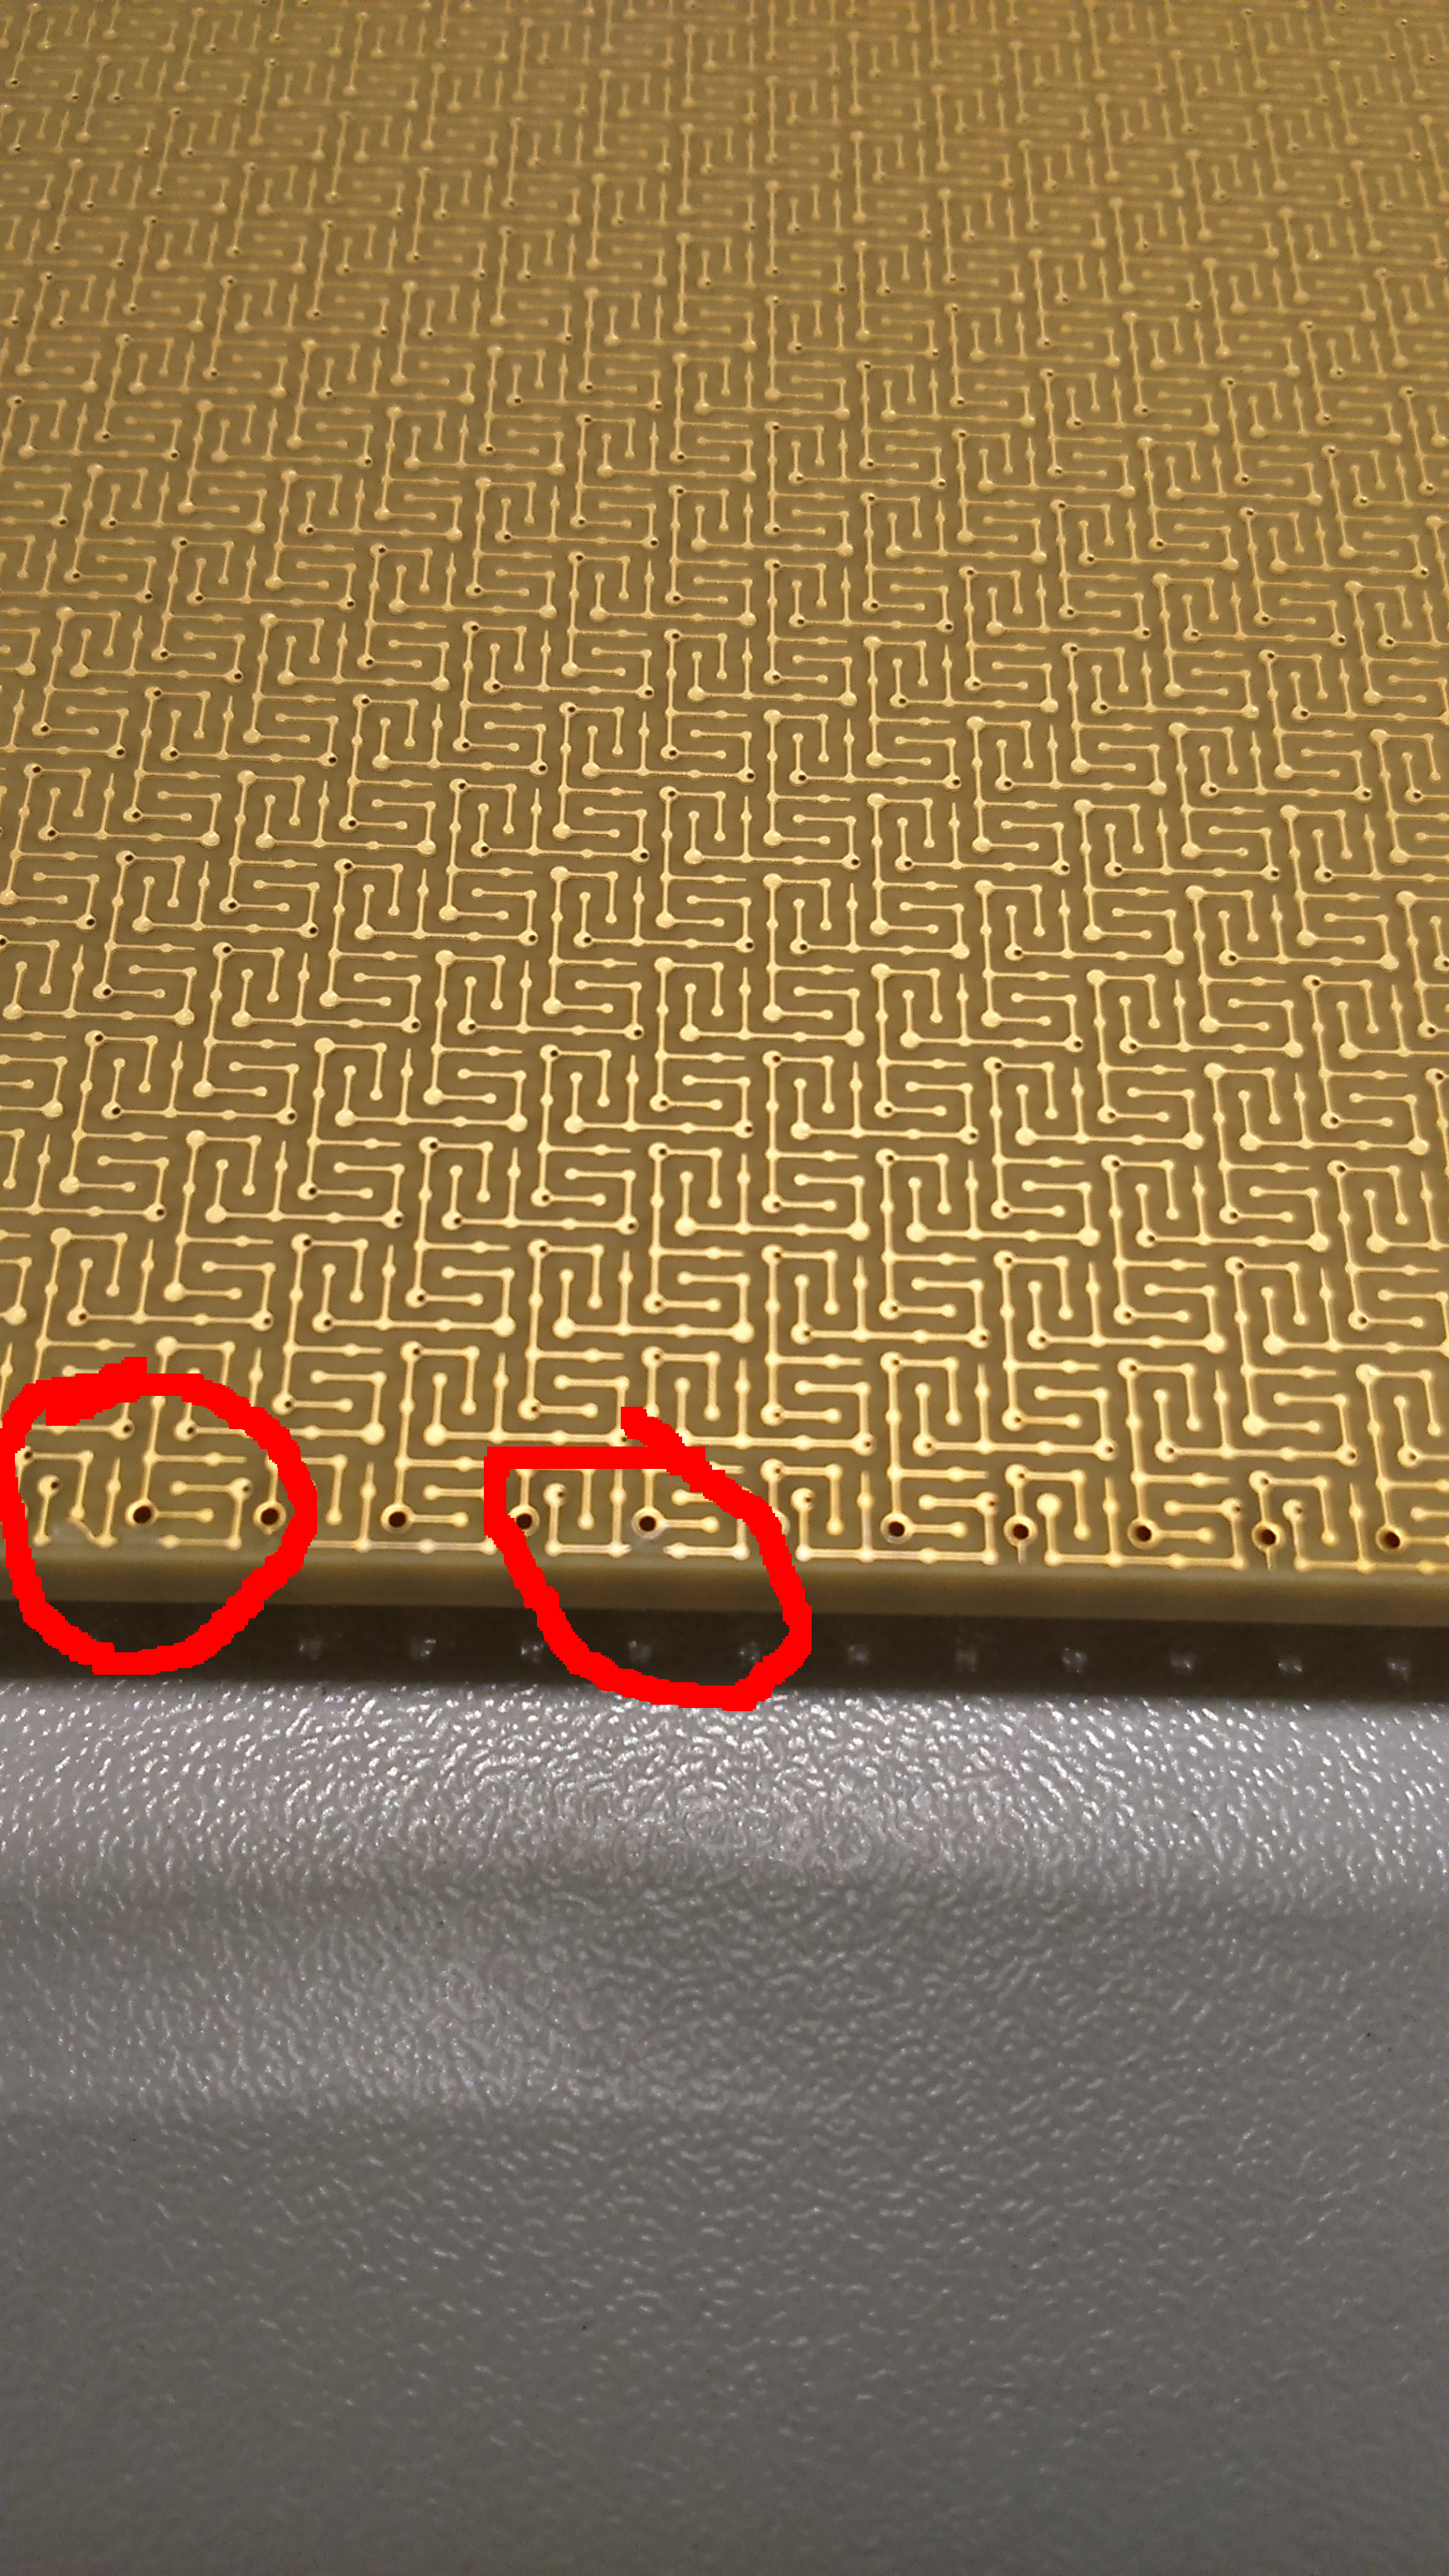
\includegraphics[width=0.6\textwidth,keepaspectratio]{anode_test_probleme.png}
        \caption[Photo de canaux défaillant sur le bord d'une anode]{\label{fig::anode_test_probleme}Photo de canaux défaillant sur le bord d'une anode.}
      \end{figure}

    \subsection{Test des CRP dans une boite cryogénique au CERN}\label{sec::cold_box}
      
      \begin{figure}
        \centering
        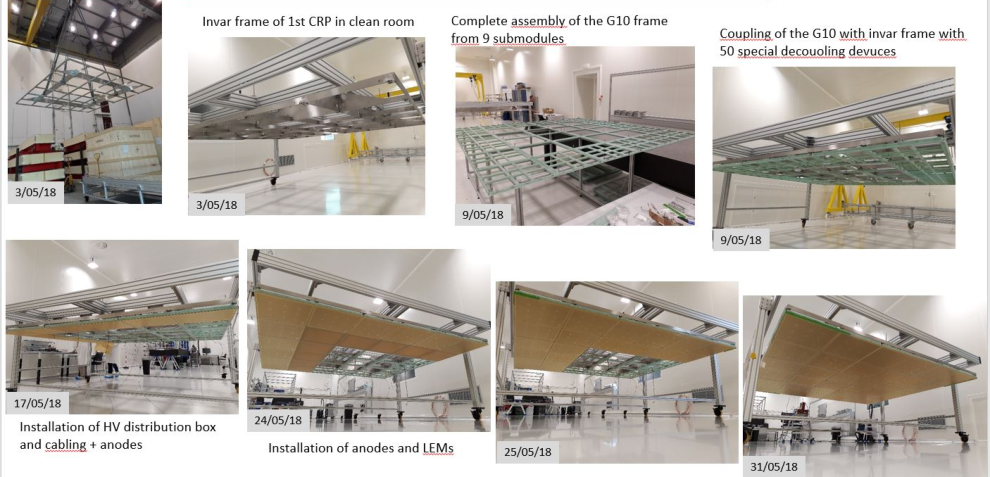
\includegraphics[width=\textwidth,keepaspectratio]{crp_assembly.pdf}
        \caption[Assemblage d'un CRP au CERN]{\label{fig::crp_assembly}Assemblage d'un \gls{crp} au \gls{cern}.}
      \end{figure}
      
      \begin{figure}
        \centering
        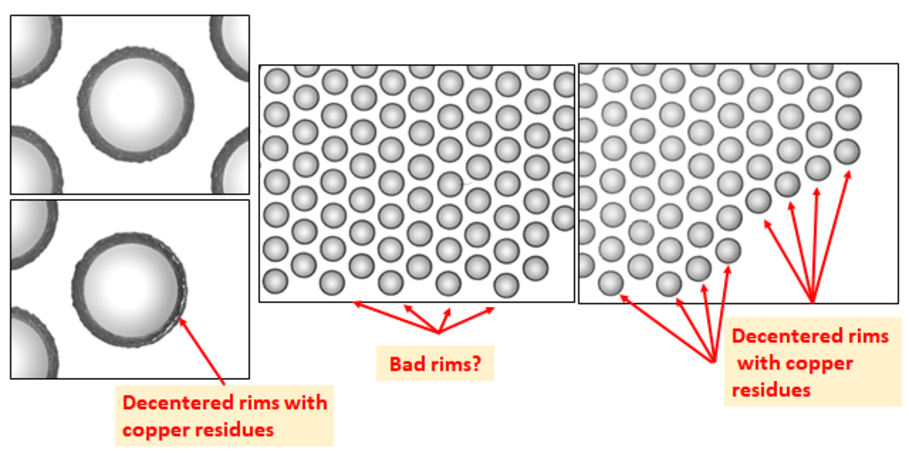
\includegraphics[width=0.8\textwidth,keepaspectratio]{copperresidues.pdf}
        \caption[Résidus de cuivre sur certains RIMs]{\label{fig::copperresidues}Résidus de cuivre sur les RIMs de trous au bord d'un \gls{lem} présentant des traces de carbonisation.}
      \end{figure}

      Après assemblage au \gls{cern} (\autoref{fig::crp_assembly}) les  \glspl{crp} du démonstrateur \SSS{} ont été testés entre Juin et Décembre 2018 dans des conditions de pression et température équivalente à celles qui seront dans le démonstrateur, grâce à une boite cryogénique construite à cet effet au \gls{cern} (voir \autoref{fig::coldbox}). Cette enceinte a testé les tenues en tension des \glspl{lem} et de la grille et peut contenir un \gls{crp} complet. Elle est équipée de capteurs permettant d'enregistrer en temps réel la pression et la température à plusieurs endroits ainsi que le niveau d'argon liquide, permettant d'estimer la planéité du \gls{crp}. 
%L'alimentation se fait comme dans le démonstrateur : les face basses des \glspl{lem} sont chacune alimentée par des canaux dédiés, les faces hautes sont groupées par 6. La grille est également alimentée par un canal dédié. 
      Un programme en python permet de suivre en direct l'évolution des différents courants et tensions des \glspl{lem} et de détecter les décharges (voir \autoref{fig::coldbox_current_voltage}). Quand plusieurs décharges arrivent sur un laps de temps relativement court (une décharge par minute environ), la tension est diminuée pour éviter d'abîmer les \glspl{lem}, le but étant de tenir plusieurs jours à une même tension, avec des décharges peu nombreuses et très espacées en temps.

      \begin{figure}[htpb]
        \centering
        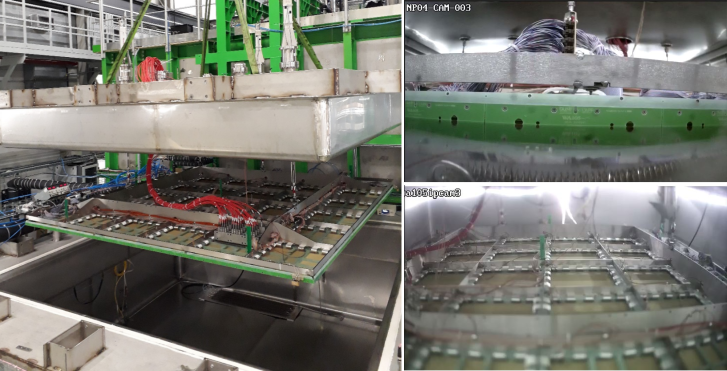
\includegraphics[width=\textwidth]{crp_in_coldbox.png}
        \caption[Un CRP dans la boîte cryogénique au CERN]{\label{fig::coldbox}Un \gls{crp} dans la boîte cryogénique au \gls{cern}.}
      \end{figure}

      La planéité des \glspl{crp}, estimée en comparant les valeurs de capteurs de niveau d'argon liquide répartis sur le pourtour de chaque \gls{crp}, est inférieur à \SI{1.75}{\milli\meter}. Cette planéité aura un impact sur le gain à travers la température dans les \glspl{lem}, qui suit un gradient dans le gaz, et à travers l'efficacité d'extraction qui dépend du champ électrique et donc de la distance grille-\gls{lem} ainsi que de la position de l'interface entre la grille et les \glspl{lem}. L'impact d'une déformation du \gls{crp} est discuté dans le \autoref{chap::5} quand nous parlerons des déformations de celui du \TOO{}. Une déformation de \SI{1.75}{\milli\meter}, à une tension d'extraction de \SI{2.5}{\kilo\volt}, aura une influence sur le gain inférieur au pourcent.

      \begin{figure}[htpb]
        \centering
        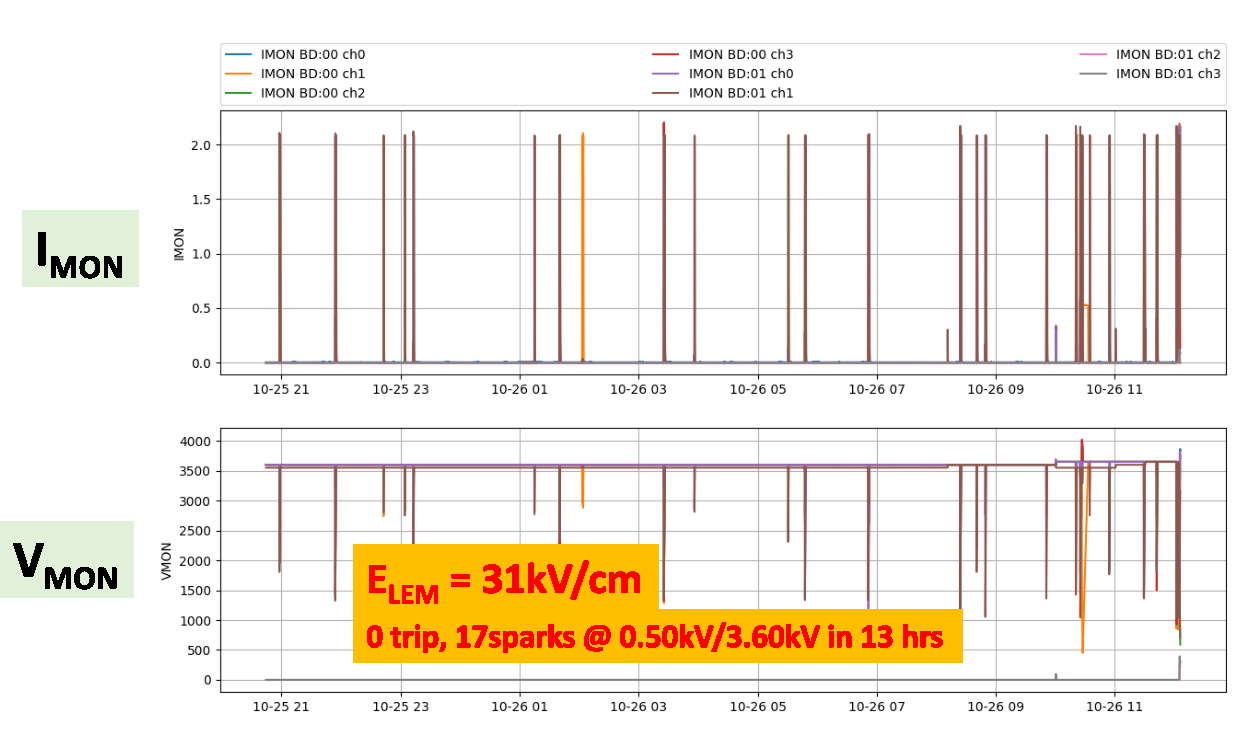
\includegraphics[width=\textwidth]{coldbox_current_voltage.pdf}
        \caption[Décharges observées dans la boîte cryogénique]{\label{fig::coldbox_current_voltage}Exemple de décharges observées dans la boîte cryogénique, pour une tension à travers le \gls{lem} de \SI{3.1}{\kilo\volt}, durant treize heures.}
      \end{figure}
    
      Les deux \glspl{crp} sont restés stables durant plusieurs semaines à la tension voulue de \SI{3.1}{\kilo\volt}, ce qui correspond à un gain attendu de 20. Le taux de décharge était de une par heure par \gls{crp}, correspondant à un temps mort d'environ \numprint{0.3}\,\%, ce qui est acceptable pour \gls{dune}. Les grilles d'extraction ont tenu la tension nominale de \SI{7.5}{\kilo\volt}. 

      Une fois sortis de la boîte, les \glspl{crp} ont été inspecté et il a été remarqué que plusieurs \glspl{lem} présentaient des traces de carbonisation dans des coins. Après nettoyage, une observation a révélé que des résidus de cuivre étaient présent sur les RIMs (\autoref{fig::copperresidues}) aux bords et dans les coins proches des zones de carbonisées. Une nouvelle technique de production des \glspl{lem} a été développée au \gls{cern}, assurant une meilleure propreté des RIMs aux bords et dans les coins des \glspl{lem}. Ces nouveaux \glspl{lem} ont été envoyés à Saclay en Mai 2019, et sont en cours de test.

%L'absence d'automatisation de la gestion de la tension a fait qu'il était impossible de surveiller en permanence la stabilité, notamment durant la nuit. Des décharges ont alors eu lieu à la chaîne, et après ouverture et inspection, il a été remarqué que plusieurs \glspl{lem} présentaient des traces de carbonisation dans des coins. Après nettoyage, une observation a révélé que les RIMs étaient légèrement décentrés dans ces régions. Ces \glspl{lem} ont été nettoyés et re-testé dans l'enceinte haute pression du \gls{cea}, ils ne présentaient et aucune diminution de performances n'a été observée; le phénomène de carbonisation n'a pas pu être reproduit au \gls{cea}. En parallèle, une nouvelle technique de production des \glspl{lem} a été développé au \gls{cern}, assurant une meilleure régularité des RIMs dans les coins. Ces \glspl{lem} ont été envoyé à Saclay en Mai, et sont en cours de mesure.
        
%      Malgré ces carbonisation des coins, les deux \glspl{crp} sont restés stables à la tension voulue de \SI{3.1}{\kilo\volt}, ce qui correspond à un gain de 20 d'après les mesures du \threeL{}. Le taux de décharge était de une par heure par \gls{crp}, correspondant à un temps mort d'environ \numprint{0.3}\,\%, ce qui est acceptable pour \gls{dune}. Les grilles d'extraction ont tenu la tension nominale de \SI{7.5}{\kilo\volt}. 

      \begin{figure}
        \centering
        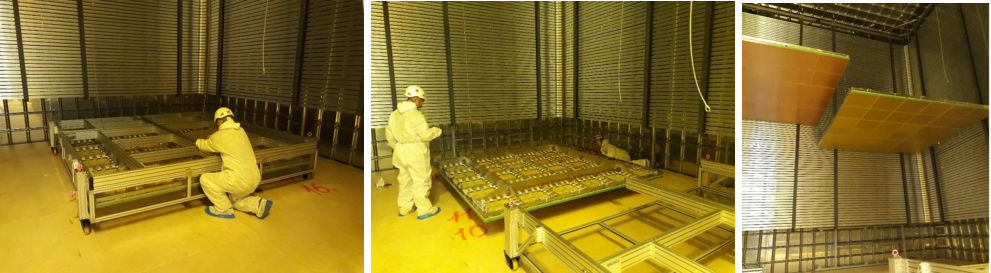
\includegraphics[width=\textwidth,keepaspectratio]{crp_installation.pdf}
        \caption[Installation de deux \gls{crp} dans le cryostat du \SSS{}]{\label{fig::crp_installation}Installation de deux \gls{crp} dans le cryostat du \SSS{}.}
      \end{figure}

      Les deux \gls{crp} non instrumentés ont également été testés en tension et en planéité, et les quatre \gls{crp} ont été installé dans le cryostat entre fin 2018 et début 2019 (\autoref{fig::crp_installation}). Dans la suite, nous nous intéressons aux champs électriques à travers le \gls{crp} et à l'impact de ces derniers sur la collection de charge. Dans un premier temps, les zones dépourvues de trous d'amplification sont étudiées, puis les efficacités de collection des électrons à travers les trous d'amplification pour plusieurs champs électriques.
        
  \section{Simulation des zones mortes des LEM}\label{sec::dead_zones}
    
    Deux modèles de \glspl{lem} sont utilisés dans \gls{wa105}, chacun présentant des aires dépourvues de trous d'amplification pouvant constituer des zones mortes. Les effets de ces zones mortes sur la charge collectée et sur la résolution de la l'énergie détectée ont été simulés pour le modèle CFR-34 (utilisé dans le prototype \TOO{}). %Une première sous-section traite de la méthode de simulation, sont ensuite présentés la carte d'efficacité ainsi créée et l'impact simulé sur la résolution en énergie. Une dernière sous-section discute des limites de cette simulation.
        
    \subsection{Méthode de simulation}
        
      \subsubsection{Carte de champ avec ANSYS}
                
        \begin{figure}[htbp]
          \begin{subfigure}[t]{0.61\textwidth}
            \centering
            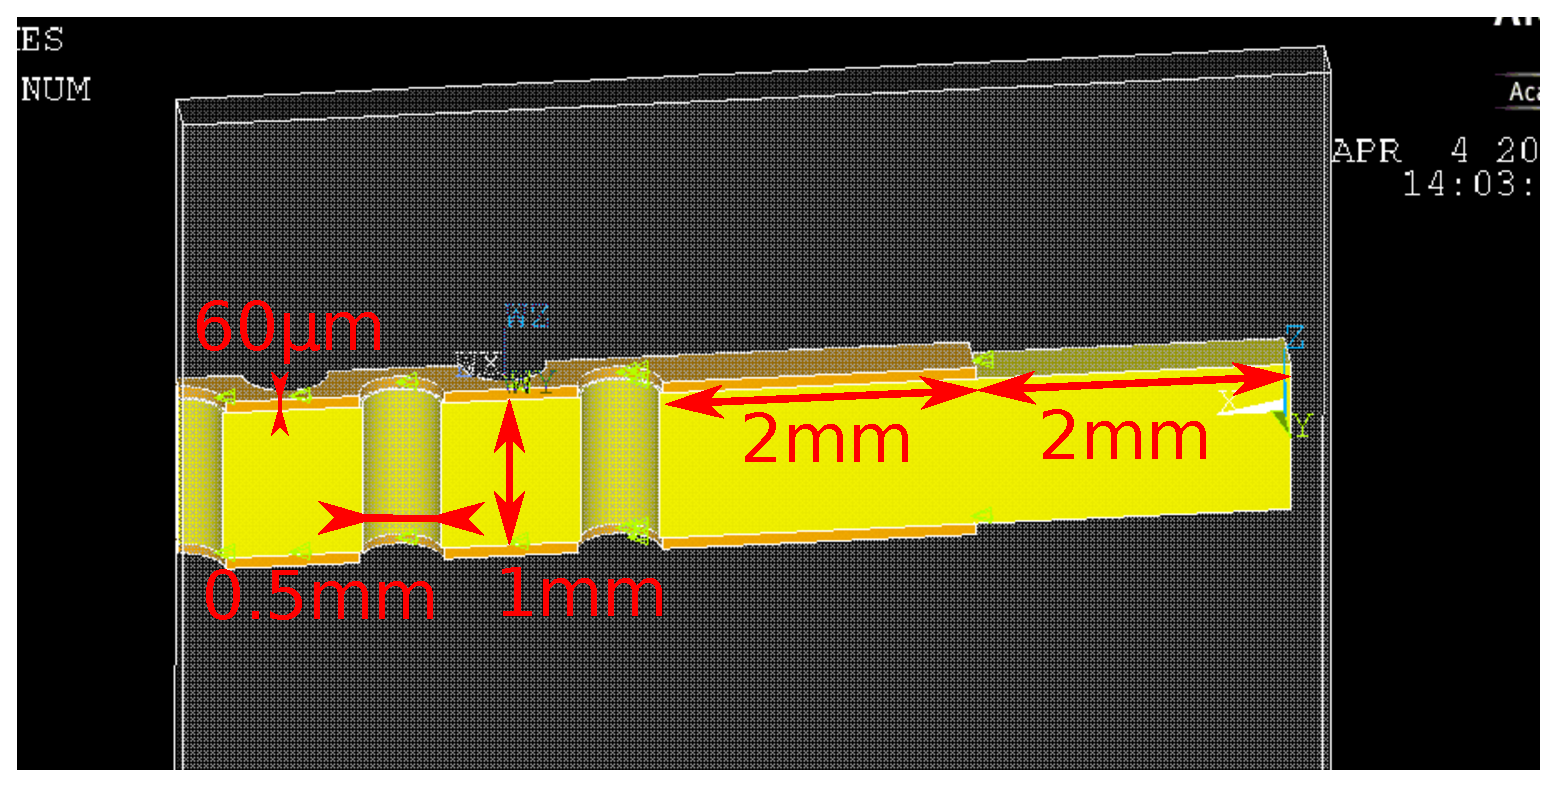
\includegraphics[width=\textwidth,keepaspectratio]{border_annotations.eps}
            \caption{\label{fig::lem_border}Bord d'un \gls{lem} modélisé avec \gls{ansys}.}
          \end{subfigure}
          \hfill
          \begin{subfigure}[t]{0.31\textwidth}
            \centering
            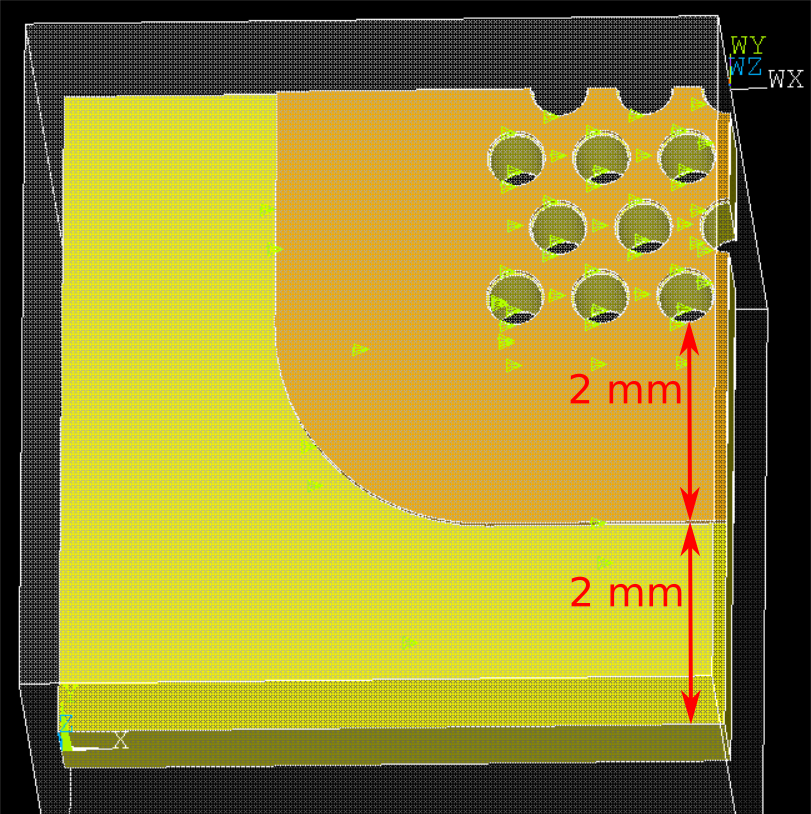
\includegraphics[width=\textwidth,keepaspectratio]{corner_annotations.png}
            \caption{\label{fig::corner}Coin d'un \gls{lem} modélisé avec \gls{ansys}.}
          \end{subfigure}\\
          \begin{subfigure}[b]{0.42\textwidth}
            \centering
            \includegraphics[width=\textwidth,keepaspectratio]{screw_annotations.png}
            \caption{\label{fig::screw}Zone autour d'un trou de vis d'un \gls{lem} modélisé avec \gls{ansys}.}
          \end{subfigure}
          \hfill
          \begin{subfigure}[b]{0.48\textwidth}
            \centering
            \includegraphics[width=\textwidth,keepaspectratio]{HT_annotations.png}
            \caption{\label{fig::HT}Zone autour d'un connecteur haute tension d'un \gls{lem} modélisé avec \gls{ansys}.}
          \end{subfigure}
          \caption[Zones mortes d'un LEM modélisé avec ANSYS]{Zones mortes d'un \gls{lem} du modèle CFR-34 utilisé dans le prototype \TOO{}, modélisées avec \gls{ansys}. Les conditions de symétrie aux limites permettent de ne simuler qu'une "maille élémentaire" de chaque géométrie.}
          \label{fig::dead_zones}
        \end{figure}
            
        Le logiciel \gls{ansys}, utilisant la méthode des éléments finis, a été utilisé pour générer la carte du champ électrique à travers le \gls{crp} pour différentes zones :
        \begin{itemize}
          \item Les bords des \glspl{lem}
          \item Les coins des \glspl{lem}
          \item Les zones autour des vis de fixation
          \item Les deux zones autour des connecteurs haute tension
        \end{itemize}
        Les bords du \gls{lem} présentent $\SI{2}{\milli\meter}$ de \gls{fr4} sans cuivre puis $\SI{2}{\milli\meter}$ de cuivre sans trous d'amplification (\autoref{fig::lem_border}), idem pour les coins (\autoref{fig::corner}). Les zones autour des vis sont simplifiées en un cercle de \gls{fr4} plein, de rayon $\SI{2.1}{\milli\meter}$ entouré d'une zone de cuivre sans trous d'amplification formant un anneau de rayon extérieur $\SI{3.2}{\milli\meter}$ (\autoref{fig::screw}). Les zones autour des connecteurs haute tension ont été modélisées de la même manière, avec un cercle de \gls{fr4} plein de $\SI{5}{\milli\meter}$ et un anneau de cuivre sans trou d'amplification de rayon extérieur $\SI{6}{\milli\meter}$ (\autoref{fig::HT}). Des conditions de symétries sont appliquées au bord des modèles afin de n'avoir à simuler que les géométries présentées en \autoref{fig::dead_zones}. 
        Les potentiels électriques utilisés pour cette simulation sont : 
        \begin{itemize}
          \item $\SI{-1000}{\volt}$ entre l'anode et le haut du \gls{lem}, correspondant à un champ d'induction de $\SI{-5}{\kilo\volt}$.
          \item $\SI{-3500}{\volt}$ à travers le \gls{lem}, correspondant à un champ d'amplification de $\SI{-35}{\kilo\volt}$.
          \item $\SI{-2500}{\volt}$ entre le bas du \gls{lem} et la grille d'extraction, correspondant à un champ d'extraction de $\SI{-2}{\kilo\volt}$ dans le liquide.
        \end{itemize}
                
      \subsubsection{Transport des charges avec GarField}
            
        \begin{figure}[htpb]
          \centering
          \includegraphics[width=0.8\textwidth,keepaspectratio]{drift_example.png}
          \caption[Dérive de 10 électrons dans la carte de champ du bord d'un LEM avec Garfield]{Dérive de 10 électrons dans un example 2D de carte de champ du bord d'un \gls{lem} créée avec \gls{ansys} par le logiciel Garfield. Le cercle rouge indique les électrons finissant leur dérive sur la zone morte, les cercles verts indiquent les électrons finissant leur dérive sur la zone d'amplification. La simulation d'avalanche n'est pas activée afin d'accélérer le calcul.}
          \label{fig::drift_example}
        \end{figure}
                
        Afin d'estimer l'impact sur la dérive des électrons des zones décrites précédemment, le logiciel GarField \cite{garfield} a été utilisé pour simuler le parcours de \numprint{10000} électrons, générés selon une distribution plate, entre la zone de transition liquide--gaz et le \gls{lem}. Les électrons n'étaient pas générés dans le liquide mais un demi-millimètre au dessus, d'une part afin de s'affranchir de l'efficacité d'extraction liquide--gaz décrite en \autoref{sec::extraction}, et d'autre part parce que GarField est incapable de simuler une dérive dans un liquide. La \autoref{fig::drift_example} montre le résultat pour une simulation de 10 électrons (l'avalanche est désactivée dans cette étude) : 5 atteignent la zone d'amplification tandis que 5 autres sont déviés sur le bords du \gls{lem}.
                
    \subsection{Résultat : carte d'efficacité}
        
      Un électron est considéré comme "bon" s'il atteint la zone d'amplification, qu'il passe ensuite à travers un trou ou non. Aucune diffusion après le \gls{lem} n'est donc prise en compte. La \autoref{fig::drift_example} montre la limite de cette zone. Pour chaque électron, la position initiale est enregistrée, ainsi que le fait qu'il ait atteint ou non la zone d'amplification. Sont alors calculées la distribution de toutes les positions initiales des électrons et la distribution des positions initiales des électrons atteignant la zone d'amplification. Le ratio de la seconds distribution sur la première défini l'efficacité de transmission en fonction de la position dans le plan $x-y$. Le résultat pour les quatre zones mortes est montré en \autoref{fig::histo_eff}.
            
      \begin{figure}[htbp]
        \begin{subfigure}[t]{0.48\textwidth}
          \centering
          \includegraphics[width=\textwidth,keepaspectratio]{histo_bar.png}
          \caption{Probabilité de transmission d'un électron en fonction de sa position initiale sous le bord d'un \gls{lem} du modèle CFR-34. La courbe pointillée correspond aux canaux de l'anode au dessus du \gls{lem}.}
        \end{subfigure}
        \hfill
        \begin{subfigure}[t]{0.48\textwidth}
          \centering
          \includegraphics[width=\textwidth,keepaspectratio]{histo_corner_screw_hv.png}
          \caption{Probabilité de transmission d'un électron en fonction de sa position initiale sous le coin, un trou de vis et un connecteur haute tension d'un \gls{lem}.}
        \end{subfigure}
        \caption[Probabilité de transmission des zones mortes d'un LEM]{\label{fig::histo_eff}Probabilité de transmission d'un électron en fonction de sa position initiale après extraction sous les différentes zone mortes d'un \gls{lem} du modèle CFR-34.}
      \end{figure}
            
      En redéfinissant la taille des bins des histogrammes ainsi obtenus à la largeur des canaux de lecture des anodes (\SI{0.3125}{\centi\meter}), il est possible de créer la carte d'efficacité complète montrée en \autoref{fig::eff_map}. Il apparaît alors que les pertes principales auront lieu sur les bords des anodes, où les premiers canaux ne devraient voir aucune charge tandis que les seconds canaux devraient voir autour de 40\,\% de la charge. Ce comportement est validé par les résultats du \TOO{} (\autoref{sec::results-311}), bien que la valeur de 40\,\% ne soit pas retrouvée.
            
%      \subsubsection{Comparaison aux données}
%            
%        A faire avec le 311.
%                %TODO à faire
            
    \subsection{Résultat : impact sur la l'énergie reconstruite}
            
      \begin{figure}[htpb]
        \begin{subfigure}{0.48\textwidth}
          \centering
          \includegraphics[width=0.9\textwidth,keepaspectratio]{eff_map.png}
          \caption{\label{fig::eff_map}Carte d'efficacité d'un \gls{lem} du modèle CFR-34. Les axes $x$ et $y$ représentent les \numprint{160} canaux des vues de l'anode se situant au dessus du \gls{lem}. La barre de couleur indique la fraction de charge qui atteindra chaque pixel ainsi formé.}
        \end{subfigure}
        \hfill
        \begin{subfigure}{0.48\textwidth}
          \centering
          \includegraphics[width=\textwidth]{electrons_new.png}
          \caption{\label{fig::electron}Simulation de l'impact de la carte d'efficacité sur la charge totale collectée d'électrons de \SI{3}{\giga\eV\per c} dans le démonstrateur \SSS{}. En noir est la charge totale collectée sans zones mortes, en prenant en compte les dispersions et les pertes dues à la recombinaison et aux impuretés dans le liquide. En rouge et la même charge mais en prenant en compte la carte d'efficacité.}
        \end{subfigure}
          \caption[Carte d'efficacité d'un LEM du modèle CFR-34 et impact sur la collection de charge]{Carte d'efficacité d'un \gls{lem} du modèle CFR-34 simulée avec \gls{ansys} et Garfield et simulation de son impact sur la collection de la charge totale d'électrons de \SI{3}{\giga\eV} avec QScan.}
      \end{figure}
        
      Cette étude a été faite avec le logiciel QScan, basé sur le framework GEANT4 pour simuler le passage de particule dans la matière. La géométrie du démonstrateur \SSS{} a été utilisée (le modèle CFR-34 était encore d'actualité au moment de la réalisation de cette étude), mais est également valable pour le prototype \TOO{}, les \glspl{crp} étant identiques mis à part les \glspl{lem}. Plusieurs types de particules à plusieurs impulsions initiales ont été générées au milieu du volume à des angles tirés aléatoirement.
            
      La charge totale arrivant à l'anode, avant reconstruction, est enregistrée avec et sans la carte d'efficacité. Les effets de diffusion longitudinale et transverse sont simulés par des répartitions gaussiennes en temps et en espace de la charge (voir \autoref{sec::ionisation}. Les \glspl{lem} sont simulés, en plus de la carte d'efficacité, par un facteur d'amplification, fixé à 1 ici. Aucune perte due à l'extraction et aucune diffusion dans le gaz n'est simulée. La \autoref{fig::electron} montre les distributions, avec et sans carte d'efficacité, de la charge totale arrivant à l'anode pour des électrons traversant le milieu d'argon liquide à une impulsion initiale de \SI{3}{\giga\eV\per c}. On peut y voir que la charge récoltée est plus basse d'environ 4\,\% avec la carte d'efficacité, comme attendu, mais également que sa distribution est plus large. La \autoref{fig::electron_mean_charge} montre les différences de la charge moyenne récoltée avec et sans carte d'efficacité pour plusieurs impulsions initiales. La \autoref{fig::electron_dispersion_charge} montre les différences de l'écart type (en pourcentage de la moyenne) de la charge récoltée avec et sans carte d'efficacité pour plusieurs impulsions initiales. L'effet sur la charge moyenne reste autour de 4\,\%, mais l'effet sur la résolution est de l'ordre de $200\%$. En comparaison (\autoref{fig::muon_mean_charge} et \autoref{fig::muon_dispersion_charge}), l'effet sur la résolution de la charge d'un muon ne dépasse pas $30\%$ (quand le muon est au minimum d'énergie), tandis que l'effet sur la moyenne est similaire à l'électron. Les zones mortes des \glspl{lem} peuvent donc avoir un effet important sur la précision de la reconstruction de l'énergie, et savoir quel facteur correctif appliquer à quel canal de lecture est nécessaire.
            
      \begin{figure}[htbp]
        \begin{subfigure}[t]{0.48\textwidth}
          \centering
          \includegraphics[width=\textwidth,keepaspectratio]{electrons_mean_charge_new.png}
          \caption{\label{fig::electron_mean_charge}Simulation de l'impact de la carte d'efficacité du CFR-34 sur la moyenne de la charge totale collectée à l'anode pour plusieurs impulsions initiales d'un électron.}
        \end{subfigure}
        \hfill
        \begin{subfigure}[t]{0.48\textwidth}
          \centering
          \includegraphics[width=\textwidth,keepaspectratio]{electrons_relative_dispersion_new.png}
          \caption{\label{fig::electron_dispersion_charge}Simulation de l'impact de la carte d'efficacité du CFR-34 sur la dispersion de la charge totale collectée à l'anode pour plusieurs impulsions initiales d'un électron.}
        \end{subfigure}
        \caption[Simulation de l'impact de la carte d'efficacité du CFR-34 sur la charge totale collectée d'électrons de plusieurs impulsions]{Simulation de l'impact de la carte d'efficacité du CFR-34 sur la charge totale collectée d'électrons de plusieurs impulsions. En noir sont les simulations sans carte d'efficacité, en rouge avec carte d'efficacité.}
      \end{figure}
            
      \begin{figure}[htbp]
        \begin{subfigure}[t]{0.48\textwidth}
          \includegraphics[width=\textwidth,keepaspectratio]{muons_mean_charge_new.png}
          \caption{\label{fig::muon_mean_charge}Simulation de l'impact de la carte d'efficacité du CFR-34 sur la moyenne de la charge totale collectée à l'anode pour plusieurs impulsions initiales d'un muon.}
        \end{subfigure}
        \hfill
        \begin{subfigure}[t]{0.48\textwidth}
          \includegraphics[width=\textwidth,keepaspectratio]{muons_relative_dispersion_new.png}
          \caption{\label{fig::muon_dispersion_charge}Simulation de l'impact de la carte d'efficacité du CFR-34 sur la dispersion de la charge totale collectée à l'anode pour plusieurs impulsions initiales d'un muon.}
        \end{subfigure}
        \caption[Simulation de l'impact de la carte d'efficacité du CFR-34 sur la charge totale collectée de muons de plusieurs impulsions]{Simulation de l'impact de la carte d'efficacité du CFR-34 sur la charge totale collectée de muons de plusieurs impulsions. En noir sont les simulations sans carte d'efficacité, en rouge avec carte d'éfficacité.}
      \end{figure}
        
    \subsection{Limites de cette simulation}
        
      Cette simulation comporte plusieurs limites.
      \begin{itemize}
        \item[$\bullet$] Elle n'a été faite que pour une configuration du champ électrique à travers le \gls{crp} fixée. Or des variations du champ d'extraction et/ou du champ d'amplification vont modifier les lignes de champs proches du \gls{lem}, il est donc possible que les probabilités de transmission en soient impactées. La méthode de simulation décrite plus haut peut tout à fait être répétée dans une étude future pour d'autre configurations du champ à travers le \gls{crp}.
        \item[$\bullet$] Cette étude n'a été faite que pour le modèle CFR-34, qui n'est pas utilisé dans le démonstrateur de \SSS{} et ne le sera pas non plus dans \gls{dune}. Les temps de calculs plus grands induits par des zones mortes plus grandes du modèle CFR-35 rendent les simulations avec \gls{ansys} beaucoup plus longues dans les coins et proche des trous de vis de de connecteur haute tension. Une simulation du bord a été réalisée, et est présentée en \autoref{fig::border_CFR_35}. L'aspect est similaire au CFR-34 : les canaux des anodes en face des zones mortes seront aveugles, le canal en marge recevra 40\,\% de la charge et les autres ne seront pas impactés.
        \item[$\bullet$] Le phénomène de charge du \gls{lem} au cours d'une opération longue d'une \gls{dlartpc} aura également un impact sur le champ électrique proche des zones mortes, où un grand nombre d'électrons va s'accumuler, déformant ainsi le champ électrique. Cet effet n'est pas pris en compte par la méthode de simulation décrite ici. Une implémentation nécessiterait de réaliser un processus itératif avec GarField et \gls{ansys}, le premier calculant le nombre d'électron s'accumulant sur le \gls{fr4}, le second recalculant une carte de champ en fonction de ces charges additionnelles.
        \item[$\bullet$] L'étude de l'impact sur la reconstruction peut être précisée en vue d'être utilisée dans le \SSS{} et \gls{dune}. D'abord en regardant la distribution non pas de l'énergie totale mais du dépôt d'énergie par unité de longueur, qui est la quantité étudiée pour la reconstruction de l'énergie déposée, et d'autre part en incluant les algorithmes de reconstruction au lieu de prendre les données de simulations vraies.
      \end{itemize}
      
      \begin{figure}[htpb]
        \centering
        \includegraphics[width=0.8\textwidth]{histo_new_bar.png}
        \caption[Probabilité de transmission d'un électron en fonction de sa position initiale sous le bord d'un LEM du modèle CFR-35]{\label{fig::border_CFR_35}Probabilité de transmission d'un électron en fonction de sa position initiale sous le bord d'un \gls{lem} du modèle CFR-35. La courbe pointillée correspond aux canaux de l'anode au dessus du \gls{lem}.}
      \end{figure}
        
  \section{Simulation des efficacités de collection de charge}\label{sec::efficacites}
    
    L'efficacité d'extraction des électrons de dérive de la phase liquide vers la phase gazeuse est décrite en \autoref{sec::extraction}, et croît avec le champ électrique dans le liquide jusqu'à atteindre 1 à \SI{3}{\kilo\volt\per\centi\meter}. Les mesures faites par le prototype de \threeL{} ont cependant montré que le gain atteint un maximum autour de \SI{2.5}{\kilo\volt\per\centi\meter} et semble même diminuer après\cite{Wu2017} (voir \autoref{fig::wu_extr}). Ceci peut peut être due à une perte d'électron au niveau de la face basse du \gls{lem} qui fait qu'une partie seulement des électrons extraits du liquide atteindront l'amplification. Cet effet, qui sera nommé \textit{efficacité de collection du \gls{lem}} dans le reste du texte, a été simulé en fonction du champ d'amplification et du champ d'extraction afin, d'une part, de vérifier cette hypothèse, et d'autre part afin d'être pris en compte dans l'estimation du gain avec le prototype de \TOO{}. Ce phénomène dépendra du champ dans le gaz et non du champ dans le liquide, aussi l'efficacité de collection du \gls{lem} est étudiée en fonction du champ dans le gaz. Dans les \glspl{lartpc} de \gls{wa105}, les champs dans le gaz et le liquide sont reliés par l'équation \eqref{eq::fields_liquid_gas}.

    Le même phénomène peut également arriver après l'amplification : tous les électrons sortant du trou peuvent ne pas arriver à l'anode, et terminer leur course sur le \gls{fr4}. Cet effet sera appelé \textit{efficacité de collection de l'anode} dans le reste du texte et a également été simulé.
    
    \subsection{Méthodes de simulation}
        
      \begin{figure}[htpb]
        \begin{subfigure}[t]{0.48\textwidth}
          \includegraphics[width=\textwidth,keepaspectratio]{ansys_geom.png}
        \end{subfigure}
        \hfill
        \begin{subfigure}[t]{0.48\textwidth}
          \includegraphics[width=\textwidth,keepaspectratio]{ansys_geom_unzoomed.png}
        \end{subfigure}
        \caption[Maille élémentaire d'un LEM modélisée avec ANSYS]{\label{fig::ansys_geom}Maille élémentaire de la disposition en nid d'abeille des trous d'amplification d'un \gls{lem} modélisée avec \gls{ansys}. Les conditions de symétrie aux bords assurent la continuité de la géométrie.}
      \end{figure}
            
      \begin{figure}[htpb]
        \begin{subfigure}[t]{0.48\textwidth}
          \includegraphics[width=\textwidth,keepaspectratio]{champ_dans_lem_extr.png}
          \caption{\label{fig::champ_dans_lem_extr}Champ électrique le long de l'axe central d'un trou d'amplification de \gls{lem} pour un champ d'amplification de \SI{32}{\kilo\volt\per\centi\meter} et plusieurs champs d'extraction dans le gaz.}
        \end{subfigure}
        \hfill
        \begin{subfigure}[t]{0.48\textwidth}
          \includegraphics[width=\textwidth,keepaspectratio]{champ_dans_lem_ind.png}
          \caption{\label{fig::champ_dans_lem_ind}Champ électrique le long de l'axe central d'un trou d'amplification de \gls{lem} pour un champ d'amplification de \SI{32}{\kilo\volt\per\centi\meter} et plusieurs champs d'induction.}
        \end{subfigure}
        \caption[Influence des variations des champs d'extraction et d'induction sur le champ électrique aux limites du LEM]{\label{fig::champ_dans_lem}Influence des variations des champs d'extraction dans le gaz et d'induction sur le champ électrique aux limites du \gls{lem}. Les zones délimitées par les rectangles jaunes et oranges représentent respectivement le \gls{fr4} et les deux épaisseurs de cuivre.}
      \end{figure}
      
      Le logiciel de simulation \gls{ansys}, utilisant la méthode des éléments finis, a été utilisé pour générer les cartes de champs de la zone entre la grille d'extraction et l'anode (voir \autoref{fig::ansys_geom}), pour plusieurs configuration de champs électriques. La supposition est faite que l'efficacité de collection du \gls{lem} n'aura aucune influence sur l'efficacité de collection de l'anode et inversement, ce qui est justifié par l'absence de variation du champ en bas du \gls{lem} quand le champ d'induction varie et inversement (voir \autoref{fig::champ_dans_lem}). En revanche, le champ d'amplification va avoir une influence sur les deux efficacités. Il a donc été décidé de simuler l'efficacité de collection du \gls{lem} (de l'anode) en fonction du champ d'amplification et du champ d'extraction (d'induction).
            
      Le logiciel GarField a été utilisé pour simuler la dérive d'électrons dans les cartes de champs produites par \gls{ansys}. Un millier d'électrons sont générés selon une distribution uniforme juste au dessus de la phase gazeuse, afin de s'affranchir de l'efficacité d'extraction \footnote{et aussi parce que GarField ne peut pas simuler des processus dans un liquide.}. Le logiciel effectue alors le transport de ces électrons dans la carte de champ (voir \cite{garfield}) ainsi que l'amplification dans les trous du \gls{lem}. Les positions de début et de fin de parcours de chaque électrons sont enregistrées. La \autoref{fig::drift_histograms} montre la distribution de ces positions. On voit que, comme supposé, des électrons peuvent finir sur la face basse du \gls{lem}, et qu'un nombre important va finir sur le \gls{fr4} à l'intérieur du trou (charging up, voir \autoref{sec::state_of_the_art}). De plus, parmi les électrons quittant la zone d'amplification, certain finiront leur course sur le RIM du haut et seront également perdus.

      \begin{figure}[htpb]
        \centering
        \includegraphics[width=0.8\textwidth]{electrons_through_lem.pdf}\\\vspace{0.1cm}
        \includegraphics[width=0.3\textwidth]{electrons_bottom_copper.pdf}
        \includegraphics[width=0.3\textwidth]{electrons_lem.pdf}
        \includegraphics[width=0.3\textwidth]{electrons_top_copper.pdf}
        \caption[Points de départ et d'arrivé des électrons à travers le LEM]{\label{fig::drift_histograms}Points de départ (haut) et d'arrivé (milieu) des électrons à travers le \gls{lem} pour un champ d'induction de \SI{5}{\kilo\volt\per\centi\meter}, un champ d'amplification de \SI{30}{\kilo\volt\per\centi\meter} un champ d'extraction dans le gaz de \SI{3}{\kilo\volt\per\centi\meter}. Les trois figures du bas sont une vue en 2D des zones où les électrons terminent leur course. Les cercles verts représentent le RIM d'un trou.}
      \end{figure}
          
      L'efficacité de collection du \gls{lem}, qui correspond à la probabilité qu'a un électron extrait du liquide d'atteindre la zone d'amplification, est définie comme le rapport entre le nombre d'électrons dépassant le RIM inférieur du \gls{lem} et le nombre d'électrons initialement générés. L'efficacité de collection de l'anode est définie comme le rapport entre, d'une part, la somme des électrons passant le RIM inférieur et des électrons générés par avalanche et, d'autre part, le nombre d'électrons arrivant à l'anode. Définit ainsi, cette efficacité correspond à un \gls{lem} avant charging up. Afin de simuler un \gls{lem} après charging up, il faudrait réaliser cette simulation de manière itérative en re-générant une carte de champ prenant en compte les électrons accumulés sur le \gls{fr4}. En effet, les lignes de champ étant modifiées par le charging up, le nombre d'électrons terminant sur les bords des trous avant le RIM supérieur devraient être moindre après charging up. Cette simulation n'a pas été faite par manque de temps.
        
      %Il y a alors deux possibilités pour définir les efficacités de collection du \gls{lem} et de l'anode. La première consiste à trouver les limites effectives de la zone d'amplification, qui est donnée par la simulation comme la région dans laquelle, à l'intérieur des \glspl{lem}, des électrons apparaissent. La probabilité de collection est alors définie comme le rapport du nombre d'électrons arrivant dans cette zone d'amplification sur le nombre d'électrons générés au départ. La probabilité de collection d'induction quant à elle est définie comme le complémentaire du rapport du nombre d'électrons qui disparaissent entre le début de la zone d'amplification et l'anode sur le nombre d'électrons qui sont entrés ou ont été créés dans la zone d'amplification. Cette définition peut correspondre à des probabilités de collection avant que le \gls{lem} ne se charge, donc en début d'exploitation d'un détecteur. Mais une fois chargé, on s'attend à ce que moins de charge disparaissent dans les trous du \gls{lem}. Cette définition, sans doute précise, est cependant difficile à mettre en œuvre pour une simulation nécessitant de simuler une centaine de configuration de champ différentes. Une méthode plus simple a été adoptée. Il s'agit, plus simplement, de définir l'efficacité de collection du \gls{lem} comme le rapport du nombre d'électrons atteignant un trou sur le nombre d'électrons générés, et l'efficacité de collection de l'anode comme le rapport du nombre d'électrons sortant du trou sur la somme du nombre d'électron créé par l'amplification et du nombre d'électron atteignant un trou. L'efficacité de collection de l'anode ainsi définie ne prend alors en compte que les électrons terminant leur course sur le RIM supérieur.            
            
    \subsection{Résultats}

      \begin{figure}[htpb]
        \begin{subfigure}{\textwidth}
          \centering
          \includegraphics[width=0.48\textwidth]{eff_lem_alone_gas.pdf}\hfill
          \includegraphics[width=0.48\textwidth]{eff_lem_alone_1D_gas.pdf}
          \caption{\label{fig::eff_lem_alone}Efficacité de collection du \gls{lem} en fonction du champ d'extraction dans le gaz et du champ d'amplification.}
        \end{subfigure}\hfill
        \begin{subfigure}{\textwidth}
          \centering
          \includegraphics[width=0.48\textwidth]{eff_anode.pdf}\hfill
          \includegraphics[width=0.48\textwidth]{eff_anode_1D.pdf}
          \caption{\label{fig::eff_anode}Efficacité de collection de l'anode en fonction du champ d'induction et du champ d'amplification.}
        \end{subfigure}
        \caption[Efficacités de collection du LEM et de l'anode en fonction des champs électriques à travers le CRP]{\label{fig::eff_coll}Efficacités de collection du \gls{lem} et de l'anode en fonction des champs électriques à travers le \gls{crp}.}
      \end{figure}

      La \autoref{fig::eff_lem_alone} montre l'efficacité de collection du \gls{lem} en fonction du champ d'amplification et du champ d'extraction dans le gaz. On constate qu'elle commence à 1 et décroît (croît) avec le champ d'extraction (d'amplification). La \autoref{fig::eff_guschin_and_combined} montre la convolution de cette efficacité à l'efficacité d'extraction décrite en \autoref{sec::extraction}, obtenue en utilisant l'équation \eqref{eq::fields_liquid_gas}. On constate qu'avec cette convolution, on retrouve bien un maximum local entre \SI{2}{\kilo\volt\per\centi\meter} et \SI{3}{\kilo\volt\per\centi\meter} dans le liquide, comme observé dans le \threeL{}. On remarque de plus que l'efficacité n'atteint jamais 1. L'efficacité de collection de l'anode, montrée sur la \autoref{fig::eff_anode}, croît avec le champ d'induction et dépend peu du champ d'amplification si ce dernier est supérieur à \SI{15}{\kilo\volt\per\centi\meter}. Cette efficacité ne sera jamais de 1 avec une induction de \SI{5}{\kilo\volt\per\centi\meter}.

      Ces simulations sont utilisées au chapitre suivant pour comparer les mesures de gain faites par le \TOO{} avec celles faites par le \threeL{}. En effet, le \TOO{} n'a pas effectué de mesures de gain à champ d'induction et d'extraction fixés, et n'a pas atteint les tensions nominales pour ces champs, aussi faut-il corriger la charge mesurées avec les efficacités simulées ici pour se ramener aux valeurs de champs du \threeL{}.

    \subsection{Mesures à Saclay avec des LEM et anodes de \texorpdfstring{$10\times\SI{10}{\cm\squared}$}{10x10cm2} }

      \begin{figure}[htpb]
        \begin{subfigure}{0.48\textwidth}
          \centering
          \includegraphics[width=\textwidth]{eff_lem_gamelle.pdf}
          \caption{\label{fig::eff_lem_gamelle}Efficacité de collection du \gls{lem} en fonction du champ d'extraction dans le gaz et du champ d'amplification. Les triangles sont les mesures faites à Saclay, normalisées à la valeur maximale de la simulation, en ronds.}
        \end{subfigure}\hfill
        \begin{subfigure}{0.48\textwidth}
          \centering
          \includegraphics[width=\textwidth]{eff_anode_gamelle.pdf}
          \caption{\label{fig::eff_anode_gamelle}Efficacité de collection de l'anode en fonction du champ d'induction et du champ d'amplification. Les triangles sont les mesures faites à Saclay à différents champs d'amplification, normalisées à la valeur maximale de la simulation à ces mêmes champs, en ronds.}
        \end{subfigure}
        \caption[Comparaison aux mesures des simulations des efficacités de collection du LEM et de l'anode en fonction des champs électriques à travers le CRP]{\label{fig::eff_gamelle}Comparaison aux mesures des simulations des comportement des efficacités de collection du LEM et de l'anode en fonction des champs électriques à travers le CRP.}
      \end{figure}
      
      L'enceinte haute pression utilisée pour tester la tenue en tension des \glspl{lem} a permit de mesurer le gain en fonction du champ d'induction et du champ d'extraction dans le gaz. Avec ce dispositif il n'est pas possible d'avoir une valeur absolue des efficacités de collections, ces dernières ne pouvant pas être décorrélées de l'amplification dans le \gls{lem}, mais il est possible de mesurer leur comportement et de les comparer aux simulations. Les mesures ont été faites pour des champs d'inductions allant de \SI{0}{\kilo\volt\per\centi\meter} à \SI{5}{\kilo\volt\per\centi\meter} avec des champs d'amplification allant de \SI{26}{\kilo\volt\per\centi\meter} à \SI{34}{\kilo\volt\per\centi\meter}, et pour des champs d'extraction allant de \SI{0.4}{\kilo\volt\per\centi\meter} à \SI{1.5}{\kilo\volt\per\centi\meter} avec un champ d'amplification de \SI{30}{\kilo\volt\per\centi\meter}. L'alimentation haute tension ne permettait pas de mettre des champs d'extraction plus haut. Ces mesures ayant été faites après des mesures de gain, le charging up était fini. 

      La \autoref{fig::eff_gamelle} montre ces mesures, à gauche pour l'efficacité de collection du \gls{lem} et à droite pour l'efficacité de collection de l'anode. Pour chaque valeur de champ d'amplification, les gains mesurés sont normalisés à la valeur maximale d'efficacité simulée. On constate que les tendances mesurées vont dans le même sens que les tendances simulées. La simulation étant faite avant charging up et les mesures après, une différence était attendue pour l'efficacité de collection de l'anode, et l'on observe bien que l'efficacité simulée croît plus vite à bas champ que l'efficacité mesurée.

      En revanche, ce charging up de devrait pas avoir d'impact sur l'efficacité de collection du \gls{lem}. En effets, les simulations prédisent que les électrons finissent sur le cuivre, et donc sont évacués dans le circuit électrique sans s'accumuler. Les comportements de cette efficacité en fonction du champ d'extraction sont différents entre simulation et mesure à moins de \SI{1}{\kilo\volt\per\centi\meter}, mais compatibles pour les trois points entre \SI{1}{\kilo\volt\per\centi\meter} et \SI{1.5}{\kilo\volt\per\centi\meter}. Les champs d'extraction dans le gaz utilisés dans le \TOO{} sont tous supérieurs ou égaux à \SI{1}{\kilo\volt\per\centi\meter}.

%  \section{Simulation du gain}\label{sec::gain_simulation}
%    \textcolor{red}{J'ai déjà quelques plots, il faut juste que je les retrouve... mais la conclusion sera que le comportement du gain en fonction du champ électrique ne correspond pas aux mesures du 3L même en prenant en compte les efficacités de collections. L'explication proposée sera donc la génération d'électrons par effet photoélectrique avec les UV produit à l'ionisation.}
       
  \section{Conclusion et perspectives}

    Les tests décris dans ce chapitre ont permis de mettre en évidence une limitation de la tenue en tension des \glspl{lem}, qui a été prise en compte pour la réalisation du modèle CFR-35 utilisé dans le \SSS{}. Des zones mortes plus grandes permettent une meilleure tenue en tension, permettant d'atteindre les gains requis pour \gls{dune}. Cependant, comme l'ont montré les simulations décrites en \autoref{sec::dead_zones}, ceci implique une perte de zone active. Certains canaux de lecture des anodes ne recevront qu'une fraction de la charge, ce qui peut être pris en compte maintenant que cette fraction a été simulée, mais d'autres seront complètement aveugle. Des vertex ou des topologies compliquées se trouvant sous ces canaux seront mal ou pas reconstruits, pouvant entraîner une pertes d'efficacité de reconstruction. Ce phénomène reste à étudier avec un logiciel adapté afin d'optimiser les algorithmes de reconstruction.

    En parallèle, une solution permettant à la fois de réduire les zones mortes tout en prévenant les décharges est envisagée. Il s'agit de recouvrir les bords des \glspl{lem} avec de l'isolant. En effet, des simulations faites avec COMSOL Multiphysics ont montré que des champs électriques très intenses (de l'ordre de la centaine de millier de volt par centimètre) peuvent se trouver à la limite du cuivre et du \gls{fr4}, sur les bords. Recouvrir ces zones d'isolant permettra de prévenir les décharges. Des tests préliminaires vont être réalisés avec des \glspl{lem} du modèle CFR-35 et du capton, une technique de production adaptée à la taille des bords du modèle CFR-34 est en cours de développement.

    La simulations faites avec \gls{ansys} et Garfield a permis de mettre en évidence le faite que l'efficacité de collection du \gls{lem} décroît avec le champ présent dans le gaz entre l'interface liquide-gaz et le \gls{lem}. Ceci se traduit par la présence d'un plateau d'efficacité une fois prise en compte l'efficacité d'extraction liquide-gaz. Ce plateau, bien qu'inférieur à 1, se situe à des tensions comprises entre \SI{2}{\kilo\volt} et \SI{3}{\kilo\volt} pour les \glspl{crp} du \SSS{}, tensions qui ont été atteintes dans la boîte cryogénique. De fait, les variations de la planéité de ces \glspl{crp}, inférieur à \SI{1.75}{\milli\meter}, auront un impact négligeable sur l'efficacité combinée d'extraction et de collection quand bien même elles modifieraient un peu les champs électriques.

    La simulation de l'efficacité de collection de l'anode en fonction du champ d'induction a été faite pour un \gls{lem} avant charging up et a été comparée au comportement du gain en fonction du champ d'induction avec un \gls{lem} après charging up, les mesures ne pouvant être faites avant dans l'enceinte haute pression du \gls{cea} Saclay. Les comportements sont similaires, aussi les résultats de cette simulation, ainsi que ceux de l'efficacité de collection du \gls{lem}, sont utilisés dans le chapitre suivant pour estimer le gain effectif dans le \TOO{} aux champs électriques utilisés dans le prototype de \threeL{}, que le \TOO{} n'a pas atteint. Une simulation d'un \gls{lem} pendant et après charging up pourra être réalisé en itérant la méthode décrite en \autoref{sec::efficacites} et en prenant en compte les modifications du champ électrique induites par l'accumulation d'électrons sur le \gls{fr4} au niveau des trous des \glspl{lem}. Une efficacité plus grande est attendue après charging up, les lignes de champs empêchant alors les électrons de finir leur course sur le \gls{fr4}.

\FloatBarrier

\printbibliography